\documentclass[12pt]{article}
%\usepackage[latin1]{inputenc}
\usepackage[utf8]{inputenc}
\usepackage{float}
\usepackage{amsmath,amsfonts}
\usepackage{graphicx}
\usepackage[authoryear]{natbib}
\usepackage[unicode=true]
 {hyperref}
%\usepackage{breakurl}

\usepackage{array}
\usepackage[centerlast,bf,justification=justified,singlelinecheck=false]{caption}
\usepackage{graphicx}
\usepackage[table]{xcolor}
\usepackage{multirow}
\usepackage{hhline}
\usepackage{calc} 
\usepackage{tabularx}
\usepackage{booktabs}  
\usepackage[flushleft]{threeparttable}
\usepackage{pdflscape}

\usepackage[title]{appendix}

\usepackage{tikz}
\usetikzlibrary{decorations.pathreplacing}

%\setlength\labelsep{0pt}

%%%%%%%%%%%%%%%%%%%%%%%%%%%%%%  PACKAGES FOR COMMENTING
% THIS ADDS TEXT BOXES IN THE MARGIN
\usepackage[colorinlistoftodos,textsize=small]{todonotes}

% IF SELECTED, COMMAND WILL NOT DISPLAY COMMENTED TEXT  
%\newcommand{\comment}[1]{}  %comment not shown

%IF SELECTED, COMMAND WILL PRINT COMMENTED TEXT IN BLUE  
\newcommand{\comment}[1]
{{\bfseries \color{red} #1}} %comment shown

\newcommand{\inputy}[1]{\input{#1}\unskip}

%%%%%%%%%%%%%%%%%%%%%%%%%%%%%% User specified LaTeX commands.

\oddsidemargin 0in \evensidemargin 0in \topmargin 0in \columnsep 10pt
\columnseprule 0pt \marginparwidth 90pt \marginparsep 11pt
\marginparpush 5pt \headheight 0pt \headsep 0pt \textheight 9in
\textwidth 6.5in

\usepackage{setspace}
\usepackage{xcolor}
\hypersetup{
    colorlinks,
    linkcolor={blue!80!black},
    citecolor={blue!80!black},
    urlcolor={blue!80!black}
}

%THIS ALLOWS US TO HIDE FACT DRAFT WAS COMPILED THE DAY OF SUBMISSION 
\usepackage{datetime2,datetime2-calc}
\DTMnewdatestyle{Myyyy}{%
  \renewcommand*{\DTMdisplaydate}[4]{\DTMmonthname{##2}~##1}%
  \renewcommand*{\DTMDisplaydate}{\DTMdisplaydate}%
}
\DTMsetdatestyle{Myyyy}

% Ryan Kellogg's custom figure note function
\DeclareTextFontCommand{\fignotefont}{\normalfont\footnotesize}
\newcommand{\fignote}[2][\linewidth]{
    \begin{minipage}[]{#1}
        \vspace{12pt}
        \fignotefont{#2}
    \end{minipage}}

\makeatletter

%COMBINE MULTIPLE TABLES IN A FLOAT	
\usepackage[position=top]{subfig}
\captionsetup{position=top}

%\@ifundefined{showcaptionsetup}{}{%
%	\PassOptionsToPackage{caption=false}{subfig}}
%\usepackage{subfig}
%\makeatother

%\renewcommand{\thesection}{\Roman{section}} 

%%%%%%%%%%%%%%%%%%%%%%%%%%%%%% END PREAMBLE %%%%%%%%%%%%%%%%%%%%%%%%%%%%%% 

\begin{document}

\title{Relinquishing Riches: \\ Auctions vs Informal Negotiations \\ in Texas Oil and Gas Leasing
\thanks{Both authors declare they have no interests, financial or otherwise, that relate to the research described in this paper, nor do they have any current ties, directly or indirectly to the energy industry. We thank participants at numerous seminars, as well as Steve Cicala, Piotr Dworczak, Aaron Flaaen, Timothy Fitzgerald, Ryan Kellogg, Peter Maniloff, and Cythina Lin Lawell for helpful comments.  Yixin Sun, Eric Karsten, Devin McNulty and Grace Park provided excellent research assistance. Code for replication available at \href{https://github.com/rlsweeney/public_cs_texas}{https://github.com/rlsweeney/public\_cs\_texas}.}
\vspace{10pt}}

\author{Thomas R. Covert \thanks{University of Chicago Booth School of Business and NBER, \protect\href{mailto:Thomas.Covert@chicagobooth.edu}{Thomas.Covert@chicagobooth.edu}.}
\\
 Richard L. Sweeney \thanks{Boston College, \protect\href{mailto:sweeneri@bc.edu}{sweeneri@bc.edu}.}}

\date{\today \\
 \vspace{0.5cm}
}
\maketitle
\begin{abstract}

This paper compares outcomes from informally negotiated oil and gas leases to those awarded via centralized auction. We focus on Texas, where legislative decisions in the early twentieth century assigned thousands of proximate parcels to different mineral allocation mechanisms. We show that during the fracking boom, which began unexpectedly decades later, auctioned leases generated at least 55 percent larger up-front payments and 40 percent more output than negotiated leases did.  These results suggest large potential gains from employing centralized, formal mechanisms in markets that traditionally allocate in an unstructured fashion, including the broader \$3 trillion market for privately owned minerals.

\bigskip{}

\noindent
JEL Codes: D44, L13, Q35

\medskip

\noindent
Keywords: Auctions, Decentralized Markets, Oil and Gas Exploration and Production

\bigskip{}
\end{abstract}
\setcounter{page}{1} \onehalfspace

\newpage

Asset owners often need to identify and choose between potential contracting partners to monetize their asset's value. For example, companies that are the target of acquisition may have multiple potential acquirers, and research institutions looking to commercialize intellectual property often decide among several interested parties. Many land transactions also look like this. How should an owner go about this process?  Decades of economic theory have characterized the relative performance of different \textit{formal} transaction mechanisms, like simultaneous bidding in auctions, bargaining following an auction, and pure sequential bargaining \citep{bulow_auctions_1996, bulow_why_2009, roberts_when_2013}.  However, in the real world, many important assets are allocated via \textit{informal}, unstructured processes, and little is known about how they perform relative to theoretical benchmarks.

In this paper, we directly measure the gains from using a centralized, theoretically high-performing mechanism, relative to using informal, decentralized transactions, in the market for mineral leases in Texas. We study a large class of lands initially set aside for public use under the Texas Constitution, on which legislative decisions made nearly one hundred years ago determined whether leases signed during the recent shale boom transacted using an auction or an informal ``negotiation.''\footnote{Throughout the paper we use the term \textit{negotiation} to refer to the informal search, bargaining and solicitation process that lessors use to award drilling rights on private land. We describe what is known about this process in Section \ref{sec:Background}.} All of the minerals within these lands belong to the state. On some of these parcels, the state allocates mineral leases using a first price auction. However, on other parcels, the Texas Relinquishment Act of 1919 grants today's private surface owners the right to negotiate terms with oil and gas companies on behalf of the state, in exchange for half of the revenues they generate.  Conversations with many parties involved in Texas leasing confirm that these negotiated leases for public minerals represent a useful analogue to the broader universe of negotiated leases for private minerals in the United States. 

Our empirical strategy compares auctioned and negotiated leases that lie in narrowly defined geographic areas, which transact at approximately the same time.  Within these location and time bins, the resource quality is the same, the information about its production potential is constant, and, as we argue in Section \ref{sec:EmpiricalStrategy}, the allocation mechanism is as good as randomly assigned.  Using detailed data from over fifteen hundred leases for publicly owned minerals in Texas between 2004 and 2016, we find that auctioned leases sell for \inputy{../output/estimates/Bonus_Grid10Yr_log.tex} log points more than similar negotiated leases do. This result is robust to a wide range of controls and sample restrictions, and is not caused by differences in the likelihood that auction and negotiation parcels have a successful transaction. The economic significance of these results is large: on average, negotiated lesses would have generated \$\inputy{../output/estimates/Bonus_Grid10Yr_log_total.tex} more up front revenue had they transacted using an auction.

In principle, this improvement in seller revenues could simply reflect a transfer from buyers to sellers. However, one theoretically appealing feature of a well designed auction is that it should allocate an asset to its highest value user. Using the same empirical strategy, we look for evidence of such allocative efficiency gains by comparing subsequent output across auctioned and negotiated leases. We find that auctioned leases produce \inputy{../output/estimates/Poisson_LeaseRevenue_Grid10Yr.tex} log points more output than negotiated leases. Combined with the fact that they also have slightly higher royalty rates, we estimate that, on average, auctions increase \textit{total} payments to sellers by about \$\inputy{../output/estimates/SellerRevenue_Grid10Yr_total.tex} per lease. 

Although we are primarily interested in the differences between auctions and negotiations, which are fundamentally transaction level mechanisms, our identifying variation, the Relinquishment Act and privatization policy changes that followed, occurs at the parcel level.  If a parcel's lease mechanism affects the likelihood of a successful transaction, then a comparison of auctions vs. negotiations must account for the missing leases that didn't happen in one mechanism but would have under the other. To address this concern, in section \ref{sec:ResultsParcels} we show that negotiation and auction \textit{parcels} are equally likely to be under lease at any point in time. We also replicate our lease regressions in the parcel cross-section, and find that auction parcels earn higher discounted payments and produce more discounted output, inclusive of parcels which never lease.

We then explore the sources of these gains. As we discuss in detail below, there are many sources of persistent differences in productivity across firms in this industry. Nevertheless, we show that while auctions allocate minerals to different firms than negotiations do, both the payment and output differences hold \textit{within} firm, suggesting that firm-lease ``match'' plays an important role in determining lease outcomes. We corroborate the importance of this channel using data on the full set of bids submitted for auctioned leases. There is a large gap between the winning and losing bids in a lease's auction, of comparable size to the average difference between bonus payments on auctioned and negotiated leases.  We also find that there are large gaps in structural estimates of bidder \textit{values} implied by these bids.  The difference between winning and losing values is correspondingly similar to the average difference between output on auctioned and negotiated leases.  Overall, the distribution of bids and implied values within an auction suggest that firm-lease match is quite important, and that our empirical strategy measures plausible differences in payment and value that a well-designed auction can deliver, relative to negotiations.  

These results contribute to a small empirical literature which compares the performance of auctions to alternative mechanisms in real world settings. \cite{roberts_when_2013} find that a sequential mechanism performs better than a simultaneous bid auction in timber sales, and \cite{gentry2018entry} find that the two mechanisms perform similarly in corporate takeovers.\footnote{There is also a corporate finance literature on mergers and acquisitions comparing auctioned and negotiated outcomes. \cite{subramanian_go-shops_2007} finds that ``Go-shop'' deals, in which private equity target firms are explicitly allowed to solicit outside bids following a negotiated acquisition offer, sell at higher prices than ``No-shop'' deals do. In contrast, \cite{boone_how_2007} find that auctioned takeover deals transact at roughly the same prices as negotiated deals do.} \cite{salz_intermediation_2017} estimates large returns from the use of intermediaries, who organize auctions on their client's behalf, in the highly decentralized market for waste collection in New York City. In each of these papers, only one mechanism is observed in the data.  To predict what would happen under a different mechanism, the authors estimate the distribution of preferences and costs using a structural model, and then compute counterfactual market outcomes under alternative mechanisms.  In contrast, we observe the results of auctions and informal negotiations on otherwise identical objects, transacting at the same time.  As a result, we can estimate the causal effects of mechanism choice on welfare relevant outcomes \emph{directly} by comparing observable outcomes of import, like seller revenue and lease output. 

A direct comparison between auctions and negotiations is useful because real-world negotiations are messy.  Conversations with industry participants suggest that informal mineral lease transactions are heterogenous, with aspects of sequential negotiation coexisting with costly landowner search effort \citep{hortacsu_product_2004,allen_search_2014,cuesta2018price}, bilateral bargaining \citep{backus_cheap_2015, backus2, larsen2021efficiency} and even take-it-or-leave-it behavior on the part of some buyers.\footnote{In Appendix \ref{app:lessor_hetero} we show that lessors with more experience and more land perform better than other negotiators. However the gap between these more sophisticated negotiators and auctions is still substantial.}  The informality and heterogeneity in this market make it unlikely that the forces driving our results would be captured by any specific formal model of negotiations. Thus, we do not interpret the evidence in this paper as validating or rejecting any existing theoretical comparisons between auctions and specific alternative mechanisms.\footnote{Indeed, our results are consistent with a variety of theoretical comparisons between simple auctions and more complicated alternatives.  We explore these interpretations in Section \ref{sec:Discussion}.}  Instead, our contribution is to demonstrate the magnitude of the gains from using a formal, implementable, theoretically attractive mechanism, in a real world setting. In that sense our paper is similar to \cite{larsen2021efficiency}. Using data from bilaterally bargained vehicle transactions, he finds that the difference in welfare between actual bargaining behavior and ``second best'' mechanisms achievable under incomplete information is much larger than the \cite{myerson1983efficient} welfare loss arising from incomplete information itself.
 
We also contribute to the large literature on the economics of oil and gas leasing in the United States.  Early work by Kenneth Hendricks and Robert Porter on the performance of auctions for mineral leases in the US Gulf of Mexico focused on the empirical relevance of common values and information asymmetries \citep{hendricks_timing_1996, hendricks_empirical_1988}. They showed that US government auctions captured approximately 100\% of the \textit{ex ante} surplus in symmetric information environments, but considerably less in asymmetric information environments. Recent work on mineral lease auctions has sought to separately identify affiliation from synergies between neighboring parcels \citep{kong_selective_2017}, measure bidder uncertainty about competition \citep{kong2016sequential}, and evaluate the choice of ``security'' sold by the winning bidder to the auctioneer \citep{bhattacharya2018bidding}. An important distinction between this paper and the existing literature is that our results speak to the performance of the \textit{private} leasing market, which constitutes approximately three quarters of all mineral rights in the United States (currently worth over \$3 trillion).  

Finally, our paper contributes to a large literature on the costs and benefits of the shale boom. There is now robust evidence of large negative externalities from fracking \citep{muehlenbachs_housing_2015,currie_hydraulic_2017}. These costs, most of which are local, must be evaluated against the (ideally local) benefits generated by the use of fracking. Previous literature on the landowner benefits of fracking were limited to analyzing partial or indirect measures of landowner revenues, due to the fact that bonus payments are not publicly recorded \citep{brown_capturing_2016,feyrer_geographic_2017,bartik_local_2017}. The unique institutional features of our setting allow us to directly observe the full set of payments received by mineral owners, including bonus payments and royalty revenue. We find that bonus payments represent two thirds of total landowner revenue earned to-date for the average lease, and by construction, they are the entirety of landowner revenues for the majority of leases that are never drilled. The fact that local payments could be made substantially larger through a more formal allocation process suggests that feasible changes to the way this market operates could meaningfully shift the local cost-benefit ratio of this technology shock.

The rest of the paper proceeds as follows. In Section \ref{sec:Background}, we describe the mineral leasing process and provide background information on our natural experiment in Texas. Section \ref{sec:Data} discusses the data we use and the filtering criteria we apply to it.  Section \ref{sec:EmpiricalStrategy} describes our empirical strategy and identification argument. Section \ref{sec:ResultsLease} describe our main results, which are at the lease level. We study the extensive margin and present parcel level results in Section \ref{sec:ResultsParcels}. In Section \ref{sec:Discussion} we discuss possible mechanisms for our results, before concluding in Section \ref{sec:Conclusion}. 

\section{Background \label{sec:Background}}
In this section, we first describe the contract structure of a mineral lease, the market institutions for leasing, and the dimensions along which some leases may end up being more or less productive (Section \ref{sec:MineralBackground}). Then, in Section \ref{sec:PSF}, we describe the history of land and mineral ownership in Texas, where a natural experiment motivates our empirical strategy.

\subsection{Mineral Exploration and Production in the United States \label{sec:MineralBackground}}
The US Energy Information Administration estimates that at the end of 2017, oil and gas companies in the United States had proved reserves of 42 billion barrels of oil and 464 trillion cubic feet of natural gas. As of December 31, 2017, these reserves were worth more than \$4.5 trillion.\footnote{According to EIA data, oil prices were \$66.73 per barrel (Brent) and natural gas prices were \$3.69 per million BTU (Henry Hub).} Although more than three quarters of these deposits lie in land owned by private individuals \citep{fitzgerald_us_2016}, landowners must partner with oil and gas exploration and production companies (E\&P) to transform their reserves into revenue. 

Partnerships between landowners and E\&P companies are formalized through mineral lease agreements, which are contracts with three key elements: a \textit{primary term} indicating how much time the lessee (the E\&P company) has to drill one or more wells; a \textit{royalty rate} providing the lessor (the landowner) with a share of any realized drilling revenues; and an up-front \textit{bonus payment} to secure the right to explore.\footnote{This contract structure has important incentive implications, as positive royalty rates provide incentives for lessees to drill later in the contract, and finite primary terms provide incentives for lessees to drill earlier in the contract.  See \citet{herrnstadt}.} Many leases also include \textit{delay rentals}, which are payments the lessee must make to the landowner in the event that drilling has not begun by the start of intermediate milestone events during the primary term. Finally, some leases have additional contractual clauses regarding operations, cleanup and other landowner protections \citep{vissing_one--many_2017}.\footnote{We study these ``lease addenda'' formally in Appendix \ref{sec:Appendix_Addenda}.} 

Lessees frequently elect not to drill any wells before the conclusion of the primary term, and even when they do, realized drilling does not always result in economically viable quantities of production. As a result, most leases never receive any royalty revenues, so bonus payments are a particularly important aspect of landowner welfare. Despite their conceptual importance in this market, little is known about the distribution of bonus payments because they are usually not recorded in the mineral leases filed in county registries. 

Mineral leases are typically initiated by E\&P companies, rather than by landowners. An E\&P company will conduct background research and decide to acquire drilling rights in a particular geographic location. During this acquisition phase, E\&P's often work through intermediaries known as ``landmen.'' One reason that E\&P companies use landmen is that a given firm's need for new mineral leases may vary over time, and the skills necessary to find landowners, verify their claim to mineral interests, and convince them to lease can be too expensive for an E\&P company to consistently maintain in-house. E\&P companies can also use landmen to sign leases on their behalf, keeping the E\&P company's identity secret from potential lessors and from competing firms.\footnote{When a landman signs a lease on behalf of an E\&P company, it must eventually ``assign'' the lease back to the company before it begins drilling.  The data we study in this setting includes all assignments, so we are usually able to determine the true identity of the E\&P company that signs a lease, even when it initially uses a landman.} 

In addition to negotiating leasing terms, the decision of \emph{which} firm to partner with is important.  During the recent shale boom, there were thousands of E\&P companies operating in Texas.  Compared to other capital intensive businesses, the oil and gas industry in America is not concentrated, with the 15 largest firms producing about half of all oil produced in Texas in 2020.  The largest firm that year, EOG Resources, represented only 7\% of total oil production.  Given the large number of firms, one might expect a fairly homogenous industry.  However, there are many reasons why a landowner might expect different E\&P companies to produce substantially more or less output, and royalties, than others.  Aside from the obvious size differences, firms differ in the technical sophistication of their engineering choices, their decisions to hire external service contractors to perform drilling and completion services, and their experience developing wells in a specific location. 

\subsection{Texas Permanent School Fund \label{sec:PSF}}

Private mineral rights are a uniquely American phenomenon. When individuals outside of the United States purchase surface rights to a piece of land, local or central governments retain ownership and authority over the minerals underground. Because Texas was originally a Spanish colony, early land transactions in Texas followed a similar pattern: when a private individual bought land, the King of Spain retained the mineral rights. 

After declaring independence in the mid $19^{\text{th}}$ century, the \textit{Republic} of Texas appropriated millions of acres of unsettled land for public use and the Texas Constitution of 1876 allocated half of this land to benefit public schools. The rules for transactions on the 8 million acres of land, largely in West Texas, contained in this ``Permanent School Fund'' (PSF), were formalized in 1895.  When PSF land was sold to private citizens, Texas, following its colonial tradition, retained the rights to exploit minerals beneath the surface. The surface owner's remedy for damages resulting from any mineral exploration and development was a payment of just \$0.10 per acre, per year. 

When oil was discovered in Texas at the turn of the $20^{\text{th}}$ century, surface owners on PSF land argued that this compensation was inadequate.\footnote{Although small quantities of oil were observed in Texas prior to that point, recovery in large quantities had proved elusive prior to the massive gusher well at Spindletop in 1901. This well is largely cited as the advent of the oil age in the United States \citep{yergin_prize_2008}.} To stave off ``armed rebellion'' by these surface owners against state lessees, the Texas legislature passed the Relinquishment Act of 1919 \citep{shields_leasing_1981}. This law, amended and reinterpreted through more than a decade of subsequent litigation, appointed the surface owner as the minerals leasing agent of the state. The arrangement continues to this day, provided that the surface owner's parcel had been acquired from the PSF by 1931.\footnote{The Texas Supreme court finalized their interpretation of the Relinquishment Act on June 29, 1931.} As a result, when an E\&P company wants to develop a Relinquishment Act (RAL) parcel, it must negotiate a lease with the surface owner, as if the surface owner owned the minerals outright.  Once the surface owner and the E\&P company reach an agreement, they submit the lease to the Texas General Land Office (GLO) for final approval. If approved, the lessee remits half of the bonus and royalty payments to the state. In exchange for acting as the state's agent, the surface owner gets to keep the other half.\footnote{This arrangement does mean that the surface owner experiences \textit{all} of the effort costs associated with negotiating a lease, but enjoys just half of the benefits of a successful lease negotiation.  In Section \ref{sec:Discussion} we explore the role that this agency issue could play in explaining this paper's results.}  Although RAL surface owners are free to decide who to transact with and what the terms of that transaction will be, they owe the state a fiduciary duty, and as such, cannot engage in any self-dealing or ``off the books'' behavior.\footnote{This is documented in the RAL Leasing Guidelines published by the GLO, available at \url{https://www.glo.texas.gov/energy-business/oil-gas/mineral-leasing/leasing/forms/Guidelines-for-Leasing-Relinquishment-Act-Lands.pdf}.  It is also specified in both the Texas Natural Resources Code and the Texas Administrative Code.  Failure to act in the state's interest can result in invalidated leases, forfeiture of the right to act as the state's agent in the future, and fines.}  

Concurrent with the settlement of the Relinquishment Act, Texas passed the Sales Act of 1931. Under this Act, subsequent land sales out of the PSF transferred nearly all mineral rights to the surface owner, under what became known as the ``Free Royalty'' system.  When an E\&P company wants to develop a Free Royalty parcel, it negotiates directly with the parcel's owner, and neither party needs to seek state approval for the lease.  While the surface owner keeps all of the bonus and royalty payments that she is able to bargain for, the firm must make an \textit{additional} royalty payment, equal to a $1/16^{\text{th}}$ share of output, to the state.  Because the state doesn't retain any bonus interest, administrative bonus data for Free Royalty leases do not exist. 

Texas continued to sell PSF land under the Free Royalty system until the 1970's, when the OPEC oil embargo and federal oil regulations prompted wide ranging changes to mineral management in Texas. Beginning in 1973, the state explicitly retained full mineral interests in all remaining PSF lands.  The state continued to sell surface rights to PSF land, but GLO manages mineral leasing in these and other unsold PSF parcels. Unlike leases on RAL parcels, or leases on the broader population of private land, the state awards leases on PSF parcels in which it has retained full mineral rights using an auction. Bidders compete for leases with a fixed primary term and royalty rate, established by GLO before the auction occurs, so the cash bids are analogous to the bonus payment on a negotiated lease. 

\section{Data \label{sec:Data}}
We obtained data from the GLO on the universe of oil and gas leases on PSF lands where the State of Texas retained full or partial mineral rights \citep{activeleases,inactiveleases}.\footnote{This data, as well as all other publicly available data used in this paper except the parcel map described in the next paragraph, is available as a part of our Data Replication Package \citep{data}.} This includes leases on RAL parcels, land that was sold by the state prior to 1931, and leases on state auction parcels, land either sold after 1973 or land that still belongs to the PSF.\footnote{Texas did not retain primary mineral ownership on Free Royalty lands sold between 1931 and 1973. As a result, GLO does not track full payment information on these parcels.} In most analyses, we focus on leases signed between 2004 and 2016, concurrent with the development of several new shale plays.  Our initial dataset includes the shape, location, size, effective date, bonus payment, primary term and royalty rate for \inputy{../output/estimates/Nsample_RAL_RAW.tex} RAL leases and \inputy{../output/estimates/Nsample_STATE_RAW.tex} State auction leases.  For all leases that eventually result in drilling, we observe monthly payments for gas and oil royalties  up through March 2019.  We combine the royalty revenue data with output price\footnote{We use the Henry Hub price for natural gas royalties and the WTI price for oil royalties \citep{oilprices, gasprices}.} information to infer monthly oil and gas production for drilled leases. Note that all administrative payment data on RAL leases, both bonuses and royalties, represents \textit{only} the state's 50\% share of total payments.  As a result, we double all RAL payments in the analyses that follow.

We spatially intersect this lease level dataset with a map of Texas Counties \citep{census} and a separate map of all parcels in the PSF \citep{p2e}.  We acquired this map from a private contractor hired by GLO to match historical records of PSF parcel information to GIS representations of those parcels.  The map identifies which mineral category each PSF parcel belongs to: Relinquishment Act, Free Royalty or minerals fully retained by Texas.  We use this map of parcels to measure differences in the likelihood of a successful lease across negotiation (RAL) and auction (non-RAL) parcels in Section \ref{sec:ExtensiveMargin}, as well as to measure parcel level outcomes in Section \ref{sec:ParcelOutcomes}. 

GLO uses first price, sealed bid auctions to allocate its non-RAL leases \citep{auctiondata}. It conducts two to four centralized auctions per year, each of which includes hundreds of parcels from the PSF and other publicly owned land funds in Texas. For every parcel that is nominated by an E\&P company, we observe a ``bid notice'' describing the parcel itself, the date that the auction will be held, and the reserve price.  Following the auction, we observe the name of each bidder who bid above the reserve, as well as their bid.  

\subsection{Sample Selection and Initial Comparisons}\label{sec:sampleSelection}
We impose a number of restrictions on these data to obtain our final sample. First, we restrict the sample to leases lying on top of a shale formation, as our empirical strategy leverages the unexpected shock to the value of land from the fracking boom which occurred decades after the Relinquishment Act.\footnote{We use the EIA's definition of shale formations in Texas, shown shaded in yellow in Figure \ref{fig:RAL_map} \citep{eiaboundaries,eiathicknessef,eiathicknesspm}.} We then exclude leases smaller than 10 acres or bigger than 1,000 acres, as parcels in the PSF are never more than 1,000 acres, and GLO rarely auctions leases that cover more than one parcel. We also remove leases where the minerals are negotiated by multiple parties, due to inheritance issues. Finally we exclude a small number of leases with missing or inconsistent information. We provide additional information on these restrictions, as well as an associated waterfall table with the number of leases surviving each cut, in Appendix \ref{sec:AppendixSampleConstruction}. The resulting dataset of \inputy{../output/estimates/Nsample_NEGOTIATION_CLEAN.tex} negotiated leases and \inputy{../output/estimates/Nsample_AUCTION_CLEAN.tex} auctioned leases is summarized in Table \ref{tab:summary_stats}. Figure \ref{fig:cohorts} demonstrates the distribution of lease types over time.  

\addtolength{\tabcolsep}{-3pt}
\begin{table}[htpb]
\begin{center}
\begin{threeparttable}
	\caption{Lease Summary Statistics by Type}
	\label{tab:summary_stats}
 	\small
	
\begin{tabular}{lrrrrrrrrrr}
\toprule
\multicolumn{1}{c}{ } & \multicolumn{4}{c}{Negotiation (N = 1061)} & \multicolumn{4}{c}{Auction (N = 454)} \\
\cmidrule(l{3pt}r{3pt}){2-5} \cmidrule(l{3pt}r{3pt}){6-9}
Variable & mean & sd & min & max & mean & sd & min & max & Difference & p-value\\
\midrule
\addlinespace[0.3em]
\multicolumn{11}{l}{\textbf{Land Characteristics}}\\
\hspace{1em}Acres & 0.29 & 0.26 & 0.01 & 0.99 & 0.36 & 0.24 & 0.01 & 0.73 & -0.07 & 0.00\\
\hspace{1em}Shape Quality & 0.94 & 0.15 & 0.08 & 1.00 & 0.96 & 0.10 & 0.24 & 1.00 & -0.02 & 0.00\\
\hspace{1em}Multiple Parcels & 0.07 & 0.25 & 0.00 & 1.00 & 0.03 & 0.16 & 0.00 & 1.00 & 0.04 & 0.00\\
\hspace{1em}Shale Thickness & 3.20 & 1.23 & 0.15 & 5.90 & 3.77 & 1.21 & 0.10 & 5.84 & -0.56 & 0.00\\
\addlinespace[0.3em]
\multicolumn{11}{l}{\textbf{Lease Characteristics}}\\
\hspace{1em}Bonus & 0.94 & 1.17 & 0.01 & 10.42 & 2.09 & 2.69 & 0.02 & 19.00 & -1.15 & 0.00\\
\hspace{1em}Term & 3.84 & 1.16 & 1.00 & 7.00 & 4.76 & 0.65 & 3.00 & 5.00 & -0.93 & 0.00\\
\hspace{1em}Royalty Rate & 0.24 & 0.02 & 0.19 & 0.25 & 0.25 & 0.01 & 0.20 & 0.25 & -0.01 & 0.00\\
\addlinespace[0.3em]
\multicolumn{11}{l}{\textbf{Lease Outcomes}}\\
\hspace{1em}Output & 1.87 & 4.76 & 0.00 & 47.07 & 2.29 & 4.98 & 0.00 & 31.71 & -0.42 & 0.13\\
\hspace{1em}Lease Production Revenue & 6.58 & 16.82 & 0.00 & 153.49 & 8.53 & 20.07 & 0.00 & 169.36 & -1.95 & 0.07\\
\hspace{1em}Total Seller Revenue & 2.69 & 4.63 & 0.02 & 45.02 & 4.56 & 5.99 & 0.03 & 44.49 & -1.86 & 0.00\\
\bottomrule
\end{tabular}

	\footnotesize
    \begin{tablenotes}
    \item \textit{Units}: acres are reported in thousands; shale thickness is reported in thousands of feet and is not available for leases overlying the parts of the Eagle Ford shale, nor for any leases overlying the Haynesville and Barnett shales (\inputy{../output/estimates/Nsample_NEGOTIATION_NOTHICK.tex} negotiation leases and \inputy{../output/estimates/Nsample_AUCTION_NOTHICK.tex} auction leases); bonus, lease revenue, and total seller revenues are all reported in thousands of nominal dollars per acre; output is reported in hundreds of barrels of oil equivalent per acre; term is reported in years.  \textit{Definitions}: shape quality is the ratio of the lease's size to the size of the convex hull containing it; we define a lease as ``drilled'' if it ever reports a royalty payment; output is the BTU-weighted discounted sum of oil and gas production observed on the lease, through March 2019, lease production revenue is the monetary value of this production at contemporaneous prices, and seller revenue is the sum of bonus payments, the mineral estate's royalty share of lease revenues, and other fees. 
    \end{tablenotes}
\end{threeparttable}
\end{center}
\end{table}

\addtolength{\tabcolsep}{3pt}

\begin{figure}
    \centering
    \caption{Sample Leases by Year and Type}
	\label{fig:cohorts}
	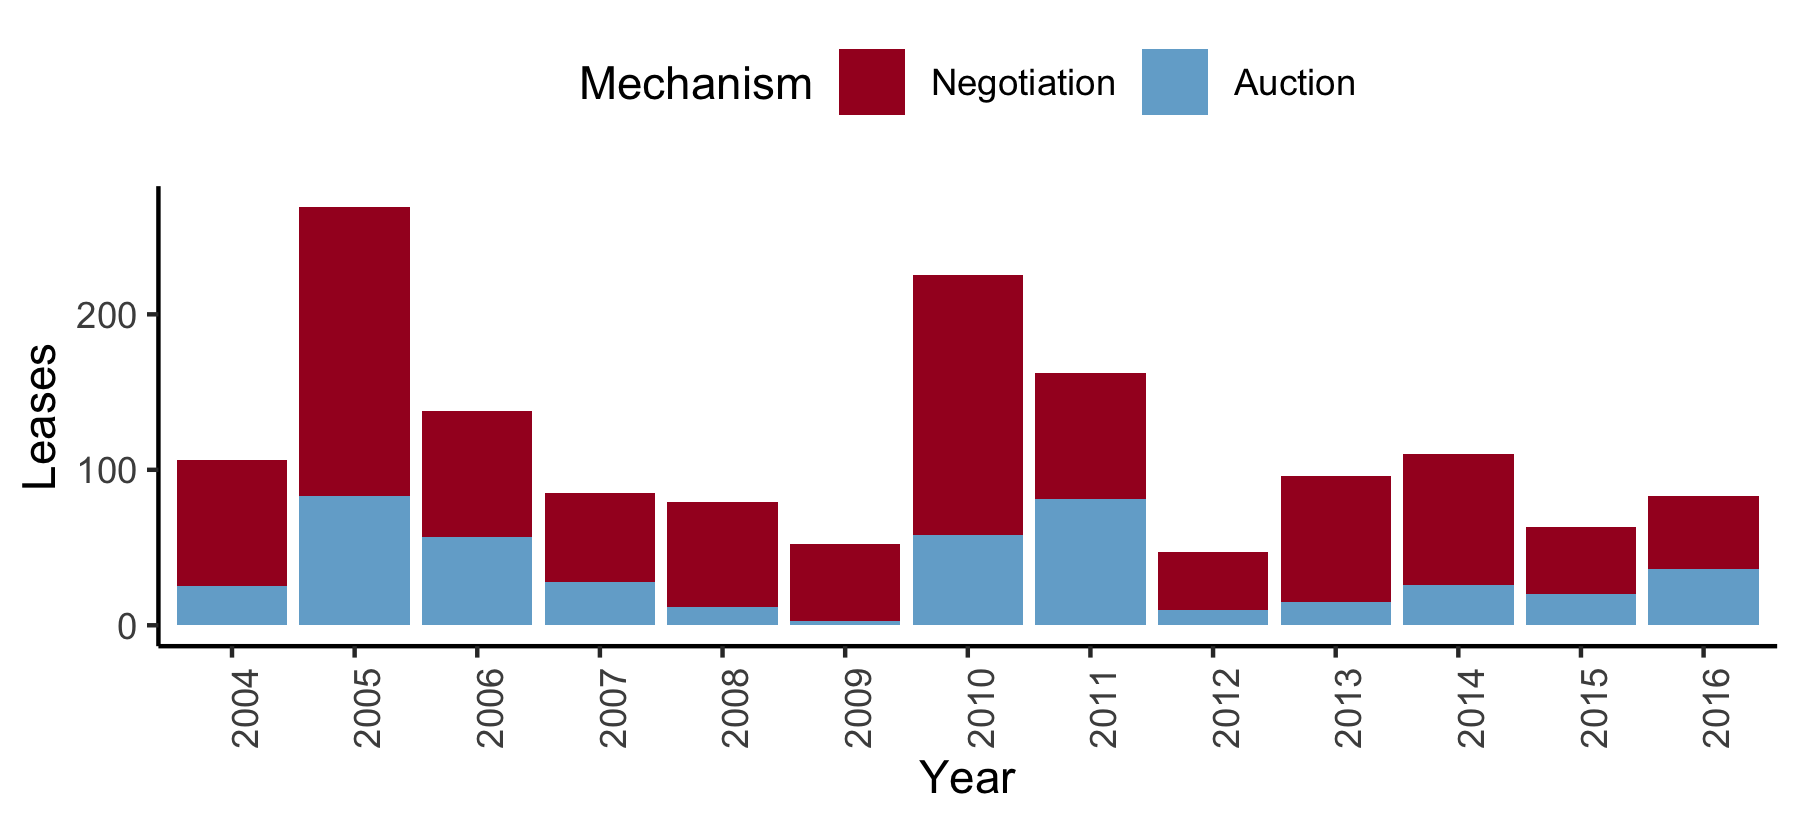
\includegraphics[width=1\textwidth]{../output/figures/cohorts.png}
\end{figure}

In the cross section, auctioned leases are larger, have slightly ``more convex'' shapes, and are less likely to cover more than one legally defined piece of land, although the differences in these measures are small. They also generate substantially higher bonus payments (per acre), pay slightly higher royalty rates, and have longer primary terms.\footnote{In principal, RAL surface owners are free to negotiate bonuses, royalty rates, and primary terms as they see fit.  However, GLO can always reject lease terms they view as insufficiently competitive, and as a result, they effectively require that negotiated royalty rates and primary terms are similar to those they are setting at auction.  Moreover, for all leases sold at the same auction, GLO sets nearly uniform royalty rates and primary term lengths.} Auctions produce more oil and gas and more associated lease revenue.  As a result, the difference in total revenues, the sum of bonus payments, royalty income on production, and other fees, is substantially larger than the difference in bonus payments alone.  Figure \ref{fig:cohorts} shows that auctions are not consistently prevalent over time, with the auction share as low as 6\% (in 2009) and as high as 50\% (in 2011).  Much of this variation is driven by differences across plays in the share of land that is governed by the Relinquishment Act and changes in which shale plays are most active over time.  Appendix Figure \ref{fig:RAL_map} shows that negotiated leases are considerably more prevalent in all shale plays except the Permian Basin in West Texas.  The variation in auction share that Figure \ref{fig:cohorts} documents is consistent with this, as the lower auction share years coincide with peak years for other shale plays, like the Eagle Ford.  These differences in timing and location underscore the importance of flexibly controlling for these factors in our empirical specifications below. 

To construct parcel level outcomes, we match all leases on PSF land to their respective parcels, using the shapefile provided by P2Energy. When leases span multiple parcels, we allocate lease outcomes to parcels proportionately based on parcel acreage.  Table \ref{tab:summary_stats_parcels} presents parcel level summary statistics. We compute the present value of lease outcomes associated with each parcel, discounting back to 2004 at a ten percent discount rate. On average, RAL ``negotiation'' parcels are more likely to have a lease, and have more leases over time, than state ``auction'' parcels.\footnote{In some circumstances, state owned minerals are negotiated, and RAL minerals are auctioned. Despite this, in this section, we describe state parcels as being ``auction'' parcels for ease of exposition, and to make the regression tables comparable to Section \ref{sec:ResultsLease}.} Negotiation parcels generate smaller total bonus payments, but have similar average realized output and production revenue. 

\addtolength{\tabcolsep}{-3pt}
\begin{table}[htpb]
\begin{center}
\begin{threeparttable}
	\caption{Parcel Summary Statistics by Type}
	\label{tab:summary_stats_parcels}
 	\small
	
\begin{tabular}{lrrrrrrrrrr}
\toprule
\multicolumn{1}{c}{ } & \multicolumn{4}{c}{Negotiation (N = 2014)} & \multicolumn{4}{c}{Auction (N = 607)} \\
\cmidrule(l{3pt}r{3pt}){2-5} \cmidrule(l{3pt}r{3pt}){6-9}
Variable & mean & sd & min & max & mean & sd & min & max & Difference & p-value\\
\midrule
\addlinespace[0.3em]
\multicolumn{11}{l}{\textbf{Land Characteristics}}\\
\hspace{1em}Acres & 0.36 & 0.27 & 0.00 & 1.29 & 0.19 & 0.23 & 0.00 & 0.92 & 0.17 & 0.00\\
\hspace{1em}Shape Quality & 0.97 & 0.10 & 0.02 & 1.00 & 0.95 & 0.12 & 0.24 & 1.00 & 0.01 & 0.01\\
\hspace{1em}Shale Thickness & 3.29 & 1.36 & 0.07 & 6.17 & 3.37 & 1.47 & 0.06 & 5.84 & -0.08 & 0.35\\
\addlinespace[0.3em]
\multicolumn{11}{l}{\textbf{Parcel Outcomes}}\\
\hspace{1em}Ever Leased & 0.72 & 0.45 & 0.00 & 1.00 & 0.55 & 0.50 & 0.00 & 1.00 & 0.17 & 0.00\\
\hspace{1em}Number of Leases & 1.72 & 2.86 & 0.00 & 61.00 & 0.84 & 0.88 & 0.00 & 4.00 & 0.88 & 0.00\\
\hspace{1em}Bonus & 0.39 & 0.57 & 0.00 & 15.77 & 0.69 & 1.23 & 0.00 & 12.71 & -0.30 & 0.00\\
\hspace{1em}Output & 1.24 & 2.97 & 0.00 & 41.82 & 1.13 & 2.67 & 0.00 & 17.28 & 0.11 & 0.38\\
\hspace{1em}Lease Production Revenue & 4.11 & 9.12 & 0.00 & 101.96 & 4.06 & 9.94 & 0.00 & 68.72 & 0.05 & 0.91\\
\hspace{1em}Total Seller Revenue & 1.46 & 2.36 & 0.00 & 26.46 & 1.80 & 3.22 & 0.00 & 26.40 & -0.34 & 0.02\\
\bottomrule
\end{tabular}

	\footnotesize
    \begin{tablenotes}
    \item \textit{Units}: acres are reported in thousands; shale thickness is reported in thousands of feet and is not available for parcels overlying the parts of the Eagle Ford shale, nor for any parcels overlying the Haynesville and Barnett shales; bonus, lease revenue, and total seller revenues are all reported in thousands of nominal dollars per acre; output is reported in hundreds of barrels of oil equivalent per acre.  \textit{Definitions}: shape quality is the ratio of the lease's size to the size of the convex hull containing it; ever leased is a dummy equal to 1 if the parcel has any active lease during 2004-2016, including leases signed before 2004; number of leases is the number of leases signed on the parcel between 2004-2013; output is the BTU-weighted discounted sum of oil and gas production observed on the parcel, through March 2019, lease production revenue is the monetary value of this production at contemporaneous prices, and seller revenue is the sum of bonus payments, the mineral estate's royalty share of lease revenues, delay rentals, and miscellaneous fees. 
    \end{tablenotes}
\end{threeparttable}
\end{center}
\end{table}
\addtolength{\tabcolsep}{3pt}

\section{Empirical Strategy \label{sec:EmpiricalStrategy}}

The single most important factor determining the value of a lease is the quality of the geological resource underneath it. Leases on parcels located above better mineral resources may transact at higher prices, attract more investment and produce more output. However, we do not observe mineral quality directly, so our empirical strategy compares auctioned and negotiated leases lying in the same narrowly defined geographic area, over which the underlying geological resource is likely to be constant. In an ideal version of these comparisons, we would have randomly assigned mechanism type, auction or informal negotiation, within narrow geographic areas among the population of private mineral owners on top of shale formations, at the eve of the fracking boom. In practice, we observe leases signed between 2004 and 2016 on PSF parcels where the state retained a mineral interest. Within this sample, a lease's mechanism type is determined not by randomization, but by the date on which the \emph{parcel} underlying it was first sold by the state. Our first identifying assumption is thus that variation in \emph{parcel privatization} dates, within a narrowly defined geographic area, is uncorrelated with the unobservable geological quality within that area.\footnote{This empirical strategy is similar to what \cite{leonard2021fragmented} employ in their study of resource development in the North Dakota Bakken Shale boom.}

Figure \ref{fig:timeline} depicts the timeline of parcel mechanism assignment. All parcels sold out of the PSF prior to 1973 transferred mineral negotiating rights to the buyer: Relinquishment Act lands until 1931, and Free Royalty lands thereafter. However, the state only retained an interest in the minerals underlying Relinquishment Act parcels. Because we observe the full payment structure on present day leases on these lands, but not for leases on parcels sold under the Free Royalty system, leases on Relinquishment Act parcels represent our ``control'' group.  By 1973, the State of Texas ended the practice of selling the rights to minerals when it sold PSF land. Leases on these subsequent land sales, as well as leases on parcels that still belong to the PSF, are awarded using a formal auction, and thus make up our ``treatment'' group.  In light of this history, our identification assumption thus requires that whether or not a parcel was sold before 1973 (so that its leases are negotiated), and, conditional on that, whether it was sold before 1931 (so that we observe leases overlying it), are both uncorrelated with unobserved geological quality, within a narrowly defined geographic area.

% the event spacing is calculated in timeline_figure_scale.xslx
\newcommand{\ticksize}{12}

\begin{figure}
    \centering
    \caption{Lease Assignment Timeline}
	\label{fig:timeline}
	
	\begin{tikzpicture}[scale=1]
	\draw [thick,->] (0,0) -- (\ticksize,0);

	\node[align=center,left] {PSF created \\ (1895)};

	\node[align=center,below] at (.15*\ticksize,0) {RAL \\ (negotiated)};
	
	\draw [thick,->] (.3*\ticksize,-1) -- (.3*\ticksize,-0.15);
	\node[align=center,below] at (.3*\ticksize,-1.15) {Relinquishment \\ Act finalized (1931)};

	\node[align=center,below,text=gray] at (.48*\ticksize,0) {Free Royalty \\ (negotiated)};
	
	\draw [thick,->] (.65*\ticksize,-1) -- (.65*\ticksize,-0.15);
	\node[align=center, below] at (.65*\ticksize,-1.15) {Free Royalty \\ sales end (1973)};

	\node[align=center] at (.325*\ticksize,0.85) {Assignment Period};
	\draw [thick,decorate,decoration={brace,amplitude=6pt,raise=0pt}] (0,0.15) -- (.65*\ticksize,0.15);

	\node[align=center,below] at (.825*\ticksize,0) {Auctions};
	
	\node[align=center, below] at (.94*\ticksize,-1.15) {Shale boom \\ (late 2000's)};

	\node[align=center] at (.96*\ticksize,0.85) {Sample Period};
	\draw [thick,decorate,decoration={brace,amplitude=6pt,raise=0pt}] (.92*\ticksize,0.15) -- (1*\ticksize,0.15);

	\end{tikzpicture}

\end{figure}

One threat to the validity of these assumptions is the possibility that the State of Texas and/or buyers of PSF land had knowledge about which parcels, within narrowly defined geographic areas, would be better or worse for eventual shale development.  For example, if land buyers prior to 1973 knew where the ``good'' parcels were, they might rationally have acquired them quickly, leaving only ``bad'' parcels for future auctions.  Similarly, if the State of Texas had equivalent knowledge and wished to retain ``good'' parcels for their eventual participation in mineral lease auctions during the shale era, RAL and Free Royalty parcels would be worse, on average. We view both of these scenarios as unlikely. The primary determinants of better vs. worse parcels in the modern shale era are characteristics of the shale rock beneath these parcels, including how thick it is and the concentration of hydrocarbons within it.  However, the assignment process is complete by 1973, decades before even the approximate locations of major shale deposits were known or the technology capable of exploiting it was invented.  For this reason, it is reasonable to assume that negotiated and auctioned parcels overlie rock that is similarly valuable in the modern shale era.  Moreover, since the RAL to Free Royalty transition occurred in 1931, decades before the negotiation to auction transition in 1973, the fact that we can't observe leases on Free Royalty parcels is similarly innocuous.

Though we can't directly test assumptions about the distribution of unobserved quality, we can test whether land sold during the different eras depicted in Figure \ref{fig:timeline} is similar on observable measures of quality. Table \ref{tab:ParcelBalanceAll} presents a series of balance tests using the entire sample of \emph{parcels} that overlie shale formations in the PSF.  We begin by projecting the best available measure of shale resource quality, shale thickness, onto indicators for whether the parcel was sold during the Free Royalty period or whether the minerals were retained by the state, along with location fixed effects.  The excluded category is RAL parcels.  The small point estimates and precise standard errors in this first regression suggest that within a geographic area, the three types of parcels overlie similarly thick shale rock. This is not surprising, since the locations of thicker vs. thinner parts of shale plays were not known until long after 1973.

\addtolength{\tabcolsep}{6pt}
\begin{table}[htpb]
	\begin{center}
	\begin{threeparttable}
	\caption{Parcel comparison: Land in the PSF Overlying Shale Formations}
	\label{tab:ParcelBalanceAll}
	\small
	
\begin{tabular}{lccccc}
\toprule
 & Thickness & Acres & Shape & Water & Rivers\\
\midrule
 & 0.020 & -83.097 & -0.008 & 0.144 & 0.067\\

\multirow{-2}{*}{\raggedright\arraybackslash Auction} & (0.054) & (14.918) & (0.006) & (0.368) & (0.064)\\

 & -0.013 & -76.821 & 0.005 & -0.080 & 0.014\\

\multirow{-2}{*}{\raggedright\arraybackslash Free Royalty} & (0.039) & (13.464) & (0.005) & (0.327) & (0.050)\\

\midrule
Average & 3.069 & 276.906 & 0.963 & 11.772 & 0.598\\

N & 2,487 & 3,731 & 3,731 & 3,731 & 3,731\\

$R^2$ & 0.903 & 0.496 & 0.344 & 0.823 & 0.545\\
\bottomrule
\end{tabular}
       
	\footnotesize
		\begin{tablenotes}			
			\item \textit{Definitions}: Thickness is the thickness of the shale formation in thousands of feet, and is not available for parts of the Eagle Ford shale, nor for any of the Barnett and Haynesville shales. Acres is the size of the parcel, in thousands of acres.  Shape Quality is the ratio of parcel size to the size of the convex hull containing the parcel. Water is the distance in thousands of meters from the parcel's centroid to the nearest freshwater lake, pond, marsh or reservoir and Rivers is the distance in thousands meters to the nearest river or stream. All models include fixed effects for the 10 mile grid containing the centroid of the parcel, and standard errors are clustered at the grid level.  
			\end{tablenotes}
	\end{threeparttable}
	\end{center}
\end{table}
\addtolength{\tabcolsep}{-6pt}

We also check whether the three parcel types differ on surface characteristics that are useful for oil and gas development and were known at the time that the mechanism type was determined. Unlike shale rock quality, it is possible that parcels would differ along surface dimensions, because RAL and Free Royalty purchasers explicitly acquired surface rights for economic use during the pre-shale era. Some surface characteristics might be simultaneously valuable to both pre-shale surface use and shale-boom drilling.  For example, bigger parcels or parcels with more convex shapes could be more valuable to agriculture, by making mechanical plowing more efficient, as well as shale development, by making efficient well spacing easier.  Similarly, parcels with better access to water could be more valuable in irrigated agriculture, and also more useful in shale development, because water is a key input in the hydraulic fracturing process. The next four models in Table \ref{tab:ParcelBalanceAll} estimate similar regressions, using parcel size, shape and distance to water resources as the outcome variable.  Both auction and Free Royalty parcels are smaller than RAL parcels.  Because of this, all of our regressions flexibly control for the size of the lease or the parcel.  However, all three parcel types have similarly convex shapes and are equally close to water resources \citep{water}.  

Having established that a parcel's assignment mechanism is as good as randomly assigned, conditional on its location, we next discuss the additional assumptions necessary to compare auctioned and negotiated \emph{lease} outcomes. Leases derive part of their value from the mineral resource underneat the parcels they are associated with, so we'll condition on where leases are in our comparisons between auctioned and negotiated leases. Market conditions are another important component of lease value and performance. Leases signed during periods of high output prices or increased technological progress may be more useful to E\&P firms, and may generate better post-leasing outcomes, even after conditioning on location.  To account for this, we will also condition on when leases are signed. Many other important determinants of mineral lease values in other settings are essentially fixed among the population of auctioned and negotiated leases on PSF land, for institutional reasons. Leases on both types of parcels are buyer initiated, with an E\&P company approaching a landowner or nominating a parcel for auction to GLO. The GLO directly constructs auction reserve prices based on the value of recent nearby sales, and uses the same methodology to reject negotiation offers that they deem to be too low.\footnote{Although the auction reserve prices are public, while the negotiation ``reserve'' prices might not be, the fact that they are both constructed using the same information allays concerns that the reserve may be differentially informative about parcel quality across the two mechanisms.} The GLO also requires RAL surface owners to use a standard lease document, whose structure is nearly identical to the lease contract GLO uses in its auctions, so auctioned and negotiated lease contractual terms are effectively the same.\footnote{This is in stark contrast to the broader private mineral leasing market, where contractual terms vary considerably \citep{timmins2017environmental}. \citet{bajari_auctions_2009} suggest that for complex projects, negotiation may allow flexible contracts that improve ex post value generation. Here, the standardized nature of the lease contracts limits scope for this channel to generate differences across the two mechanisms.} Finally, in both auctioned and negotiated leases, the mineral estate belongs to the State of Texas, so the same government body is the legal representative when conflict arises with lessees.  

With these assumptions in mind, we estimate several versions of the following lease-level regression,
\begin{equation}
 	Y_i = \tau \text{Auction}_i + X_i \beta + \delta_{L(i),T(i)} + \epsilon_i \label{eq:mainAuction}
\end{equation}
where $Y_i$ is a lease outcome of interest and $\text{Auction}_i$ is an indicator that is equal to one if the lease was allocated by auction. $X_i$ includes controls for the lease's size and, in some specifications, detailed information about how the surface is used, how far the lease is from other potentially valuable features like water and roads, and the quality of the shale rock underlying the lease. 

All of our specifications include direct controls for \textit{where} leases are and \textit{when} they transact, which we write as $\delta_{L(i),T(i)}$ in equation \ref{eq:mainAuction}. We control for a lease's location using fixed effects for 10 mile by 10 mile square ``grids'' that contain its centroid. Figure \ref{fig:RAL_overlap_map} provides a map with hundreds of leases in one of the most concentrated regions of our data, in the southwest portion of the Permian Basin shale play.  Dotted lines show the boundaries of the 10 mile by 10 mile grids we use in many of our fixed effect specifications. Most of the grids shown in this map contain both kinds of leases, and in many grids, auctioned and negotiated leases are direct neighbors. We control for a lease's transaction time using fixed effects for the year-quarter of its transaction date. In some specifications, we restrict comparisons to leases in the same grid and year-quarter. 

\begin{figure}
	\begin{centering}
	\caption{Example of Sample Lease Type Overlap \label{fig:RAL_overlap_map}}
	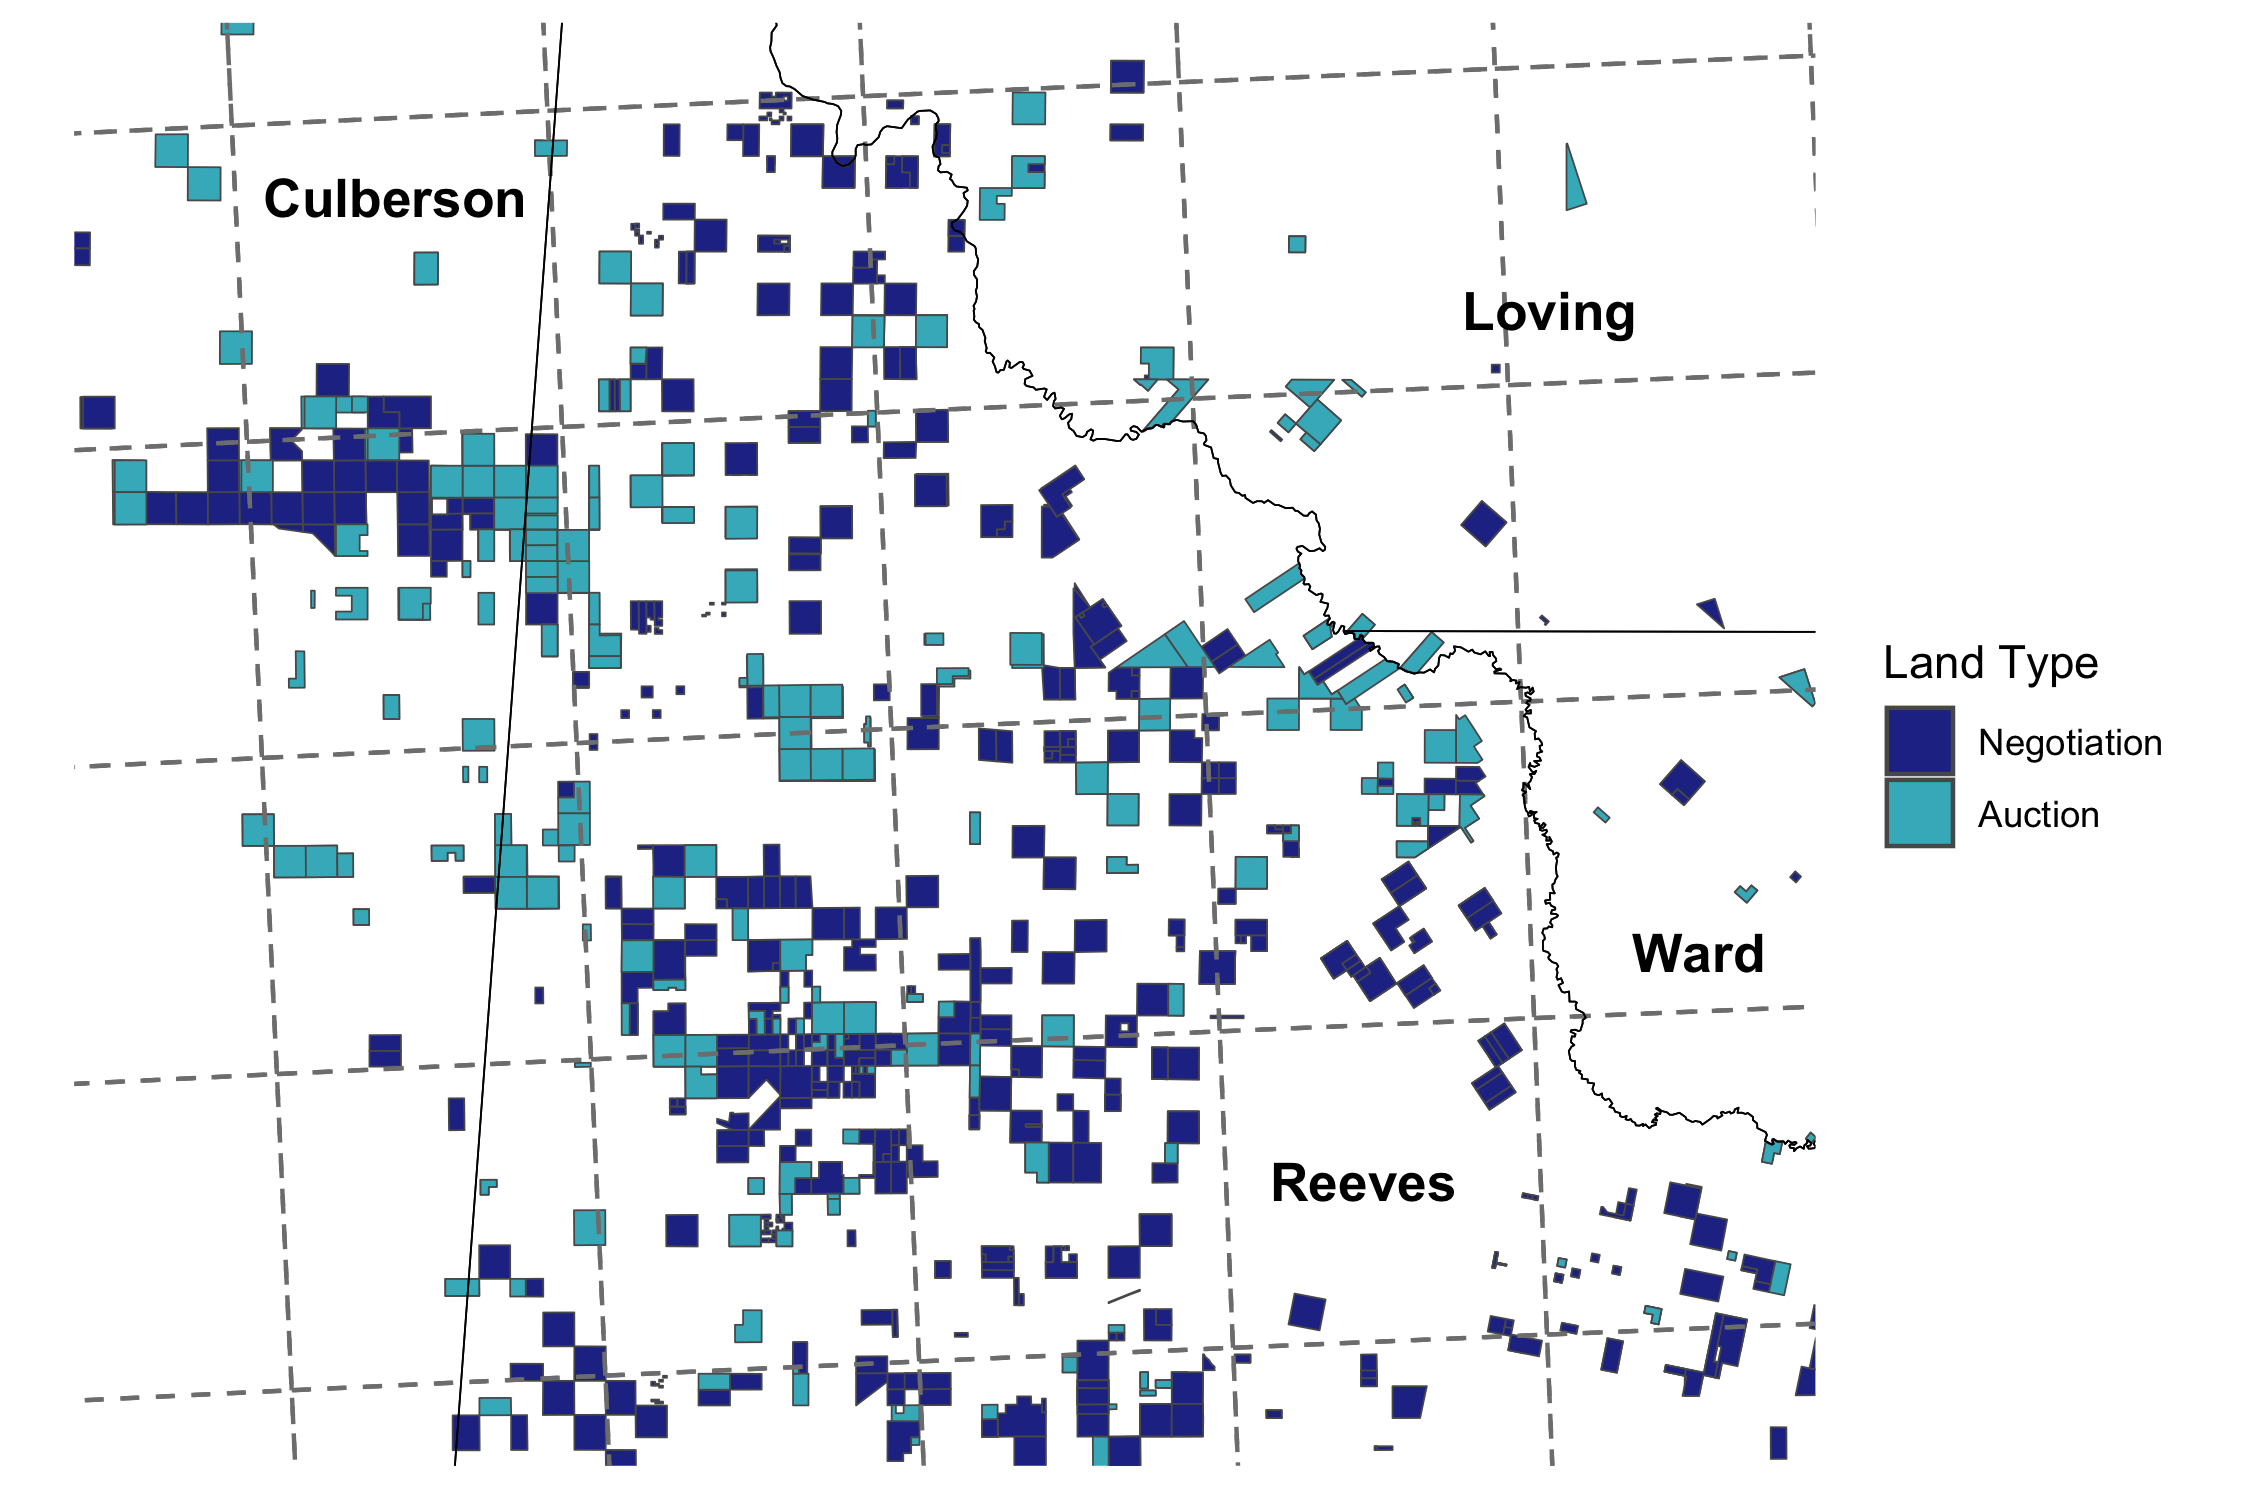
\includegraphics[width=.9\textwidth]{../output/figures/sample_glo_leases.png}
	\par\end{centering}
\end{figure}

There is no \textit{a priori} sense in which a given fixed effect specification correctly controls for the effects of unobserved quality and market conditions on lease outcomes, and, as Figure \ref{fig:RAL_overlap_map} demonstrates, the grid boundaries we draw are quite arbitrary. We thus estimate several fixed-effects specifications which vary the size of the grids and the extent to which we interact the fixed effects for time and space. We also non-parametrically control for location and time using a novel application of the double/debiased machine learning techniques (DML) developed in \cite{chernozhukov2018double}.\footnote{Specifically, we estimate a \cite{robinson1988root} style partially linear specification of equation \ref{eq:mainAuction}.  We follow the procedures recommended in \cite{chernozhukov2018double} (equation 3.5, theorem 3.2, definition 3.3, and equation 4.4), finding the value of $\tau$ that minimizes the ``cross-fitted'' empirical analogue of 
\begin{equation*}
	\mathbb{E}\left[\left(Y - \gamma(L,T,X) - \tau(D - \delta(L,T,X))\right)\left(D - \delta(L,T,X)\right)\right]
\end{equation*}
where $D = \text{Auction}$, $\gamma(l,t,x) = \mathbb{E}\left[Y\mid L = l, T = t, X = x\right]$, $\delta(l,t,x) = \mathbb{E}\left[D\mid L = l, T = t, X = x\right]$ and we estimate the functions $\gamma(\cdot)$ and $\delta(\cdot)$ using random forests.  For more details, see Appendix \ref{sec:dml}.} Both of these strategies ensure we are making comparisons between leases with similar mineral quality that transact at similar times. 

A final concern with interpreting $\tau$ in equation \ref{eq:mainAuction} as the causal effect of auctioning vs. negotiating a mineral lease is that the data, by construction, is restricted to successful transactions. However, in both mechanisms it is possible that a potential transaction fails, leaving its parcel temporarily unleased. If the probability of a successful transaction varies across mechanisms, then this sort of selection will bias our estimate of $\tau$ for the reasons outlined in \cite{heckman1979sample}. Moreover, when transactions fail, the seller experiences zero revenue, and if failure is differentially likely between auctions and negotiations, then these zeros are a real part of the differences in seller welfare between the two mechanisms. 

We address this concern in two ways. First, we ask whether the two mechanisms generate leases at different rates, which is a necessary condition for selection to bias our estimate of $\tau$ in equation \ref{eq:mainAuction}. In Section \ref{sec:ResultsParcels} we show that the two mechanisms have statistically indistinguishable leasing rates for all but two of the fifty-two quarters in our lease sample. In Appendix \ref{app:duration}, we also show the two mechanisms have statistically indistinguishable hazard rates of lease formation. Second, in Section \ref{sec:ResultsParcels} we re-esimate equation \ref{eq:mainAuction} at the parcel level.  We compute parcel outcomes as the discounted sum of lease outcomes associated with each parcel, among the entire population of PSF parcels. Because this population includes parcels that never lease, these parcel level analyses are immune to the aforementioned selection concern.  Moreover, by studying the aggregate discounted outcomes on each parcel, these parcel level analyses directly capture the ``zero revenue'' extensive margin effects discussed above.  As we discuss in Section \ref{sec:ResultsParcels}, the parcel level results are qualitatively similar to the lease level results we report in \ref{sec:ResultsLease}. 

\section{Lease Results \label{sec:ResultsLease}}

\subsection{Bonus Results \label{subsec:ResultsLeaseBonus}}
We begin by investigating the impact of auctions on up-front payments, estimating several versions of equation \ref{eq:mainAuction} with the natural logarithm of bonus payments as the dependent variable. Table \ref{tab:table_main_bonus} presents the results.\footnote{In Appendix Table \ref{tab:table_main_bonus_levels} we report similar results in levels.} All models include controls for the size of the lease, in acres. In column 1, we include fixed effects for the year-quarter of the lease's effective date and for the 10 mile square grid containing the lease's centroid. The interpretation of this estimate is that auctioned leases generate \inputy{../output/estimates/Bonus_Grid10_log.tex} log points more in bonus payments than similar negotiated leases, and this difference is precisely estimated.\footnote{Note that in percentage terms, this difference considerably larger than \inputy{../output/estimates/Bonus_Grid10_log.tex}\%, as $\exp(0.55) - 1 \approx 73\%$. In appendix \ref{sec:extra_regressions}, we repeat these regressions in levels, with the dollar value of the bonus payments (per acre) as the left-hand side variable.}  In column 2, we interact the grid indicators with year of sample indicators, to account for the fact that different locations in Texas were developed at different times in our sample. Even with these interactive fixed effects, the estimated auction coefficient is stable, with auctions paying \inputy{../output/estimates/Bonus_Grid10Yr_log.tex} log points more, and is still precisely estimated. This model, which compares leases for minerals that are located at roughly the same place and which transact at roughly the same point in time, is our main specification. 

\addtolength{\tabcolsep}{2pt}
\begin{table}[htpb]
	\begin{center}
	\begin{threeparttable}
	\caption{Bonus Payments and Mechanism Type}
	\label{tab:table_main_bonus}
	\small
	
\begin{tabular}{lccccccccc}
\toprule
 & ( 1 ) & ( 2 ) & ( 3 ) & ( 4 ) & ( 5 ) & ( 6 ) & ( 7 ) & ( 8 ) & ( 9 )\\
\midrule
 & 0.55 & 0.53 & 0.44 & 0.52 & 0.58 & 0.53 & 0.58 & 0.58 & 0.59\\

\multirow{-2}{*}{\raggedright\arraybackslash Auction} & (0.06) & (0.06) & (0.08) & (0.07) & (0.05) & (0.06) & (0.05) & (0.10) & (0.08)\\

\midrule
Grid & 10 & 10 & 10 & 20 & DML & 10 & DML & 10 & DML\\

Time & Q & GY,Q & GYQ & GY,Q & DML & GY,Q & DML & GY,Q & DML\\

Extra & No & No & No & No & No & Yes & Yes & No & No\\

Private Only & No & No & No & No & No & No & No & Yes & Yes\\

N & 1,515 & 1,515 & 1,515 & 1,515 & 1,515 & 1,260 & 1,260 & 1,308 & 1,308\\

$R^2$ & 0.914 & 0.961 & 0.972 & 0.944 &  & 0.954 &  & 0.960 & \\
\bottomrule
\end{tabular}
            
	\footnotesize
		\begin{tablenotes}
			\item The dependent variable in each regression is the natural logarithm of bonus payments. In columns 1-4 and 6 and 8, the size of the location bins, in miles, are indicated in the ``Grid'' row, while the structure of the time controls (``Q'' for quarter of sample, ``GY,Q'' for grid-by-year plus quarter of sample, and ``GYQ'' for grid-by-quarter of sample) are indicated in the ``Time'' row.  Standard errors are clustered by grid in columns 1-4 and 6 and 8.  Columns 5, 7, and 9 use a double/debiased machine learning routine, as recommended in \cite{chernozhukov2018double}.  For estimation details, see Appendix \ref{sec:dml}.  ``Extra'' controls include shape regularity, a dummy variable for whether the lease spans multiple parcels, surface cover measures, distance to roads and water sources, and shale thickness, which is only available in the Permian Basin and parts of the Eagle Ford shale.  Fixed effect models include a spline in lease size and the DML model includes lease size as a random forest covariate.  The average negotiated bonus payment is \$\inputy{../output/estimates/negotiation_avg_bonus.tex} per acre.    
		\end{tablenotes}
	\end{threeparttable}
	\end{center}
\end{table}

In the next set of columns, we investigate the sensitivity of these results to alternative time-space controls. In column 3, we include location-quarter-of-sample fixed effects to impose more stringent limits on which leases can be compared over time.  To ensure that our results are robust to different choices of spatial controls, in column 4 we use 20 mile grids instead of 10 mile grids.  In both cases, the resulting estimates are nearly identical to the results in column 2.  In column 5, we replace the grid and time fixed effects with a non-parametric control for the lease's location and time using random forests in a double/debiased machine learning model (DML). Across all of these specifications, we find consistent evidence that bonus payments are substantially larger in auctions than they are in negotiations. Even at the lower end of these estimates, the implications for seller revenue are large.  For an RAL lease of average size, switching to an auction would generate a \$\inputy{../output/estimates/Bonus_Grid10Yr_log_total.tex} larger up-front bonus payment. 

As we discussed in Section \ref{sec:EmpiricalStrategy}, our key identifying assumption is that land which was initially owned by the state and sold by 1931 is similarly valuable for today's hydrocarbon exploration as land from the same allocation that was not sold before 1973. While we believe it is unlikely that the timing of early land transactions would be correlated with the productivity of shale formations that were unknown until the early 2000's, our empirical specifications include flexible spatial controls to account for any differences in geology across leases governed by the two mechanisms.  Moreover, Table \ref{tab:ParcelBalanceAll} shows that the two types of land are also indistinguishable along observable measures of quality that were known at the time the mechanism type for a parcel was determined.  However, even if the two parcel types were similar at the time the mechanism type was determined, by construction, they have been exposed to a different history of surface ownership.  RAL surface owners have had at least 73 years\footnote{Our lease sample starts in 2004, and the latest RAL privatization from the PSF was in 1931.} to develop their surface rights, while State auction parcels were privatized no more than 40 years ago, if ever. To the extent that surface investments help or hinder shale development, they would generate differences across parcel types in their value during the shale boom, even if a parcel's leasing mechanism (negotiation or auction) was as good as randomly assigned. 

To ensure that such differences do not confound our estimates, we estimate a series of additional specifications that include measures of surface quality related to subsequent surface investment.  Using our lease shape files, we compute the quality of the lease's shape as the ratio of its area to the area of the convex hull containing it and separately determine whether the lease spans more than one distinct parcel.  Next, we measure the distance of each lease to road infrastructure \citep{txdot}.  Finally, we compute the most common surface coverage characteristics of a lease \citep{nlcd}.\footnote{Table \ref{tab:ParcelBalanceAll} demonstrates that leases the parcels underlying our sample leases are statistically indistinguishable along these surface measures.}  In the remaining columns of Table \ref{tab:table_main_bonus}, we confirm that the bonus results above are robust to including these characteristics as controls. Columns 6 and 7 estimate the grid-year and DML models with additional controls for measures of surface quality, like the convexity of the lease's shape, an indicator for whether the lease spans multiple parcels, the distance from the lease to roads and water infrastructure, and satellite measures of the lease's landcover, as well as the thickness of the shale underlying the lease. Across all of these specifications, we continue to find that auctions pay significantly more than negotiations do.

One remaining potential confounder, which \emph{is} observably different across the two groups of leases, is surface ownership. The Relinquishment Act specifically allows a subset of private surface owners to perform negotiations, so all of our negotiated leases have private surface ownership. In contrast, some auctions occur on PSF parcels that were never sold, and as a result, have state surface ownership.  Private surface ownership itself could reduce the value of a negotiated lease if, for example, private surface owners have houses or livestock on their property, or if E\&P companies simply face additional constraints on drilling near private citizens, relative to leases where the state controls the surface. If these constraints made negotiated leases more difficult to develop, E\&P companies would rationally pay less to lease them, but this difference in payment would not be caused by the difference in mechanisms. This scenario would violate our exclusion restriction, as the difference in bonuses on RAL lands would come from the fact that they have private surface owners, not the manner in which they were allocated.

To ensure that our results are not driven by differences in private surface rights, we restrict our analysis to parcels where the state does not own surface rights. This constitutes leases on land that the State sold to private individuals after 1973, and excludes leases on land that still belong to the PSF.  If there are additional costs to developing leases with private surface ownership, we would expect the difference in bonus payments between these leases and leases on RAL parcels to be smaller than the overall difference we observe, when including the full set of auction leases. Columns 8 and 9 of Table \ref{tab:table_main_bonus} present our main bonus regressions estimated on this restricted sample. Despite the fact that these regressions exclude slightly more than half of all auctioned leases, the estimates are still consistent with the results in columns 1 and 5: both point estimates are statistically significant at conventional levels, and they comfortably lie within the confidence intervals for the estimates covering the entire sample.  We therefore reject the concern that negotiated leases earn lower bonus payments because they are associated with private surface ownership.

Finally, surface owners of RAL parcels sometimes negotiate additional contractual provisions which deviate from the standard RAL lease, and it could be the case that these additional contractual demands compensate RAL lessors for the lower bonus payments they receive.  To test this hypothesis, we collected and digitized data on the auxiliary clauses embedded in each RAL lease.  As we document in Appendix \ref{sec:Appendix_Addenda}, we find no evidence that variation in the number of additional contractual demands or the relative landowner vs. E\&P company ``friendliness'' of those contractual demands can explain the differences in bonus payments that we observe.   Even after conditioning on these additional contractual characteristics, auctioned leases still pay considerably higher bonus payments than negotiated leases do.

\subsubsection*{Other Lease Terms \label{subsec:ResultsLeaseChars}}
As we noted in Section \ref{sec:MineralBackground}, all leases are three-part contracts: bonus, royalty, and primary term. While the previous analysis shows that auction bonuses are higher, it could be that RAL leases are compensated for this difference in up-front payments with higher royalties, or shorter terms.\footnote{Note that the \textit{equilibrium} effect of higher royalties and/or shorter terms need not actually increase the value that a landowner gets from a lease, due to the moral hazard issues explored in \cite{herrnstadt}.  Higher royalties and shorter primary terms may reduce the chance the lessee actually drills.} In Table \ref{tab:royalty_term_stacked}, we estimate regressions in which royalty and primary term are the left-hand side variable.  Across these specifications, auctions generate leases with higher royalty rates, by about 1 percentage point, and longer primary terms, by about 1 year.  

\addtolength{\tabcolsep}{4pt}
\begin{table}[htpb]
	\begin{center}
	\begin{threeparttable}
	\caption{Royalty Rates, Primary Terms, and Mechanism Type}
	\label{tab:royalty_term_stacked}
	\small
	
\begin{tabular}{lccccc}
\toprule
  & ( 1 ) & ( 2 ) & ( 3 ) & ( 4 ) & ( 5 )\\
\midrule
 & 0.95 & 0.86 & 0.90 & 0.86 & 0.82\\

\multirow{-2}{*}{\raggedright\arraybackslash Auction - Royalty Rate} & (0.13) & (0.17) & (0.25) & (0.14) & (0.09)\\

$R^2$ & 0.540 & 0.752 & 0.846 & 0.683 & \\

\midrule
 & 1.00 & 0.86 & 0.85 & 0.87 & 0.99\\

\multirow{-2}{*}{\raggedright\arraybackslash Auction - Primary Term} & (0.10) & (0.10) & (0.13) & (0.09) & (0.05)\\

$R^2$ & 0.521 & 0.732 & 0.835 & 0.641 & \\

\midrule
Grid & 10 & 10 & 10 & 20 & DML\\

Time & Q & GY,Q & GYQ & GY,Q & DML\\

N & 1,515 & 1,515 & 1,515 & 1,515 & 1,515\\
\bottomrule
\end{tabular}
            
	\footnotesize
		\begin{tablenotes}
			\item The dependent variable in the top row is the lease's royalty rate, in percentage points.  The dependent variable in the bottom row is the lease's primary term in years. In columns 1-4, the size of the location bins, in miles, are indicated in the ``Grid'' row, while the structure of the time controls (``Q'' for quarter of sample, ``GY,Q'' for grid-by-year plus quarter of sample, and ``GYQ'' for grid-by-quarter of sample) are indicated in the ``Time'' row.  Standard errors are clustered by grid in columns 1-4.  Column 5 uses a double/debiased machine learning routine, as recommended in \cite{chernozhukov2018double}.  For estimation details, see Appendix \ref{sec:dml}.  Fixed effect models include a spline in lease size and DML models include lease size as a random forest covariate.      
		\end{tablenotes}
	\end{threeparttable}
	\end{center}
\end{table}
\addtolength{\tabcolsep}{-2pt}

Given these two facts, it is natural to question how much higher bonuses are \emph{conditional} on these other lease characteristics. However, royalty rates and primary terms are determined by the mechanism of interest, so a regression that included them as right hand side variables would not have a causal interpretation.\footnote{This is an example of what \citet{angrist2008mostly} term ``bad controls.''} To the extent that higher royalties and/or longer primary terms in auctions make lessors better or worse off, we will capture these effects in the next section, where we examine production, royalty revenues, and total seller revenues, in the same causal framework we use here.  For completeness, we also report the results of bonus regressions that include a lease's royalty rate and primary term as right hand side variables in Appendix Table \ref{tab:BonusWithRoyaltyTerm}.  The coefficients on the auction dummy, while lacking a causal interpretation, are precisely estimated and similar in magnitude to what we report in this section. 

\subsection{Allocative Efficiency Results \label{sec:ResultsProductivity}}

One potential explanation for the large difference in bonus payments between auctions and negotiations is that auctions select more productive firms, and these firms are correspondingly willing to pay more for the option to drill. As we discussed in Section \ref{sec:MineralBackground}, there are many sources of productivity differences across E\&P companies. Auctions could select better firms by attracting more bidders than negotiations do, or by simply better identifying the best bidder from the same set that participate in negotiations.\footnote{Given that property rights are well defined here, and typically transferable, one might think that any initial misallocation by negotiators would be quickly rectified through secondary markets. However, even absent any transaction costs, asymmetric information between the initial lessee and a potentially more productive alternative lessee will prevent many socially beneficial reassignments. For a theoretical review of informational frictions and the Coase Theorem, see \citet{Farrell1987-df}. \cite{BrehmLewis} provide compelling empirical evidence on this point in the specific case of mineral leasing.} If this were true, we'd expect auctions to not only pay more than negotiations, they ought to produce more, as well.  Alternatively, auctions and negotiations might select equally productive firms, but the absence of formality in negotiations and/or greater competition in auctions allows negotiation winners to pay less than auction winners do.  Under this hypothesis, we'd expect auctioned and negotiated leases to produce at similar levels, and the difference in bonus payments that we observe would simply reflect a shift in the division of surplus between firms and landowners. To distinguish between these two theories, we measure the differences in realized output between auctioned and negotiated leases. 

We begin by looking at differences in production revenues, as recorded in GLO administrative data. Lessees make monthly royalty payments to GLO. We divide these payments by the associated royalty rate to infer the total revenues generated by a lease during a month, then discount the observed stream of monthly revenue back to the lease's effective date.  We call this measure \textit{lease revenue}, as it represents the total production revenue that the lease generates.  Though our data covers all production through March, 2019, leases are expected to produce output for 20 years or more. This means that the discounted sum of realized revenue is right censored, even for the earliest cohort of leases. To remove some of the bias due to censoring on the extensive margin, we restrict our analyses output and lease revenues to leases whose primary term has concluded by the end of our royalty data, the last of which was signed in 2013. We also include the same temporal controls as in the bonus regressions, to ensure that we are making comparisons between auctioned and negotiated leases that are at least similarly censored.  

Table \ref{tab:output_stacked} presents the results. Focusing first on panel (a), the first five model specifications are identical to those in Table \ref{tab:table_main_bonus}, showing the effects of mechanism type on each output measure under various spatial and temporal controls.  The final column is similar to the specification in column 1 of Table \ref{tab:BonusRobust}, and surface characteristic controls.  Across these specifications, auctioned leases produce \$\inputy{../output/estimates/lease_rev_min.tex} to \$\inputy{../output/estimates/lease_rev_max.tex} more in lease revenue, per acre. Though the point estimates are somewhat imprecise in specifications with finer fixed effects or additional covariates, they are consistently large, and represent an economically significant difference in output, relative to the average lease revenues from negotiated leases of \$\inputy{../output/estimates/negotiation_avg_revenue.tex} per acre. 

\addtolength{\tabcolsep}{4pt}
\begin{table}[htpb]
	\caption{Lease Revenue, Lease Output, Seller Revenue, and Mechanism Type \label{tab:output_stacked}}
	\begin{threeparttable}
	\small
	\subfloat[Linear Regression Models]{
\begin{tabular}{lcccccc}
\toprule
  & ( 1 ) & ( 2 ) & ( 3 ) & ( 4 ) & ( 5 ) & ( 6 )\\
\midrule
 & 3.47 & 2.64 & 2.61 & 3.60 & 4.56 & 2.91\\

\multirow{-2}{*}{\raggedright\arraybackslash Auction - Lease Revenue} & (1.28) & (1.43) & (2.76) & (1.23) & (1.60) & (1.52)\\

\midrule
 & 0.85 & 0.82 & 0.92 & 1.03 & 1.13 & 0.93\\

\multirow{-2}{*}{\raggedright\arraybackslash Auction - Output} & (0.31) & (0.40) & (0.73) & (0.30) & (0.38) & (0.42)\\

\midrule
 & 1.41 & 1.15 & 1.30 & 1.46 & 1.89 & 1.22\\

\multirow{-2}{*}{\raggedright\arraybackslash Auction - Seller Revenue} & (0.36) & (0.39) & (0.72) & (0.35) & (0.43) & (0.42)\\

\midrule
Grid & 10 & 10 & 10 & 20 & DML & 10\\

Time & Q & GY,Q & GYQ & GY,Q & DML & GY,Q\\

Extra & No & No & No & No & No & Yes\\

N & 1,259 & 1,259 & 1,259 & 1,259 & 1,259 & 1,012\\
\bottomrule
\end{tabular}
} \\
	\subfloat[Pseudo-Poisson Regression Models]{\input{../output/tables/stacked_output_Poisson.tex}}
		\begin{tablenotes}
		\footnotesize
		\item The dependent variables are the discounted sum of oil and gas production revenue (Lease Revenue), in thousands of dollars, discounted barrels of oil equivalent (Output), in hundreds, and the discounted present value of the sum of bonus payments, delay rentals paid, fees and production royalties (Seller Revenue), in thousands.  In the top panel, the estimates come from linear regression models, with outcomes per acre, while in the bottom panel, they come from pseudo-Poisson quasi-maximum likelihood models, with outcomes in levels.  In both panels, the estimates use fixed effects in columns 1-4 and 6, where the size of the location bins, in miles, are indicated in the ``Grid'' row, and the structure of the time controls (``Q'' for quarter of sample, ``GY,Q'' for grid-by-year plus quarter of sample, and ``GYQ'' for grid-by-quarter of sample) are indicated in the ``Time'' row.  For these models, standard errors are clustered by grid.  In both panels, column 5 uses a double/debiased machine learning routine, as recommended in  \cite{chernozhukov2018double}.  For estimation details, see Appendix \ref{sec:dml}.  The fixed effect models include a spline in acres, while the DML models include acres as a covariate in the random forest routine. ``Extra'' controls include shape regularity, a dummy variable for whether the lease spans multiple parcels, surface cover measures, distance to roads and water sources, and shale thickness, which is only available in the Permian Basin and parts of the Eagle Ford shale.  The sample includes all leases whose primary term ends before March, 2019.  In the fixed effect models of columns 1-4 and 6 in the bottom panel, the leases from grids and/or time periods with no variation in output are dropped, as the outcome is completely determined.  The average negotiated lease generates \$\inputy{../output/estimates/negotiation_avg_revenue.tex} in lease revenue per acre, and \inputy{../output/estimates/negotiation_avg_dboe.tex} of discounted barrels of oil equivalent per acre.    
		\end{tablenotes}	   
	\end{threeparttable}
\end{table}
\addtolength{\tabcolsep}{-4pt}

Although landowners ultimately care about production revenues (the product of quantities and prices), E\&P companies have little ability to influence the prices at which these commodities sell.  As a result, variation in output may better capture the traditional notion of productivity differences between auction and negotiation winners than variation in revenues does.\footnote{For a review of this literature, see \cite{syverson2011determines}.}  In consideration of this, we divide our product specific production revenue data by contemporaneous oil and gas prices, and define \textit{output} as the sum of these two series, weighing gas production by its energy content in barrels of oil equivalent terms.\footnote{We assume 1,000 cubic feet of natural gas production is equivalent to 0.1767 barrels of oil production, per EIA guidelines here: \url{https://www.eia.gov/tools/faqs/faq.php?id=45&t=8}}  We then estimate the same set of specifications using output per acre as the left hand side variable, which we report in the second row in the top panel of Table \ref{tab:output_stacked}. Across specifications, auctioned leases produce \inputy{../output/estimates/dboe_min.tex} to \inputy{../output/estimates/dboe_max.tex} additional discounted barrels of oil equivalent, per acre. These estimates are also more precise than the revenue estimates, because they are not affected by variation in prices over time. 

The statistical imprecision in some of these estimates may be driven by the fact that the distribution of both output and revenue, even normalized by lease size, is incredibly skewed. For leases that are ever drilled, the difference between the $10^{\text{th}}$ and $90^{\text{th}}$ percentiles of output per acre spans nearly three orders of magnitude. If all leases were drilled, a natural solution to this skewness would be to estimate differences in revenue and output across leases in relative terms, by using the natural logarithm of these terms as the dependent variables. However, fewer than half of leases are ever drilled, and as such generate zero revenue and output in the real sense (i.e., this is not just a selection problem).  In this situation, adding a small constant to these zeros to facilitate the logarithmic transformation is unlikely to be innocuous.  To make relative comparisons which respect this skewness, and to control for variation across cohorts in the extent of right-censoring, which we expect to have proportionate effects,\footnote{Log or Poisson style models will exactly control for censoring under an assumption that lease output declines at a constant proportional rate over time, a common assumption in petroleum engineering called ``Arps decline curve analysis.''} we also estimate pseudo-Poisson regression models, which effectively project the logarithm of the expected value of lease revenue (or output) onto mechanism type, covariates, and our location and time controls:
\begin{equation*}
 	\log \mathbb{E}\left[Y\mid \text{Auction}_i, X_i, L_i, T_i\right] = \tau \text{Auction}_i + X_i \beta + \delta_{L_i,T_i}. \label{eq:mainAuctionPoisson}
\end{equation*} 

The bottom panel of Table \ref{tab:output_stacked} presents the same specifications estimated using pseudo-Poisson regression models.  Because pseudo-Poisson models are not identified within grids and grid-time combinations that have no variation in output, the fixed-effect estimates drop data from some grids and times.  As a result, the pseudo-Poisson estimates in different fixed effect specifications are derived from slightly different samples, most of which are smaller than what we report in the top panel.  In spite of this, across specifications, we find consistent and mostly precisely estimated evidence that auctioned leases produce more than negotiated leases do.  Whether we use lease revenue or output as the outcome, auctions produce \inputy{../output/estimates/poisson_output_min.tex} to \inputy{../output/estimates/poisson_output_max.tex} log points more than negotiated leases do.  These results do not depend on how we control for location and time, nor whether we include additional covariates.\footnote{We showed in Section \ref{sec:ResultsLease} that auction leases have higher royalty rates than negotiation leases do.  Because higher royalty rates reduce firms' incentives to drill and invest in production, failure to control for royalty rates would cause us to underestimate the impact of auctions on output, all else equal. 

However, as discussed above, royalty rates are determined after assignment. To retain a causal interpretation in our regressions, we can only condition on royalty rates if we additionally assume that they are determined independently of the mechanism type. In Appendix Table \ref{tab:OutputWithRoyaltyTerm} we show, under this assumption, these differences in output are even higher when we condition on lease royalty rates and primary terms. If royalty rates \emph{were} determined independently of the mechanism type, this would imply that the results Table \ref{tab:output_stacked} are in fact underestimates of the true effect of auctions on output.

In Appendix Tables \ref{tab:drilledregs} and \ref{tab:outputconddrilled} we also show that these differences in output likely come from both the fact that auction leases are more likely to be drilled \emph{and} the fact that they produce more conditional on drilling. However, we caution that this decomposition does not have a causal interpretation because we do not have an instrument for drilling.} 

The combined effects of higher bonus payments and more production imply that auctions generate substantially more net benefit for sellers than negotiations do.  We measure this in the ``Seller Revenue'' rows of Table \ref{tab:output_stacked}, which use the discounted sum of bonus payments, discounted royalty revenues, and other fees as the dependent variable.  Auctions generate  \$\inputy{../output/estimates/sellerrev_min.tex} to \$\inputy{../output/estimates/sellerrev_max.tex} more revenue per acre for landowners than the negotiations do.  Under our main specification (column 2), this difference is worth about \$\inputy{../output/estimates/SellerRevenue_Grid10Yr_total.tex} for the average RAL lease.  These results show that auctions have an economically enormous impact on sellers.

\section{Parcel Results \label{sec:ResultsParcels}}

The results in Section \ref{sec:ResultsLease} show that auctioned leases pay and produce more than negotiated leases do. However, as discussed in Section \ref{sec:EmpiricalStrategy}, it is possible that a parcel's lease mechanism also affects the probability that a lease is signed at all. If this is the case, then a comparison of auctions vs. negotiations must account for the missing leases that didn't happen in one mechanism but would have under the other. In this section, we examine outcomes that occur at the parcel level. 

\subsection{Extensive Margin \label{sec:ExtensiveMargin}}
We begin our analysis of parcel outcomes by comparing the incidence of successful lease transactions on auction and negotiation parcels.  For auction parcels, we can directly compute the probability of a successful transaction, because we observe the list of parcels available in each auction event, as well as the subsequent bids.\footnote{Among GLO auctions on PSF land, \inputy{../output/estimates/tract_date_leased_share.tex}\% of nominated parcels failed to receive a qualifying bid, so on a per potential transaction basis, failure is quite common.  The GLO often offers to sell these failed parcels again in future auctions, to the point that \inputy{../output/estimates/tract_ever_leased_share.tex}\% of all observed nominated parcels transact \textit{at some point} in our sample.} However, we don't observe attempted negotiations that fail, so on negotiation parcels, we observe neither the likelihood of nomination nor the probability of a successful transaction after being nominated. In lieu of this, we use the linked parcel-lease data to directly look for differences in the extent to which a parcel is leased under the two mechanisms, inclusive of both differences in the likelihood of nomination and transaction success given nomination.  

To analyze this, we project a dummy indicating that a parcel is under lease in a given quarter onto an indicator for auction, as well as size and location controls. Figure \ref{fig:monthplot} provides a visual representation of the results. Though auction parcels are somewhat more likely to be under a lease in most quarters, the individual point estimates are quite noisy.  For all but 2 quarters, we cannot reject the hypothesis that auction and negotiation parcels are equally likely to be under a lease. As a result, we conclude that the two mechanisms do not differentially select parcels into leasing, and that the difference in outcomes between auctioned and negotiated leases is not due to a difference in the likelihood of transaction.\footnote{In appendix \ref{app:duration} we further explore this possibility with a formal duration analysis.  Specifically, for each parcel, we identify ``unleased spells,'' or periods during which a parcel has no active lease, and then ask whether RAL and State parcels in similar places, of similar sizes, that begin unleased spells at similar times, end their period of being unleased at similar rates.   Our analyses show that we cannot reject the hypothesis that unleased spells on RAL and State parcels end equally quickly.}

At first glance, the fact that auctions pay more but are no less likely to generate a successful transaction is perhaps surprising. However, this is explainable by two facts that we develop further below. First we show in section \ref{sec:Discussion} that the most active firms in our data participate in both mechanisms. Since there are no institutional restrictions on participation in either mechanism, it seems likely that nearby parcels allocated via different mechanism likely draw from the same distribution of bidders. Second, the same team that sets auction reserve prices at GLO also has final say over whether a negotiated transaction can take place, so it seems likely that the two mechanisms have similar reserve prices. Later on, in Table \ref{tab:AuctionRegs}, we show that while negotiated bids are much lower than nearby \emph{winning} auction bids, they are in fact higher than nearby reserve prices and statistically equivalent to the nearby minimum bid placed. If two mechanisms attract a similar distribution of bidders and also have similar ``reserve prices,'' the probability that at least one bidder has a value above the reserve price would be similar across the mechanisms. 

%\begin{figure}[!htbp]
\begin{figure}
    \centering
    \caption{Auctions and parcel leasing activity}
	\label{fig:monthplot}
	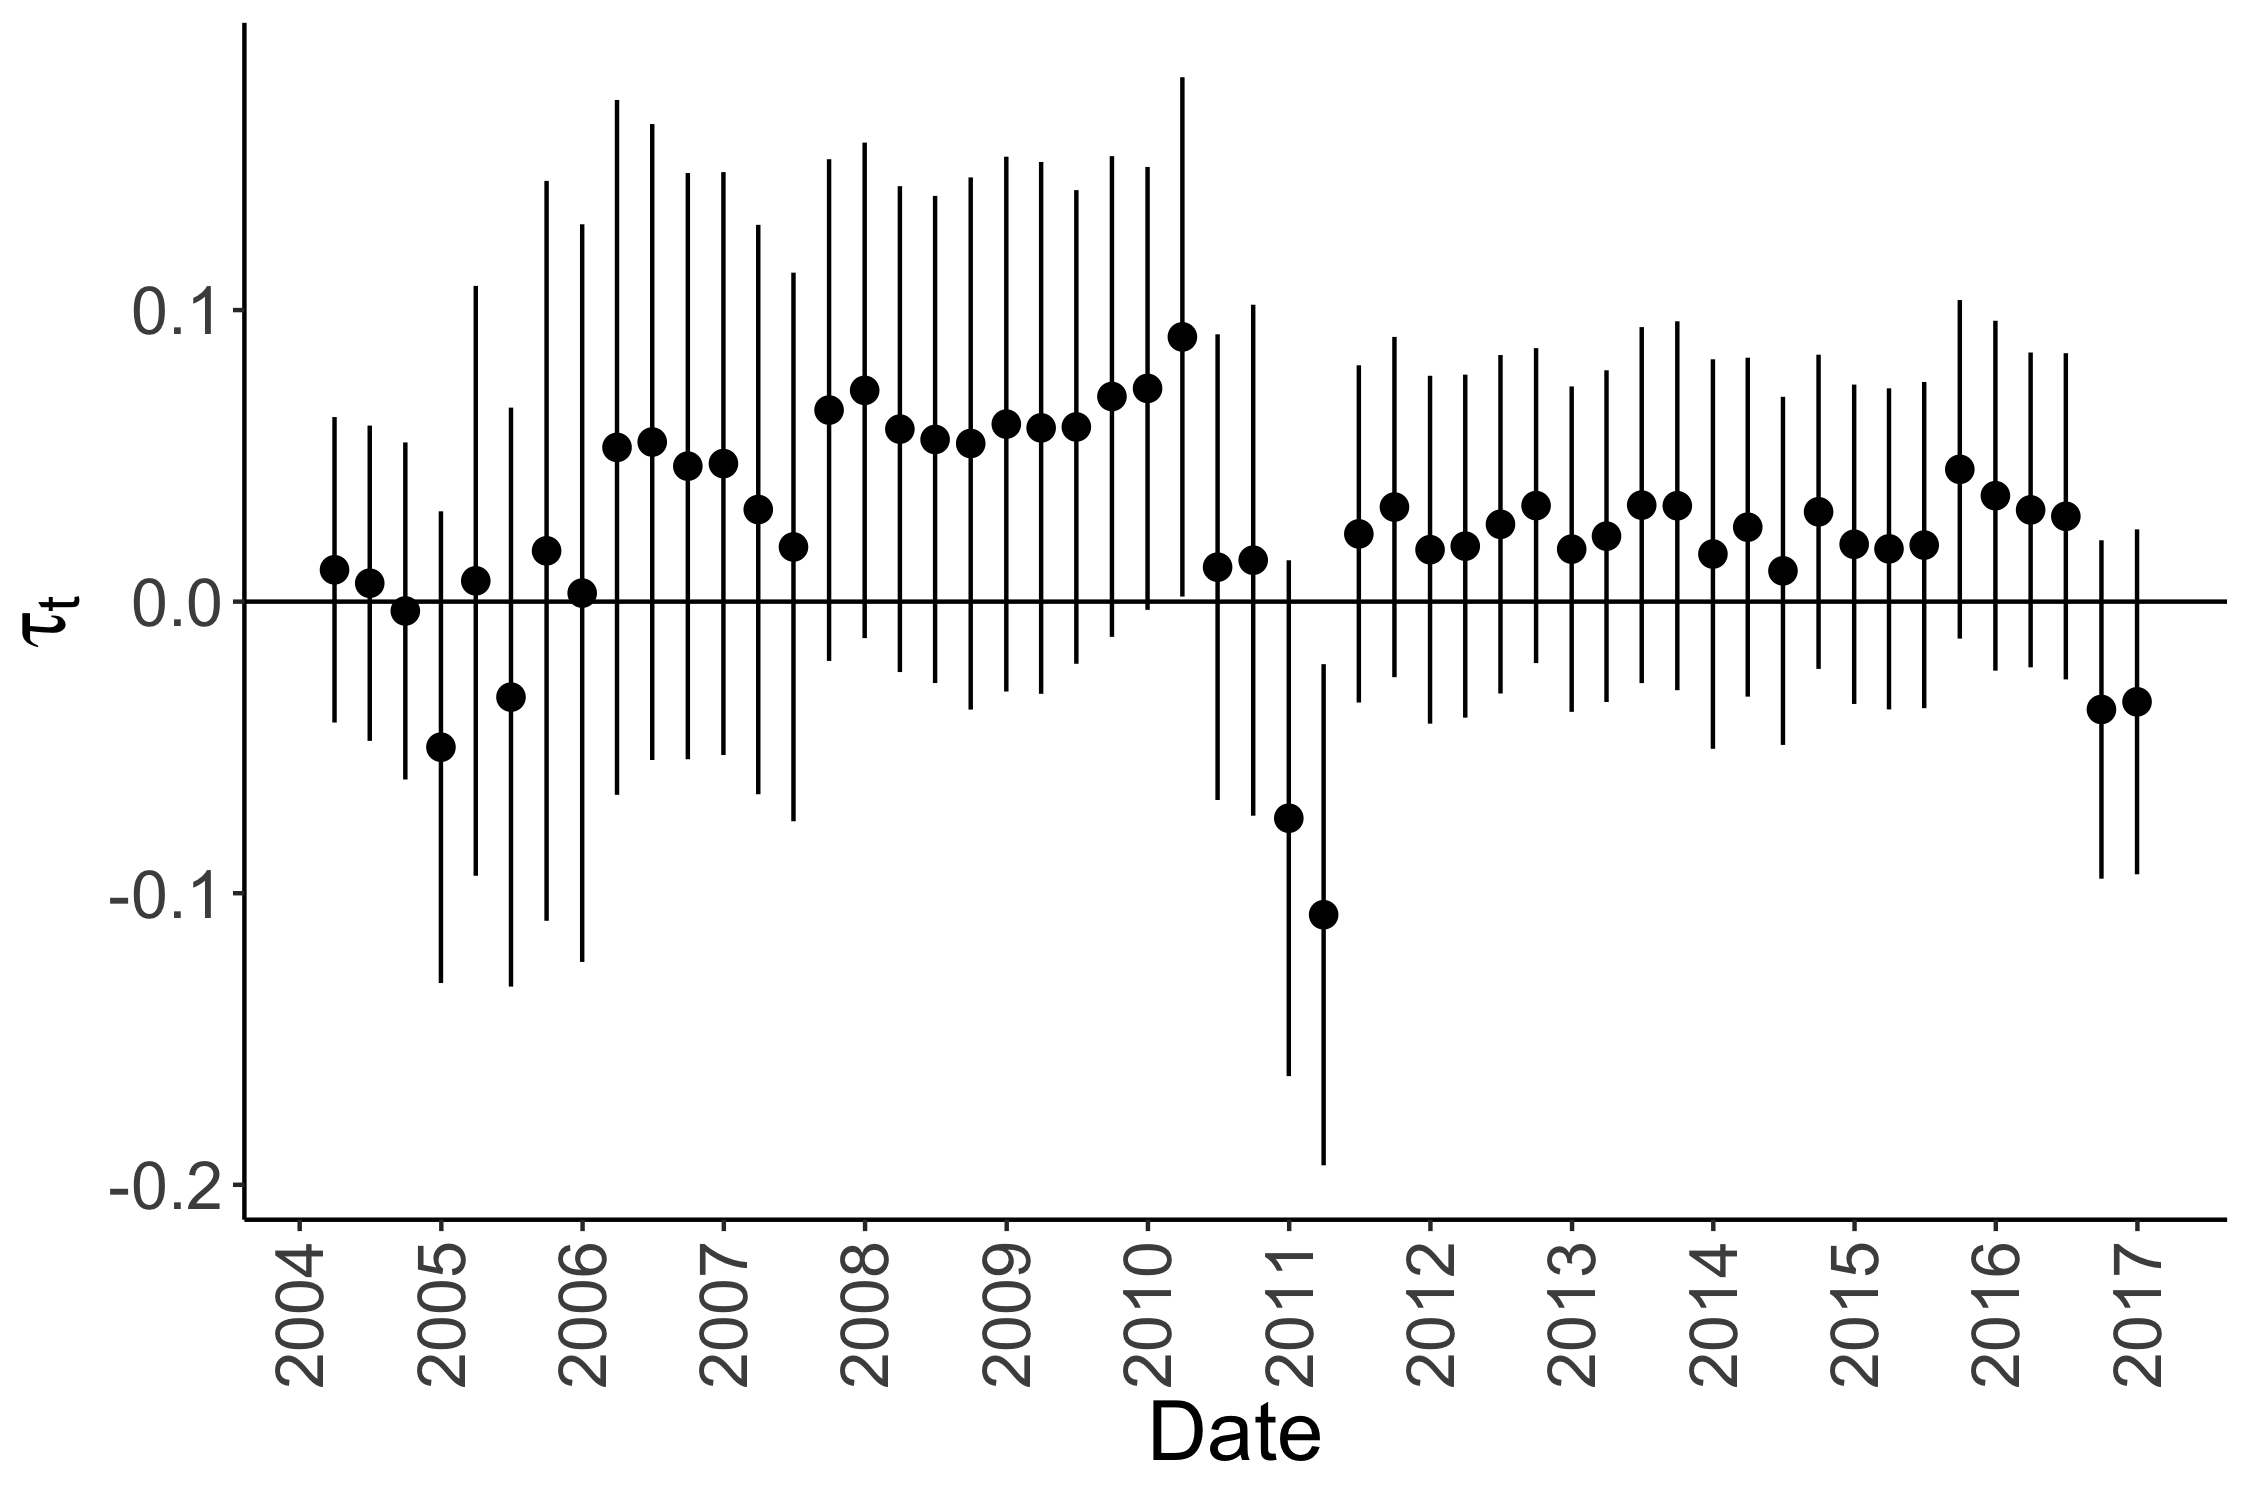
\includegraphics[width=.95\textwidth]{../output/figures/active_plot.png}
	\fignote{For each quarter between 2004-2016, we compute the effect of auction status on the likelihood that a parcel has any active leases.  We regress active status for parcel $i$ during quarter $t$ onto dummy equal to 1 for auction parcels and 0 for negotiatable parcels, parcel covariates, and Grid 10 fixed effects. 
		\begin{equation*}
	    	\text{Leased}_{it} = \tau_t \text{Auction}_i + X_i\beta + \delta_{l(i)} + \epsilon_{it}
	    \end{equation*}
  The figure shows point estimates and 95\% confidence intervals for each quarter's estimate of $\tau_t$, with standard errors clustered at the grid level.  A parcel is ``Leased'' if it has any active lease during a given quarter, including leases that were signed prior to 2004.}
\end{figure}

\subsection{Parcel outcomes \label{sec:ParcelOutcomes}}
We next look for differences in payment and production at the parcel level. As in Section 5, we restrict outcomes to those on leases signed between 2004 and 2013.\footnote{Although bonuses are not right censored, we restrict discounted bonuses here to leases signed by 2013 for consistency across parcel measures.} Table \ref{tab:ParcelOutcomes} presents the results. Like in our analysis of lease outcomes, we present two sets of models: linear regressions (per acre) and Poisson regressions. Across specifications, auction parcels earn about \$300 more per acre in discounted bonus payments in linear specifications and more than 60 log points more in Poisson specifications, and these differences are precisely estimated.  The differences in output and lease revenues are are all positive, and in most specifications are economically large.  While these estimates are precisely estimated in some Poisson specifications, the estimates in linear specifications are quite noisy. This is likely due to the additional zeros that come from parcels with no leases, and the skewness of output and lease revenue, conditional on leasing.  The combined effect of bonuses and royalty payments, reflected in the seller revenue models, suggests that auction parcels earn more that \$450 per acre than negotiation parcels.  In the Poisson models, the difference is 30 log points, or more. 

\begin{table}[htpb]
\begin{center}
\begin{threeparttable}
	\caption{Parcel Outcomes}
	\label{tab:ParcelOutcomes}
 	\small
   	
\begin{tabular}{lcccccc}
\toprule
  & ( 1 ) & ( 2 ) & ( 3 ) & ( 4 ) & ( 5 ) & ( 6 )\\
\midrule
 & 0.36 & 0.34 & 0.29 & 0.69 & 0.66 & 0.61\\

\multirow{-2}{*}{\raggedright\arraybackslash Auction - Bonus} & (0.08) & (0.10) & (0.04) & (0.08) & (0.10) & (0.06)\\

\midrule
 & 0.09 & 0.21 & 0.16 & 0.22 & 0.29 & 0.16\\

\multirow{-2}{*}{\raggedright\arraybackslash Auction - Output} & (0.16) & (0.15) & (0.12) & (0.14) & (0.10) & (0.12)\\

\midrule
 & 0.23 & 0.58 & 0.63 & 0.20 & 0.26 & 0.13\\

\multirow{-2}{*}{\raggedright\arraybackslash Auction - Lease Revenue} & (0.62) & (0.57) & (0.44) & (0.14) & (0.11) & (0.12)\\

\midrule
 & 0.46 & 0.52 & 0.45 & 0.37 & 0.40 & 0.30\\

\multirow{-2}{*}{\raggedright\arraybackslash Auction - Seller Revenue} & (0.19) & (0.19) & (0.12) & (0.08) & (0.08) & (0.07)\\

\midrule
Estimate & G10 & G20 & DML & G10 & G20 & DML\\

Estimator & Linear & Linear & Linear & Poisson & Poisson & Poisson\\

N & 2,621 & 2,621 & 2,621 & 2,132 & 2,240 & 2,621\\
\bottomrule
\end{tabular}
            
    \footnotesize
    \begin{tablenotes}
    	\item Columns 1-3 present ordinary least squares estimates of parcel level outcomes, \textit{per acre}, while columns 4-6 show pseudo-Poisson maximum likelihood estimates of aggregate parcel outcomes in levels.  Linear and Poisson fixed effect models include a spline in parcel size, while parcel size is part of the random forest covariates in both linear and Poisson DML models.  Bonus measured in thousands of discounted dollars, BOE measured in hundreds of discounted barrels of oil equivalent, lease revenue measured in thousands of discounted dollars, and seller revenue in thousands of discounted dollars.  All outcomes are discounted to January 1, 2004.
    \end{tablenotes}
\end{threeparttable}
\end{center}
\end{table}

These parcel results confirm the main takeways from Section \ref{sec:ResultsLease}: auction parcels pay lessors more and produce more output than negotiation parcels. However, the parcel results are generally smaller than the lease level results, and are considerably noisier. There are several reasons for this. First, many parcels never lease. While the previous section demonstrated that leasing was equally likely across parcel types, the parcel regressions still average in nearly thirty percent more zeros than the lease regressions. Second, the parcel regressions also include outcomes on leases that are excluded from the sample in Section \ref{sec:ResultsLease}. In our lease level analyses, we drop negotiated leases with features that do not overlap with auction leases, such as being too big or too small, or having multiple ownership interests. However, these lease level features are not defined at the parcel level, so we include these leases here. Third, even when leases are included in both samples, they may be weighted differently. When a lease spans two parcels, the outcomes from that transaction will get twice as much weight in a parcel level regression as a lease level regression. Conversely, if a single parcel has two leases on it, that parcel will effectively appear twice in the lease regressions but only once in a cross-sectional parcel regression. A final difference is the treatment of time. All lease regressions include quarter of sample fixed effects, to account for large changes in hydrocarbon prices and technology over time. However, the parcel regressions are inherently cross-sectional, with all outcomes discounted to 2004. In appendix \ref{app:lease-parcel-decomp}, we provide additional lease and parcel level regressions which remove some of these differences and provide more suitable comparisons. We find that a parcel-level regression restricted to parcels that ever lease yields results that are economically similar to, and often statistically indistinguishable from, a cross-sectional lease-level regression on the full population of leases. 

\section{Discussion \label{sec:Discussion}}

Auctioned leases pay and produce more than negotiated leases do. This is despite the fact that the land underlying auctioned and negotiated leases is nearly identical, as are the contracts governing the terms of investment and production. These differences in payment and output must therefore mean that auctions generate better matches than negotiations, in the sense that auctions allocate drilling rights to firms that value them more and can use them more productively.  In this section, we discuss the potential sources of heterogeneity in match value for a given piece of land, and assess the plausibility that these difference could generate such large gains in payment and output.

Thousands of E\&P companies operate in Texas, including more than 200 which produced more than 1,000 barrels of oil per day in 2020.\footnote{For firm-level production statistics, see \url{https://www.rrc.state.tx.us/oil-and-gas/research-and-statistics/operator-information/texas-oil-and-gas-producers-by-rank/}} Within this group, there are wide differences in size and observable measures of sophistication. Some of the largest publicly traded companies in the world, like Exxon and Chevron, compete for leases against a multitude of privately held E\&P companies with fewer than 20 employees.\footnote{For the firm size distribution in NAICS 20, Mining Quarrying \& Oil and Gas Extraction, for Texas, see \url{https://www.census.gov/data/tables/2017/econ/susb/2017-susb-annual.html}} Beyond observable differences in firm size and sophistication, there is also evidence for heterogeneity across firms in their engineering designs of hydraulic fracturing treatments, which are necessary for all leases in this setting \citep{bib:covert}. 

Given the many sources of vertical differentiation across firms, it is natural to ask whether auctions allocate to \textit{different} firms. Table \ref{tab:table_allocative} provides an answer, by tabulating auction and negotiation market shares for the ten most active lessees in our sample.\footnote{Firm identities in our data are recorded with some error (typos, etc). We describe our process for cleaning these names in Appendix \ref{sec:DataCleaning}.}  It is noteworthy that all but one of these large firms are active in both mechanisms, winning at least one auction and several negotiations each.\footnote{In further analysis of the auction bid data, we find that \inputy{../output/estimates/ever_bidder_negotiation_share.tex}\% of negotiated transactions are won by firms who place at least one bid at auction, and \inputy{../output/estimates/negotiation_winner_auction_share.tex}\% of auctions are won by firms that successfully complete at least one negotiation.}  Nevertheless, most firms have statistically and economically different shares of the auction and negotiation markets. The data soundly reject a $\chi^2$ test of the hypothesis that a firm's auction market share is the same as its negotiation market share  ($p<2\times 10^{-16}$).\footnote{$\chi^2$ tests of equal proportions for the top 20 and 40 most active lesses are similarly rejected.  Moreover, these differences in market shares across the mechanism types do not simply reflect differences in the distribution of a firm's ``interest'' across basins. We replicate this exercise within leases overlying the two largest shale basins in Texas, the Permian and the Eagle Ford, and can similarly reject a null hypothesis of equal proportions for the top 10 most active lessees in each basin.}  Thus, it does appear that the rate at which a firm wins a lease differs across auctions and negotiations.  

\begin{table}[htpb]
\begin{center}
\begin{threeparttable}
\caption{Auction and Negotiation Market Shares Among Active Lessees}
\label{tab:table_allocative}
 	\small
   	
\begin{tabular}{l>{\centering\arraybackslash}p{5em}>{\centering\arraybackslash}p{5em}>{\centering\arraybackslash}p{5em}>{\centering\arraybackslash}p{5em}}
\toprule
Firm & Leases & Auction Share & Negotiation Share & Overall Share\\
\midrule
CHESAPEAKE & 125 & 0.161 & 0.049 & 0.083\\
PETRO HUNT & 98 & 0.007 & 0.090 & 0.065\\
ENERGEN & 92 & 0.062 & 0.060 & 0.061\\
PETROHAWK & 72 & 0.084 & 0.032 & 0.048\\
SEGUNDO NAVARRO & 65 & 0.004 & 0.059 & 0.043\\
ANADARKO & 61 & 0.042 & 0.040 & 0.040\\
BP & 59 & 0.000 & 0.056 & 0.039\\
CIMAREX & 58 & 0.040 & 0.038 & 0.038\\
777 & 36 & 0.011 & 0.029 & 0.024\\
DEVON & 33 & 0.059 & 0.006 & 0.022\\
\midrule
ALL OTHERS & 816 & 0.531 & 0.542 & 0.539\\
\bottomrule
\end{tabular}
            
\end{threeparttable}
\end{center}
\end{table}

To assess whether this differential firm composition across mechanisms explains our results, we compare auctions and negotiations \textit{won by the same firm}.  Table \ref{tab:WithinFirm} shows estimates of our main bonus and output regressions, with and without fixed-effects for the identify of the firm that signed a lease.  Bonus payments, output, and lease revenue are larger on auctioned leases than negotiated leases, regardless of whether we condition on the identity of the winning firm.  In fact, point estimates for the within-firm gap between auction and negotiation outcomes are larger than than our baseline estimates for all three outcomes.  These results show that the large differences in payment and production between auctions and negotiations are not just the result of differences in the composition of firms who win auctions relative to negotiations. Auctions must also generate better \textit{horizontal} matches than negotiations do.  

\begin{table}[htpb]
	\begin{center}
	\begin{threeparttable}
	\caption{Effects of Firm Composition and Mechanism Type on Lease Outcomes}
	\label{tab:WithinFirm}
	\small
	
\begin{tabular}{lcccccc}
\toprule
 & Bonus & Bonus & Output & Output & Revenue & Revenue\\
\midrule
 & 0.53 & 0.58 & 0.821 & 1.583 & 2.64 & 4.67\\

\multirow{-2}{*}{\raggedright\arraybackslash Auction} & (0.06) & (0.08) & (0.403) & (0.681) & (1.46) & (2.07)\\

\midrule
Firm FE & No & Yes & No & Yes & No & Yes\\

N & 1,515 & 1,515 & 1,259 & 1,259 & 1,259 & 1,259\\

$R^2$ & 0.961 & 0.974 & 0.742 & 0.828 & 0.765 & 0.857\\
\bottomrule
\end{tabular}
    
		\begin{tablenotes}
			\footnotesize
			\item The dependent variable is the natural logarithm of the bonus payment (columns 1 and 2), discounted barrels of oil equivalent per acre (columns 3 and 4), or discounted lease revenue per acre (columns 5 and 6).  In columns 2-6, the sample includes all leases whose primary term ends before March, 2019.  All specifications include fixed effects for 10-mile grids-by-year and quarter-of-sample, as well as a spline in acres.   
			\end{tablenotes}        
	\end{threeparttable}
	\end{center}
\end{table}

There are many potential sources of horizontal heterogeneity in valuations for a drilling opportunity across firms, in the sense that firm A might be able to use lease X more productively than firm B, while B might be able to use lease Y more productively than firm A. For example, firms who already control acreage in the area may be able to develop a more efficient drilling plan. Firms who own hydrocarbon transportation infrastructure close to a given parcel may experience cost advantages in developing that specific parcel.  Similarly, firms with formation-specific knowledge about geology or efficient engineering choices will be able to produce more (or less expensively) than firms with less context-specific knowledge.

We can use auction bid data to measure the importance of such horizontal match quality across firm-lease pairs. GLO reports the bids submitted by all auction participants, not just the winner. Among large lessees, it is possible to observe the same two firms bidding against each other in many auctions.  If lease valuations were mostly vertical, in the sense that one firm was inherently more productive on all parcels than another, then the more productive firm would  reliably bid more than the less productive firm.  In contrast, if lease valuations were mostly driven by horizontal match quality, bid rankings would be less predictable. We check this in the bid data, by looking at all pairs of firms who bid in the same auction ten or more times.  Table \ref{tab:TopPairAuctionShares} lists these pairs and tabulates the probability that the alphabetically earlier firm (Firm A) bids more than the later firm (Firm B).  For 10 of the 12 pairs of firms, the fraction of the time that one firm wins more than the other is statistically identical to a coin toss, which strongly rejects the hypothesis that values are mostly vertical, at least among this set of firms.  To the extent that there are persistent vertical differences between firms, this data suggests that those are small relative to horizontal differences in firm-lease match values.  

\begin{table}[htpb]
	\begin{center}
	\begin{threeparttable}
		\caption{Bid ranking for top auction pairs}
		\label{tab:TopPairAuctionShares}
		\small
		
\begin{tabular}{llrrr}
\toprule
Firm A & Firm B & Auctions & Share A $>$ B & p-value\\
\midrule
CIMAREX & ENERGEN & 31 & 0.52 & 1.000\\
CIMAREX & CONOCOPHILIPS & 19 & 0.79 & 0.019\\
CIMAREX & RESOLUTE & 19 & 0.53 & 1.000\\
CONOCOPHILIPS & ENERGEN & 19 & 0.37 & 0.359\\
ENERGEN & RESOLUTE & 19 & 0.42 & 0.648\\
COG & RANGE & 17 & 0.41 & 0.629\\
CONOCOPHILIPS & RESOLUTE & 17 & 0.53 & 1.000\\
CIMAREX & MARSHFIELD OIL AND GAS LLC & 12 & 0.67 & 0.388\\
ENERGEN & MARSHFIELD OIL AND GAS LLC & 12 & 0.67 & 0.388\\
ADESCAPE INC & ENERGEN & 10 & 0.00 & 0.002\\
ADESCAPE INC & SEMEION RESOURCES LP & 10 & 0.30 & 0.344\\
ENERGEN & SEMEION RESOURCES LP & 10 & 0.80 & 0.109\\
\bottomrule
\end{tabular}
            
		\begin{tablenotes}
			\footnotesize
			\item $p$-value from a two-sided exact test of the hypothesis that the share of auctions in which Firm A bids more than Firm B is equal to 0.5, at a 95\% level.   
			\end{tablenotes}        
	\end{threeparttable}
	\end{center}
\end{table}

The previous discussion lays out several sources of heterogeneity in preferences for a lease across firms, and provides evidence that they exist in our sample.  Are these differences large enough to rationalize the large treatment effects we estimate? We can again use the auction bid data to answer this, using techniques from modern empirical auction analysis.

\addtolength{\tabcolsep}{-16pt}
\begin{table}[htpb]
\begin{center}
\begin{threeparttable}
	\caption{Auction Results by Number of Bidders}
	\label{tab:AuctionNBids}
 	\small
   	
\begin{tabular}{>{\centering\arraybackslash}p{6em}>{\centering\arraybackslash}p{6em}>{\centering\arraybackslash}p{6em}>{\centering\arraybackslash}p{6em}>{\centering\arraybackslash}p{6em}>{\centering\arraybackslash}p{6em}>{\centering\arraybackslash}p{6em}>{\centering\arraybackslash}p{6em}>{\centering\arraybackslash}p{6em}>{}p{6em}}
\toprule
Bids & Auctions & Average Reserve & Average Bonus & Average Reserve Margin & Average 1-to-2 Markup & Average 1-to-N Markup & Average 1-to-2 Allocative Gain & Average 1-to-N Allocative Gain\\
\midrule
1 & 252 & 704 & 1,325 & 0.54 &  &  &  & \\
2 & 97 & 860 & 1,790 & 0.71 & 0.38 &  & 0.50 & \\
3+ & 105 & 882 & 4,191 & 1.34 & 0.30 & 0.86 & 0.43 & 1.07\\
\bottomrule
\end{tabular}
            
    \footnotesize
    \begin{tablenotes}
    	\item This table summarizes bids from GLO auctions. The Bonus is the winning bid, in dollars per acre.  The ``Reserve Margin'' is the natural logarithm of the ratio of the winning bid to the reserve price.  The ``1-to-2 Markup'' is the natural logarithm of the ratio of the winning bid to the second highest bid, and the ``1-to-2-N Markup'' is the same, but comparing the highest and lowest bids.  The ``1-to-2 Allocative Gain'' is the natural logarithm of the ratio of the GPV pseudovalues of the winning and second highest bids, and ``1-to-N Allocative Gain'' is the same, but comparing the GPV pseudovalues of the highest and lowest bids.
    \end{tablenotes}
\end{threeparttable}
\end{center}	
\end{table}
\addtolength{\tabcolsep}{-2pt}

Table \ref{tab:AuctionNBids} summarizes the bid data from all \inputy{../output/estimates/tract_date_leased_insample.tex} GLO leases in our sample which cleared above the reserve. More than half of auctions receive only a single bid above the posted reserve price, and fewer than a quarter receive three or more bids.\footnote{During this time period, GLO auctions receive somewhat fewer bids per lease than neighboring New Mexico's state mineral auction does. The average successful auction in this sample has 2 bids.  In comparison, \cite{bhattacharya2018bidding} and \cite{kong_selective_2017} report 2.4 - 2.6 bids per auction in New Mexico.}  A key fact in this data is that winning bids are \textit{substantially} higher than non-winning bids, and regardless of how many bids an auction receives, those bids are quite a bit higher than reserve, even when there is no competition for the winner, \textit{ex post}.\footnote{\cite{kong_selective_2017} also observes this pattern in mineral lease auctions which take place in neighboring New Mexico, where the average single bidder auction transacts at \textit{seven} times the reserve price. Kong demonstrates that this behavior can be rationalized by bidder's having uncertainty about how much competition will show up to an auction.}  Moreover, winning bids are more than a little bit higher than losing bids.  For auctions with two or more bidders, the average winning bid is about 34 log points higher than the second highest bid, with smaller differences in auctions with three or more bidders.  The gap between winning bids and lower bids is even larger.  For auctions with three or more bidders, the difference between the winning bid and the \textit{lowest} bid is 86 log points, on average.  Thus, even when more than two bidders arrive at an auction, there are enormous differences in their apparent willingness-to-pay for the same property right. 

We can compare moments from the distribution of auction bids to our empirical estimates from sections \ref{sec:ResultsLease} and \ref{sec:ResultsParcels}. The average difference between negotiated and auction bonus payments in Table \ref{tab:table_main_bonus} is about 50 log points. This is close to the average reserve margin for auctions with just one bidder (54 log points), but smaller than the average across all auctions (76 log points). The highest 95\% upper confidence interval for the difference between auction and negotiation lease bonuses in Table \ref{tab:table_main_bonus} is only about 68 log points, so the average gap between auctions and negotiations is clearly smaller than the reserve margin. However this gap is larger than the average difference in bids between the highest and second highest bidder.\footnote{Note that these differences are constructed from \textit{within lease} comparisons, winning vs. losing bids for the same contract on the same piece of land, at the same point in time.  This difference is somewhat closer to the estimates in Table A.4, which compares auctions and negotiations that are both similar in location and time, \textit{and} have similar royalty rates and primary terms.} 

We can make this comparison between negotiated bonuses and losing auction bids explicit using regression. Table \ref{tab:AuctionRegs} repeats the log bonus regressions from Section \ref{sec:ResultsLease}, but replaces an auction's winning bid, which is its true bonus payment, with other bids placed for that lease (we do not modify negotiated bonus payments). The first two columns recreate the main results from Table \ref{tab:table_main_bonus}, showing that auctioned leases earn bonus payments that are 53-54 log points larger than similar negotiated bonus payments.  In columns 3 and 4, we replace realized auction bonuses with their reserve prices.  On average, auction reserve prices are somewhat \textit{lower} than negotiated bonus payments on leases that transact at similar places and times, which means that the core bonus payment result cannot be explained by negotiated leases frequently transacting at prices below the minimum level allowed in nearby auctions.  Columns 5 and 6 take this one step further, replacing auction bonuses with the minimum bid received.\footnote{For auctions with 1 bid, we define the minimum bid as the reserve price.}  In this comparison, we see that negotiations earn bonus payments that are similar, on average, to the lowest payment in nearby auctions.  Finally, columns 7 and 8 replace the auction bonus with the second highest bid.  Overall, these results are consistent with the results in Table \ref{tab:AuctionNBids}.  Negotiated transactions occur a prices above the reserve prices of auctions for similar leases, but at or slightly below the the second highest bid in those auctions. 

\addtolength{\tabcolsep}{15pt}
\begin{table}[htpb]
\begin{center}
\begin{threeparttable}
	\caption{$\log(\text{Bonus})$ results under alternative auction payment assumptions}
	\label{tab:AuctionRegs}
 	\small
   	
\begin{tabular}{lcccccccc}
\toprule
 & ( 1 ) & ( 2 ) & ( 3 ) & ( 4 ) & ( 5 ) & ( 6 ) & ( 7 ) & ( 8 )\\
\midrule
 & 0.53 & 0.58 & -0.14 & -0.07 & 0.00 & 0.06 & 0.10 & 0.15\\

\multirow{-2}{*}{\raggedright\arraybackslash Auction} & (0.06) & (0.05) & (0.04) & (0.04) & (0.05) & (0.04) & (0.06) & (0.05)\\

\midrule
Auction Bonus & Winner & Winner & Reserve & Reserve & Worst & Worst & Second & Second\\

Grid & 10 & DML & 10 & DML & 10 & DML & 10 & DML\\

Time & GY,Q & DML & GY,Q & DML & GY,Q & DML & GY,Q & DML\\
\midrule

N & 1,515 & 1,515 & 1,515 & 1,515 & 1,515 & 1,515 & 1,515 & 1,515\\
\bottomrule
\end{tabular}
            
    \footnotesize
    \begin{tablenotes}
    	\item ``Winner'' means auction leases get their actual bonus payment (the winning bid).  ``Reserve'' means auction leases get the reserve price instead of the winning bid.  ``Worst'' means auction leases get the worst price among all submitted bids, or the reserve price if only 1 bid was submitted.  ``Second'' means auction leases get the second best price among all submitted bids, or the reserve price if only 1 bid was submitted.  Fixed effect specifications include a spline in acres, while DML specifications include acres in the random forest component.
    \end{tablenotes}
\end{threeparttable}
\end{center}	
\end{table}
\addtolength{\tabcolsep}{-8pt} 

We can infer the underlying lessee values associated with these auction bids using a procedure similar to \cite{roberts2013unobserved}.\footnote{See Appendix \ref{sec:AppendixAuction} for implementation details.}  In the second to last column of Table \ref{tab:AuctionNBids}, we compare the winner's value to the second highest bidder's value.  As in our analysis of the bids themselves, we see that there are large differences between winning and losing values. For auctions with two bidders, the winner's value is 50 log points higher than the second highest bidder's value is, on average, and while the gap is smaller for auctions with more bidders, which are about half the sample, it is still economically large in auctions with three or more bidders, at 43 log points.  The difference between highest and lowest values, in auctions with three or more bidders, is even larger, at 107 log points.

It is somewhat harder to compare the distribution of bidder values with our output results. Bidders care about production that is expected to occur long after our royalty revenue data ends, so realized production may provide a negatively biased measure of bidder value.  On the other hand, bidders, as potential operators of mineral leases, also care about the costs of developing those leases, which we cannot measure with our output data.  Having noted those caveats, we compare the estimated allocative gains in the auction data with the results in Table \ref{tab:output_stacked}.  The 1-2 allocative gain, which is the average difference in log bidder values between the winner and second highest bidder, is well within the range of the point estimates in bottom panel of Table \ref{tab:output_stacked}.  Thus, an auction which mistakenly allocated a lease to the second highest bidder would suffer a decrease in allocative efficiency that is about as large as the differences in output that we estimate between similar auctioned and negotiated leases. However, the estimated output effects are considerably smaller than the average 1-N allocative gain.  

\addtolength{\tabcolsep}{10pt}

\subsection{Mechanism}

Mineral leases that are allocated by auction are better matched to E\&P firms than those allocated via negotiation. What features of negotiation process lead to worse matches? Unfortunately, we cannot answer this question directly because there are no records of the circumstances that lead up to a successful negotiated transaction, nor are there any records of initiated but failed negotiations. In lieu of sufficient transaction level detail to quantitatively evaluate the negotiation process, we instead discuss how institutional features of this market and the resulting differences in outcomes fit within existing mechanism comparisons considered by the literature.  

The calculations in the previous section tell us how much lower negotiation outcomes would be if negotiators effectively faced the same set of bidders as auctions, but mistakenly (and unexpectedly to bidders) awarded the lease to the wrong party. A more tenable mechanism would be that RAL negotiators actually use a similarly formal and simultaneous mechanism, but these RAL ``auctions'' simply attract fewer bidders than GLO auctions do. This is roughly the ``non-sequential'' search mechanism considered by \cite{salz_intermediation_2017}. In our setting, increased demand for GLO auctions, relative to hypothetical RAL auctions would arise from the fact that they are centralized. State auctions are widely publicized, routinely held, and operate under known reserve prices, whereas a central challenge for firms in acquiring negotiated acreage (both in RAL and private land writ large) is identifying which land is leasable, performing title research to determine who actually owns it, and estimating the surface owner's latent willingness-to-sell. It is thus likely that the latter mechanisms would result in fewer participants.  

We can use our bidder value estimates to evaluate the allocative efficiency costs of simply having access to fewer bidders in a standard auction framework.  To do this, we simulate $v_{(i:k)}$, the expected value of the natural logarithm of the $i$-th highest value out of $k$ draws from the distribution of estimated values and compare this value for different values of $i$ and $k$.  With 2 bidders, losing a bidder lowers the average value of the winner by $v_{(1:2)} - v_{(1:1)} \approx \inputy{../output/estimates/drop_bidder_v_21.tex}$.  For three bidders, the losses are smaller, approximately \inputy{../output/estimates/drop_bidder_v_32.tex}.  Since few auctions attract more than 3 bidders, it is unlikely that the gap in output we observe between auctions and negotiations is \textit{only} reflective of a gap in competition between the two mechanisms, as these differences in value are smaller than the differences observed in Table \ref{tab:output_stacked}.  It is possible to construct differences closer to those in Table \ref{tab:output_stacked}, but they require dropping more than 1 bidder.  For example, going from 3 bidders to just 1 generates a difference of $v_{(1:3)} - v_{(1:1)} \approx \inputy{../output/estimates/drop_bidder_v_31.tex}$. 

What little we know about the private leasing process suggests that the mechanism is more sequential than simultaneous. The theory literature offers conflicting opinions as to whether a sequential mechanism will perform better than a simultaneous auction. If participation is costly, a sequential mechanism saves real resources by allowing bidders to observe existing bids before deciding to incur entry costs. \cite{bulow_why_2009} show that while a sequential mechanism is thus always more efficient, an auction is \emph{usually} more profitable for the seller. However, the latter result is predicated on their assumption that a bidder's entry choice is independent of its value for the lease.  \citet{roberts_when_2013} demonstrate that a similar sequential mechanism can outperform auctions if this entry choice is instead \emph{selective}, in the sense that better users of a lease are more likely to participate than worse users. Thus, if the \textit{only} difference between the informal process for RAL negotiations and the GLO's auctions was that auctions considered bids simultaneously, while negotiations reviewed offers from the same set of bidders sequentially, then the increased revenues and output that auctions generate in our setting suggests that negotiation entry choices by E\&P companies are not especially selected.

While it is possible to rationalize our empirical results by assuming that negotiations are simply auctions with fewer bidders or by assuming that negotiations follow a formal sequential process, it is important to note that neither assumption perfectly fits this setting. In the primary market for oil and gas leases, offers to mineral owners are initiated by the buyer. Savvy leasing agents, cognizant of the relative unsophistication of their counterparts, likely use a variety of persuasive techniques which do not fit well within a formal mechanism design framework. Conversely, what little little information is available suggests that private landowners are not particularly savvy.  In the most extensive survey of private mineral rights owners to date, 79\% of lessors in the highly active Marcellus Shale region report speaking to only one E\&P company before signing a lease.\footnote{Survey conducted by the Penn State Extension Marcellus Education Team and summarized in ``Natural Gas Lessors' Experiences in Bradford and Tioga Counties, 2010'' [Online version available \hyperlink{https://extension.psu.edu/natural-gas-lessors-experiences-in-bradford-and-tioga-counties-2010-1}{here}, accessed 3/15/2018].} They also appear relatively uninformed, with only 32\% reporting to have consulted any educational materials prior to signing.\footnote{In Appendix Table \ref{tab:LessorHet}, we explore the hypothesis that most lessors are ``unsophisticated'' by including measures of lessor experience and sophistication in our main bonus regressions.  In this analysis, we find suggestive evidence that more sophisticated RAL lessors, those that sign many leases, are corporations, or are directly involved in the oil \& gas business, secure moderately higher bonus payments than other RAL lessors do.  However, these differences are still much smaller than the difference between auctions and negotiations.} Relatedly, it seems intuitive that landowners would have a difficult time committing to (and executing) a more formal process. In the Pennsylvania survey, only 21\% of lessors reported ever consulting with a lawyer before transacting. 

Another possible explanation for the large differences we observe between auctions and negotiations is that lessees are colluding more in the latter market. Competition authorities have previously investigated bid-rigging in both mineral lease auctions\footnote{For an example involving \textit{federal} mineral lease auctions, see \url{https://www.wilmerhale.com/en/insights/publications/us-justice-department-announces-first-ever-settlement-of-false-claims-act-and-antitrust-claims-based-on-bid-rigging-in-bureau-of-land-management-mineral-rights-lease-auctions-february-21-2012}.} and mineral lease negotiations.\footnote{See \url{https://www.reuters.com/article/us-chesapeake-encana-antitrust-idUSBRE91O15D20130225}.} Theoretically, it is unclear whether auctions and negotiations should should be differentially susceptible to collusion, and we are not aware of any empirical evidence on this question. Collusive behavior usually requires bidders who can monitor each other's behavior, and this may be easier to do in auctions than negotiations.  GLO publishes the identity of all bidders and the bids they make in each auction, while there is no record of what happens during the negotiation process, aside from who the ultimate lessee is and what price they paid. However, the detection of collusive behavior by regulators may also be easier in auctions, as a result of this publicly disclosed data. 

\subsection{External Validity}
We conclude by considering how generalizable the results in this paper are to the broader population of mineral leases on private land in the United States, which are also allocated in an informal, decentralized fashion. On the one hand, Relinquishment Act lessors are likely better informed than the general private mineral rights owner population. Although the process for RAL leasing initially mirrors that of private leasing, with a landman approaching the surface owner with an offer and the two parties coming to a private agreement, these agreements must be approved by the GLO before they are finalized. During this approval process, the terms of the agreement may be improved, with the GLO requesting, for example, a higher bonus payment or royalty rate. In our sample, 19\% of RAL leases show some type of improvement during this approval period: the median improvements for bonuses and royalties are 50\% and 17\%, respectively. Throughout this paper, we compare realized lease terms from RAL negotiations, rather than what the landowners would have negotiated absent state intervention.  If RAL surface owners had only acted on their own, it is likely that we'd find even larger differences between auctioned and negotiated outcomes than we currently do. 

On the other hand, a major difference between the negotiations we observe in this setting and fully private mineral lease negotiations is that RAL surface owners only enjoy half of the economic benefits of leasing, but experience all of the costs of getting a lease negotiated in the first place. This agency problem suggests that RAL surface owners might have insufficient incentives to negotiate good leases, and that lessors with a full stake in the returns to their efforts might perform closer to the auction outcome. While this is conceptually plausible, we doubt that it explains much of our results, for several reasons. First, in the aforementioned Pennsylvania survey, most lessors report very little search effort or success, despite having no agency issues. Second, in this setting the principal (GLO) observes agent effort, and can effectively require surface owners to search more or negotiate harder if it believes it is possible. Third, we test for evidence of shirking by comparing RAL performance on large vs small leases, and find that they do similarly poorly relative to auctions. As we discuss in Appendix \ref{app:lessor_hetero}, because negotiating effort is largely a fixed cost, if shirking were an important part of the story, then we would expect RAL surface owners with larger parcels to negotiate higher bonuses than those with smaller parcels. For these reasons, we believe the agency problems that are unique to this setting do not limit the validity of these results to other settings. Negotiators perform poorly not because they are shirking, but because they are uninformed and/or unskilled. 

Finally, we want to emphasize that the auction ``counterfactual'' we have in mind is easy to imagine. Although we study a setting where auctions are administered by a state agency, auction technology is generally available to all private mineral owners. While the costs associated with organizing an auction may have been large prior to the Internet era, today there are electronic mineral auction platforms whose fees are 10\% or less of the final transaction price.  Indeed, the  GLO now uses one such platform, EnergyNet.com, that explicitly advertises its availability to private landowners.  Given how large the difference between auctioned and negotiated payments are, the gain from using an auction appears to far exceed the cost.\footnote{Since RAL landowners only have a 50\% claim to the gain from auctions, the effective fee from the RAL landowners perspective would be 20\%, which is still far below the estimated auction gain.} In this specific context, it's also possible to imagine GLO performing these auctions on the surface owner's behalf, and presumably internalizing some scale economies while doing so.\footnote{Indeed, GLO already does this when E\&P firms wish to lease minerals in RAL parcels in which ownership cannot be established, due to inheritance or property title issues.} 

\section{Conclusion}\label{sec:Conclusion}

At current prices, proved US oil and gas reserves are worth approximately \$4.5 trillion, and the vast majority of these resources are owned, and managed, by private individuals.  While this arrangement has delivered substantial wealth to countless landowners, the informal mechanisms they use to find and bargain with their contracting partners may generate less revenue and less efficient matches to E\&P companies than would be possible under a more formal mechanism.  In this paper, we directly quantify this loss.  Using rich data on a large number of leases affected by a natural experiment, we compare outcomes under unstructured ``negotiations'' to formal auctions.  Our results show that auctions generate \inputy{../output/estimates/Bonus_Grid10Yr_log.tex} more log points in up front payments, and that auctions produce \inputy{../output/estimates/Poisson_LeaseRevenue_Grid10Yr.tex} more log points in output, suggesting that auctions facilitate better matches between land and the firms that can use it most productively. Given that landowners in this setting often have assistance from an informed third party in the form of the Texas General Land Office, these results likely provide a lower bound on the prospective gains from using auctions in the private mineral leasing population writ large. 

A natural direction for future work would be to investigate why informal mechanisms perform so poorly. In this paper, we lack sufficient information on the process leading up to informal transactions, and instead rely on credible identification of the net effect of formal vs. informal mechanisms in the ``reduced form.''  One approach to gaining insight about the causes of this difference would be to perform surveys of informal mechanism users or to conduct experimental information interventions, in mineral leasing or other settings.  Another would be to measure similar reduced form differences in other economically important markets where formal and informal mechanisms coexist, such as real estate, construction procurement, and used automobile sales. In these other settings, sellers may be more or less informed, or have different abilities to attract potential buyers. Given the sheer size of these other markets, if even a fraction of the estimated gains in this paper translate, the gains from policy that encourages the use of formal mechanisms would be enormous.  

\singlespace

\bibliographystyle{econ}
\bibliography{cs_texas}
\newpage

\begin{appendices}

\section{Additional Tables and Figures}

\setcounter{figure}{0}  \renewcommand{\thefigure}{A.\arabic{figure}} 
\setcounter{table}{0}  \renewcommand{\thetable}{A.\arabic{table}} 

\subsection{RAL vs State Lease Locations}
\begin{figure}[H]
\begin{centering}
\caption{Map of Sample Leases by Type \label{fig:RAL_map}}
\vspace{-10pt}
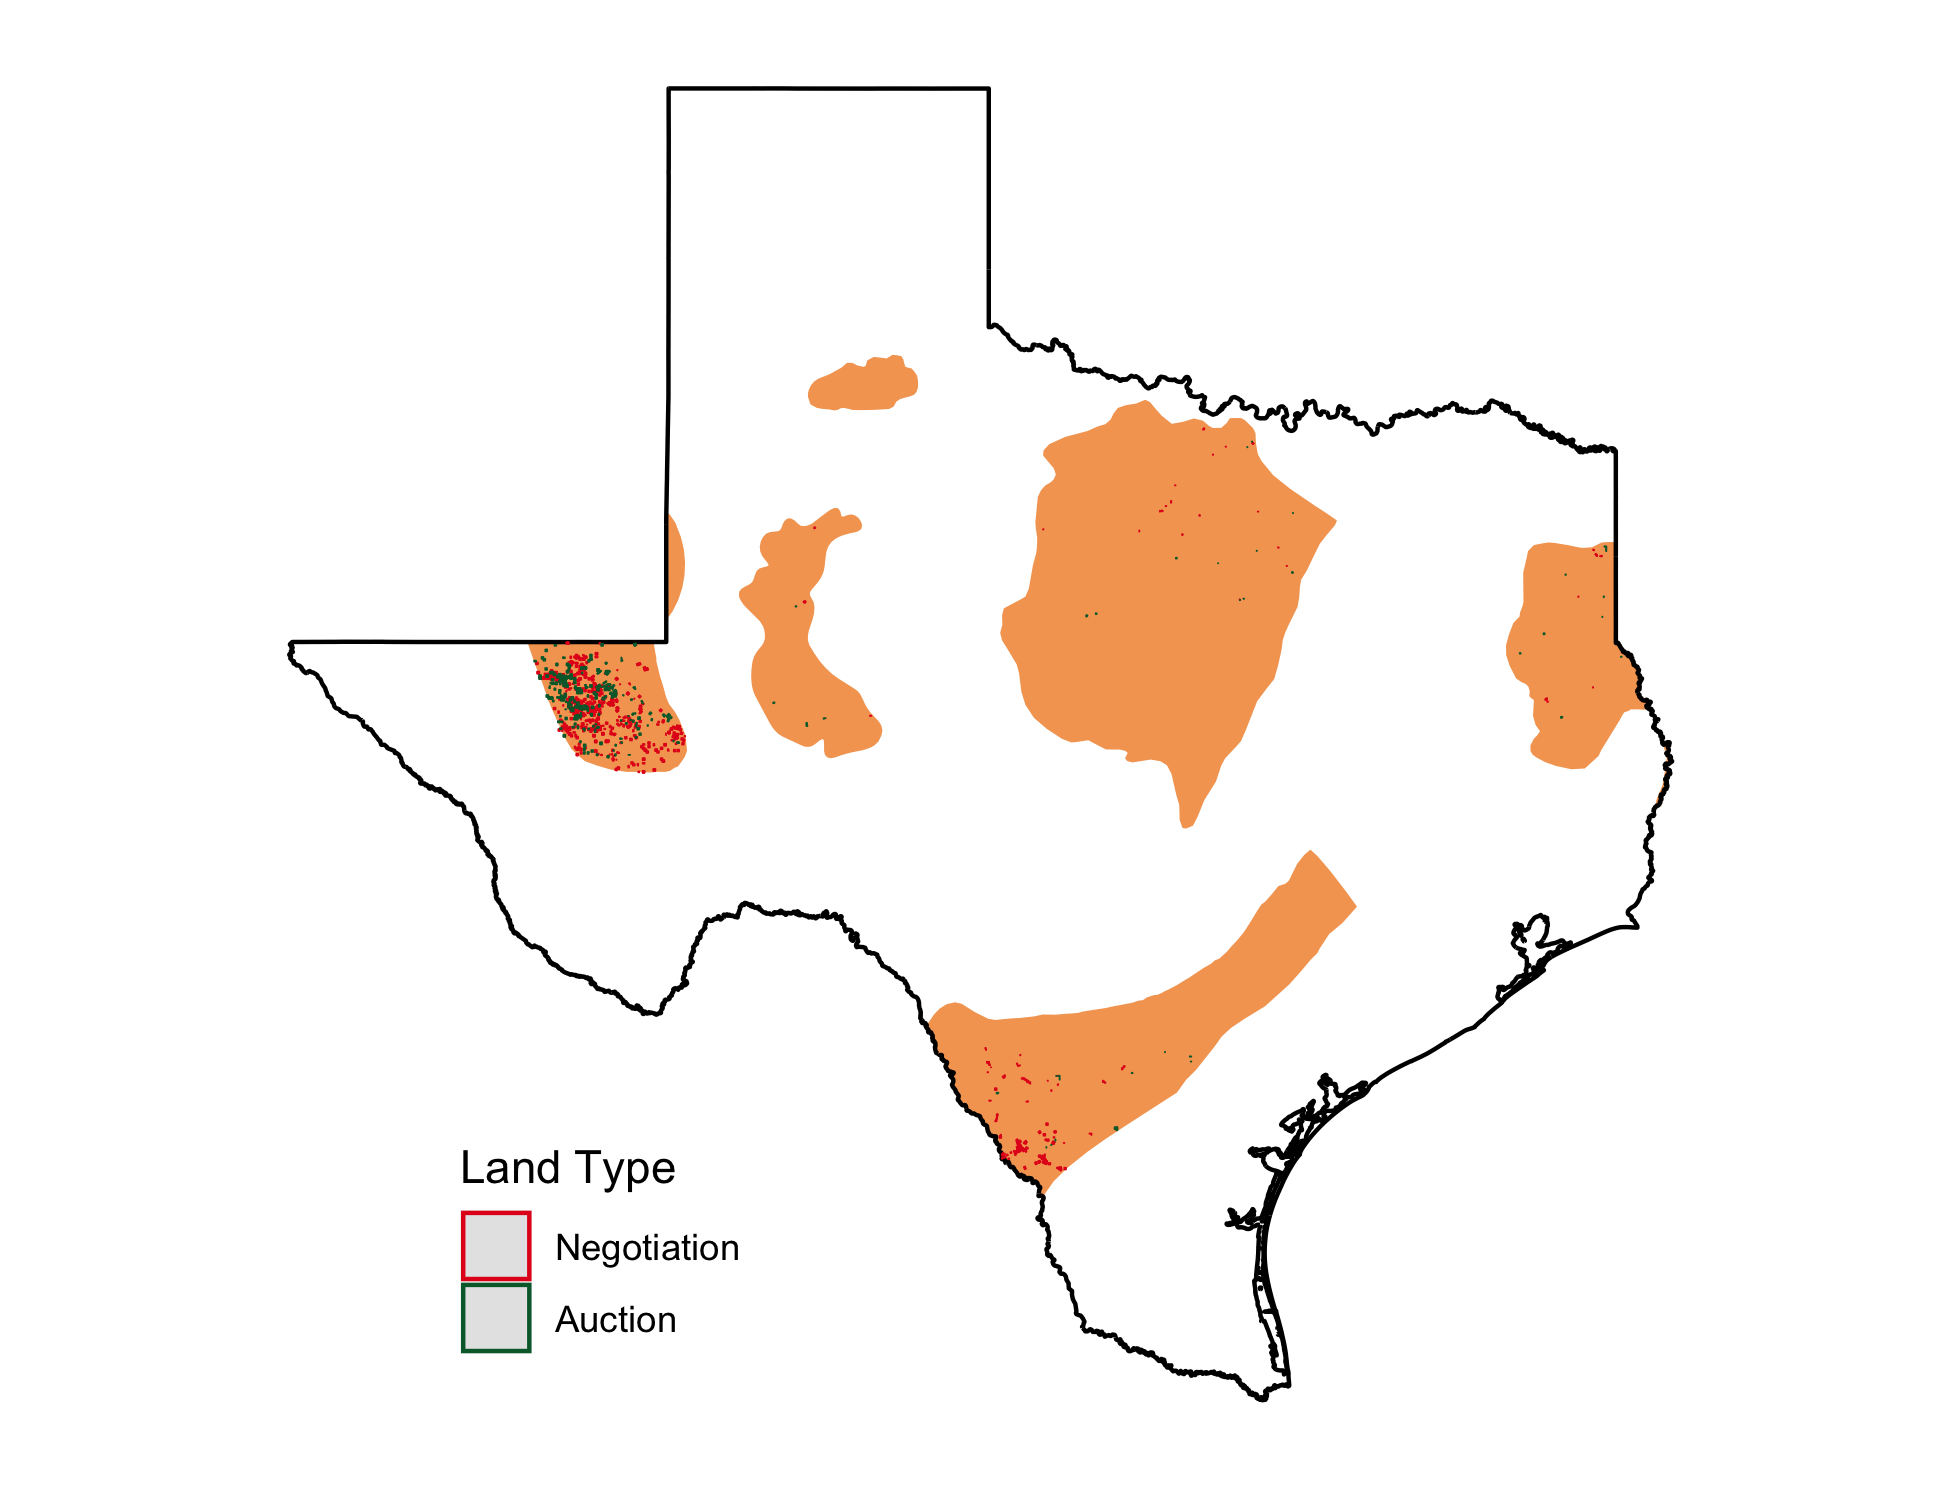
\includegraphics[width=1\textwidth]{../output/figures/glo_leases_in_texas.png}
\par\end{centering}
\end{figure}

\subsection{Additional Lease Results}\label{sec:extra_regressions}

%\addtolength{\tabcolsep}{6pt}
\begin{table}[H]
	\begin{center}
	\begin{threeparttable}
		\caption{Bonus Payments and Mechanism Type, per Acre}
		\label{tab:table_main_bonus_levels}
		\small
		
\begin{tabular}{lccccccccc}
\toprule
 & ( 1 ) & ( 2 ) & ( 3 ) & ( 4 ) & ( 5 ) & ( 6 ) & ( 7 ) & ( 8 ) & ( 9 )\\
\midrule
 & 0.63 & 0.66 & 0.82 & 0.64 & 0.78 & 0.66 & 0.77 & 0.87 & 1.06\\

\multirow{-2}{*}{\raggedright\arraybackslash Auction} & (0.14) & (0.18) & (0.28) & (0.19) & (0.11) & (0.19) & (0.10) & (0.34) & (0.19)\\

\midrule
Grid & 10 & 10 & 10 & 20 & DML & 10 & DML & 10 & DML\\

Time & Q & GY,Q & GYQ & GY,Q & DML & GY,Q & DML & GY,Q & DML\\

Extra & No & No & No & No & No & Yes & Yes & No & No\\

Private Only & No & No & No & No & No & No & No & Yes & Yes\\

N & 1,515 & 1,515 & 1,515 & 1,515 & 1,515 & 1,260 & 1,260 & 1,308 & 1,308\\

$R^2$ & 0.728 & 0.880 & 0.901 & 0.807 &  & 0.868 &  & 0.890 & \\
\bottomrule
\end{tabular}
            
		\begin{tablenotes}
		\footnotesize
		\item The dependent variable in each regression is the the lease's bonus payment per acre. In columns 1-4, the size of the location bins, in miles, are indicated in the ``Grid'' row, while the structure of the time controls (``Q'' for quarter of sample, ``GY,Q'' for grid-by-year plus quarter of sample, and ``GYQ'' for grid-by-quarter of sample) are indicated in the ``Time'' row.  Standard errors are clustered by grid in columns 1-4.  Column 5 uses a double/debiased machine learning routine, as recommended in \cite{chernozhukov2018double}.  Fixed effect models include a spline in lease size while the DML model includes lease size as a random forest covariates.  
		\end{tablenotes}
	\end{threeparttable}
	\end{center}
\end{table}



\addtolength{\tabcolsep}{-4pt}
\begin{table}[H]
	\begin{center}
	\begin{threeparttable}
	\caption{Lease Bonus Regressions with Controls for Royalty Rate and Term}
	\label{tab:BonusWithRoyaltyTerm}
	\small
	
\begin{tabular}{lcccccc}
\toprule
 & ( 1 ) & ( 2 ) & ( 3 ) & ( 4 ) & ( 5 ) & ( 6 )\\
\midrule
 & 0.72 & 0.68 & 0.96 & 0.43 & 0.43 & 0.57\\

\multirow{-2}{*}{\raggedright\arraybackslash Auction} & (0.18) & (0.16) & (0.13) & (0.06) & (0.05) & (0.05)\\

\midrule
Estimate & G10Y & G20Y & DML & G10Y & G20Y & DML\\

Outcome & Bonus per acre & Bonus per acre & Bonus per acre & log(Bonus) & log(Bonus) & log(Bonus)\\
\midrule

N & 1,515 & 1,515 & 1,515 & 1,515 & 1,515 & 1,515\\
\bottomrule
\end{tabular}
            
		\begin{tablenotes}
		\footnotesize
		\item The dependent variable is either bonus per acre (in thousands per acre) or the natural logarithm of the bonus payment.  The Grid10-Year and Grid20-Year fixed-effect specifications include a spline in lease acreage and linear terms for term length and royalty rate, while the DML specifications include these variables as  random forest covariates.     
		\end{tablenotes}	   
	\end{threeparttable}
	\end{center}
\end{table}

\begin{table}[H]
	\begin{center}
	\begin{threeparttable}
	\caption{Lease Output Regressions with Controls for Royalty Rate and Term}
	\label{tab:OutputWithRoyaltyTerm}
	\small
	
\begin{tabular}{lcccccc}
\toprule
  & ( 1 ) & ( 2 ) & ( 3 ) & ( 4 ) & ( 5 ) & ( 6 )\\
\midrule
 & 3.85 & 4.44 & 6.14 & 0.53 & 0.77 & 0.75\\

\multirow{-2}{*}{\raggedright\arraybackslash Auction - Lease Revenue} & (1.46) & (1.54) & (1.90) & (0.20) & (0.22) & (0.08)\\

N & 1,259 & 1,259 & 1,259 & 746 & 980 & \vphantom{1} 1,259\\

\midrule
 & 1.17 & 1.32 & 1.55 & 0.62 & 0.83 & 0.81\\

\multirow{-2}{*}{\raggedright\arraybackslash Auction - Output} & (0.41) & (0.41) & (0.43) & (0.21) & (0.25) & (0.24)\\

N & 1,259 & 1,259 & 1,259 & 746 & 980 & 1,259\\

\midrule
 & 1.31 & 1.56 & 2.16 & 0.48 & 0.65 & 0.84\\

\multirow{-2}{*}{\raggedright\arraybackslash Auction - Seller Revenue} & (0.39) & (0.39) & (0.49) & (0.12) & (0.14) & (0.23)\\

N & 1,259 & 1,259 & 1,259 & 1,259 & 1,259 & 1,259\\

\midrule
Estimate & G10Y & G20Y & DML & G10Y & G20Y & DML\\

Estimator & Linear & Linear & Linear & Poisson & Poisson & Poisson\\
\bottomrule
\end{tabular}
            
		\begin{tablenotes}
		\footnotesize
		\item The dependent variables are per-acre (lease and seller revenue in thousands per acre, output in hundreds of BOE per acre) in the linear specifications and in aggregate (not per acre) in the Poisson specifications.  The Grid10-Year and Grid20-Year fixed-effect specifications include a spline in lease acreage and linear terms for term length and royalty rate, while the DML specifications include these variables as  random forest covariates.    
		\end{tablenotes}	   
	\end{threeparttable}
	\end{center}
\end{table}

\addtolength{\tabcolsep}{10pt}
\begin{table}[H]
	\begin{center}
	\begin{threeparttable}
		\caption{Drilled Regressions}\label{tab:drilledregs}
		 \small
			 
\begin{tabular}{lccccc}
\toprule
 & ( 1 ) & ( 2 ) & ( 3 ) & ( 4 ) & ( 5 )\\
\midrule
 & 0.07 & 0.05 & 0.08 & 0.07 & 0.04\\

\multirow{-2}{*}{\raggedright\arraybackslash Auction} & (0.03) & (0.04) & (0.06) & (0.03) & (0.03)\\

\midrule
Grid & 10 & 10 & 10 & 20 & DML\\

Time & Q & GY,Q & GYQ & GY,Q & DML\\

N & 1,259 & 1,259 & 1,259 & 1,259 & 1,259\\

$R^2$ & 0.375 & 0.626 & 0.719 & 0.489 & \\
\bottomrule
\end{tabular}
            
			\footnotesize
			\begin{tablenotes}
				\item The dependent variable is equal to 1 if a lease was drilled during its primary term and 0 otherwise.  The sample includes all leases whose primary term ends before March, 2019.  In columns 1-4, the size of the location bins, in miles, are indicated in the ``Grid'' row, while the structure of the time controls (``Q'' for quarter of sample, ``GY,Q'' for grid-by-year plus quarter of sample, and ``GYQ'' for grid-by-quarter of sample) are indicated in the ``Time'' row.  Standard errors are clustered by grid in columns 1-4.  Column 5 uses a double/debiased machine learning routine.  Fixed effect models include a spline in lease size and the DML model includes lease size as a random forest covariate.
			\end{tablenotes} 
	\end{threeparttable}
	\end{center}
\end{table}
	
	\begin{table}[H]
	\begin{center}
	\begin{threeparttable}
		\caption{Log Output Regressions Among the Sample of Leases That Are Drilled}\label{tab:outputconddrilled}
		 \small
			 
\begin{tabular}{lccccc}
\toprule
 & ( 1 ) & ( 2 ) & ( 3 ) & ( 4 ) & ( 5 )\\
\midrule
 & 0.40 & 0.52 & 0.33 & 0.58 & 0.45\\

\multirow{-2}{*}{\raggedright\arraybackslash Auction} & (0.19) & (0.20) & (0.25) & (0.22) & (0.17)\\

\midrule
Grid & 10 & 10 & 10 & 20 & DML\\

Time & Q & GY,Q & GYQ & GY,Q & DML\\

N & 425 & 425 & 425 & 425 & 425\\

$R^2$ & 0.652 & 0.856 & 0.909 & 0.774 & \\
\bottomrule
\end{tabular}
            
			\footnotesize
			\begin{tablenotes}
				\item The dependent variable is the natural logarithm of discounted barrels of oil equivalent (Output) per acre.  The sample includes all drilled leases whose primary term ends before March, 2019.  In columns 1-4, the size of the location bins, in miles, are indicated in the ``Grid'' row, while the structure of the time controls (``Q'' for quarter of sample, ``GY,Q'' for grid-by-year plus quarter of sample, and ``GYQ'' for grid-by-quarter of sample) are indicated in the ``Time'' row.  Standard errors are clustered by grid in columns 1-4.  Column 5 uses a double/debiased machine learning routine.  Fixed effect models include a spline in lease size and the DML model includes lease size as a random forest covariate.
			\end{tablenotes} 
	\end{threeparttable}
	\end{center}
\end{table}
\addtolength{\tabcolsep}{-10pt}

\subsection{Unleased Spell Duration Analysis}\label{app:duration}
Our lease and parcel data make it possible to reliably identify which parcels have active leases starting in January, 2001.  We leases to their parcels using our existing parcel-lease map and then merge this with our lease revenue data, which starts in January, 2001.  We define a lease as active during a given month if that month is during the lease's primary term or if that month is spanned by the earliest and latest royalty payments we observe for the lease.  We say a lease is terminated at the later of a lease's primary term expiration and its last observed royalty payment.  If a given terminated lease is the only lease currently active in a parcel, we say that parcel is \textit{unleased} at that point.  As soon as another lease is signed that is associated with a parcel, we say the parcel as \textit{leased} again.  With this structure, every parcel in our data is either leased or unleased on January 1, 2001, and for every subsequent month, and we use this parcel-by-month panel to construct ``unleased spells'' for every parcel.  It is worth noting that parcels which are unleased as of January 1, 2001 may have been unleased previous to this point.  As a result, unleased spells that begin in January, 2001 may be left-censored.  

In the unleased spell analyses that follow, we define four samples of unleased spells.  The ``All'' spell sample is everything described above, while the ``First'' spell sample is just the first unleased spell for each parcel.  The ``Uncensored'' spell sample excludes unleased spells that begin in January, 2001, because we do not know whether they began earlier than January 2001 or not.  Finally, the ``First Uncensored'' spell sample is the first uncensored unleased spell for each parcel.  Table \ref{tab:SpellDefs} tabulates how many spells we have under each of these definitions, for RAL and State parcels, starting in each year between 2001 and 2019.

\begin{table}[htbp]
	\begin{center}
		\begin{threeparttable}
			\caption{Parcel Unleased Spell Counts}\label{tab:SpellDefs}
			\label{tab:summary_stats}
			\small
			
\begin{tabular}{rrrrrrrrr}
\toprule
\multicolumn{1}{c}{ } & \multicolumn{2}{c}{All} & \multicolumn{2}{c}{Uncensored} & \multicolumn{2}{c}{First} & \multicolumn{2}{c}{First Uncensored} \\
\cmidrule(l{3pt}r{3pt}){2-3} \cmidrule(l{3pt}r{3pt}){4-5} \cmidrule(l{3pt}r{3pt}){6-7} \cmidrule(l{3pt}r{3pt}){8-9}
Year & RAL & State & RAL & State & RAL & State & RAL & State\\
\midrule
2001 & 1439 & 450 & 17 & 10 & 1439 & 450 & 17 & 10\\
2002 & 20 & 1 & 20 & 1 & 20 & 1 & 20 & 1\\
2003 & 234 & 61 & 234 & 61 & 233 & 61 & 233 & 61\\
2004 & 72 & 4 & 72 & 4 & 59 & 4 & 72 & 4\\
2005 & 22 & 5 & 22 & 5 & 10 & 5 & 19 & 5\\
2006 & 24 & 10 & 24 & 10 & 2 & 1 & 21 & 10\\
2007 & 36 & 2 & 36 & 2 & 1 & 1 & 31 & 2\\
2008 & 57 & 1 & 57 & 1 & 4 & 0 & 44 & 1\\
2009 & 162 & 23 & 162 & 23 & 8 & 2 & 67 & 15\\
2010 & 163 & 89 & 163 & 89 & 2 & 2 & 138 & 58\\
2011 & 62 & 25 & 62 & 25 & 1 & 0 & 43 & 23\\
2012 & 46 & 10 & 46 & 10 & 4 & 0 & 30 & 7\\
2013 & 78 & 10 & 78 & 10 & 1 & 0 & 47 & 10\\
2014 & 37 & 2 & 37 & 2 & 0 & 0 & 19 & 1\\
2015 & 44 & 17 & 44 & 17 & 1 & 2 & 16 & 8\\
2016 & 106 & 58 & 106 & 58 & 2 & 4 & 16 & 24\\
2017 & 97 & 8 & 97 & 8 & 1 & 2 & 33 & 7\\
2018 & 77 & 10 & 77 & 10 & 1 & 0 & 31 & 5\\
2019 & 18 & 13 & 18 & 13 & 3 & 0 & 6 & 0\\
\bottomrule
\end{tabular}

			\footnotesize
			\begin{tablenotes}
				\item ``All'' refers to all unleased spells on on-shale PSF parcels since January 1, 2001.  ``Uncensored'' spells are the subset of those parcels which were already leased on January 1, 2001.  The date at which these spells begin is thus uncensored.  ``First'' spells are the subset of all spells which are the first unleased spell for a given parcel, and ``First Uncensored'' spells are the subset of uncensored spells which are the first unleased, uncensored spell for a given parcel.
			\end{tablenotes}
		\end{threeparttable}
	\end{center}
\end{table}

Our first test of the hypothesis that RAL and State parcels experience differentially long unleased spells makes use of the adjusted Kaplan-Meier survival curve estimator, derived in \cite{xie2005adjusted}.  This estimate of  survival curves is similar to traditional ``unadjusted'' non-parametric survival curve estimate in experimental data, with the main difference being that each observation is weighted by the inverse of a propensity score.  Here we estimate the probability that a spell on a parcel in a given location, of a given size, at a given point in time, is on an RAL or State parcel using a fixed-effects logit model, with Grid-by-year and Year-by-quarter fixed effects, as well as a spline in parcel acres.  Letting $\widehat{p}_i$ be the estimated propensity score for spell $i$, we assign a weight of $\frac{1}{\widehat{p}_i}$ to spells on State parcels, and a weight of $\frac{1}{1-\widehat{p}_i}$ to RAL parcels.  As described above, we estimate these survival curves under four different samples of unleased spells, as shown in figures \ref{fig:km10} and \ref{fig:km20}.\footnote{We use the \texttt{ipw.survival} command from the R language package \texttt{RISCA}.}  Under both 10-mile and 20-mile grid fixed effects, as well as all four sample definitions, there is no visual difference in ``survival'' between the two samples.  Unleased spells on State and RAL parcels seem to end equally quickly.

\begin{figure}[H]
	\centering
	\caption{Covariate-Adjusted Kaplan-Meier Survival Curves: Grid 10 Specifications}\label{fig:km10}
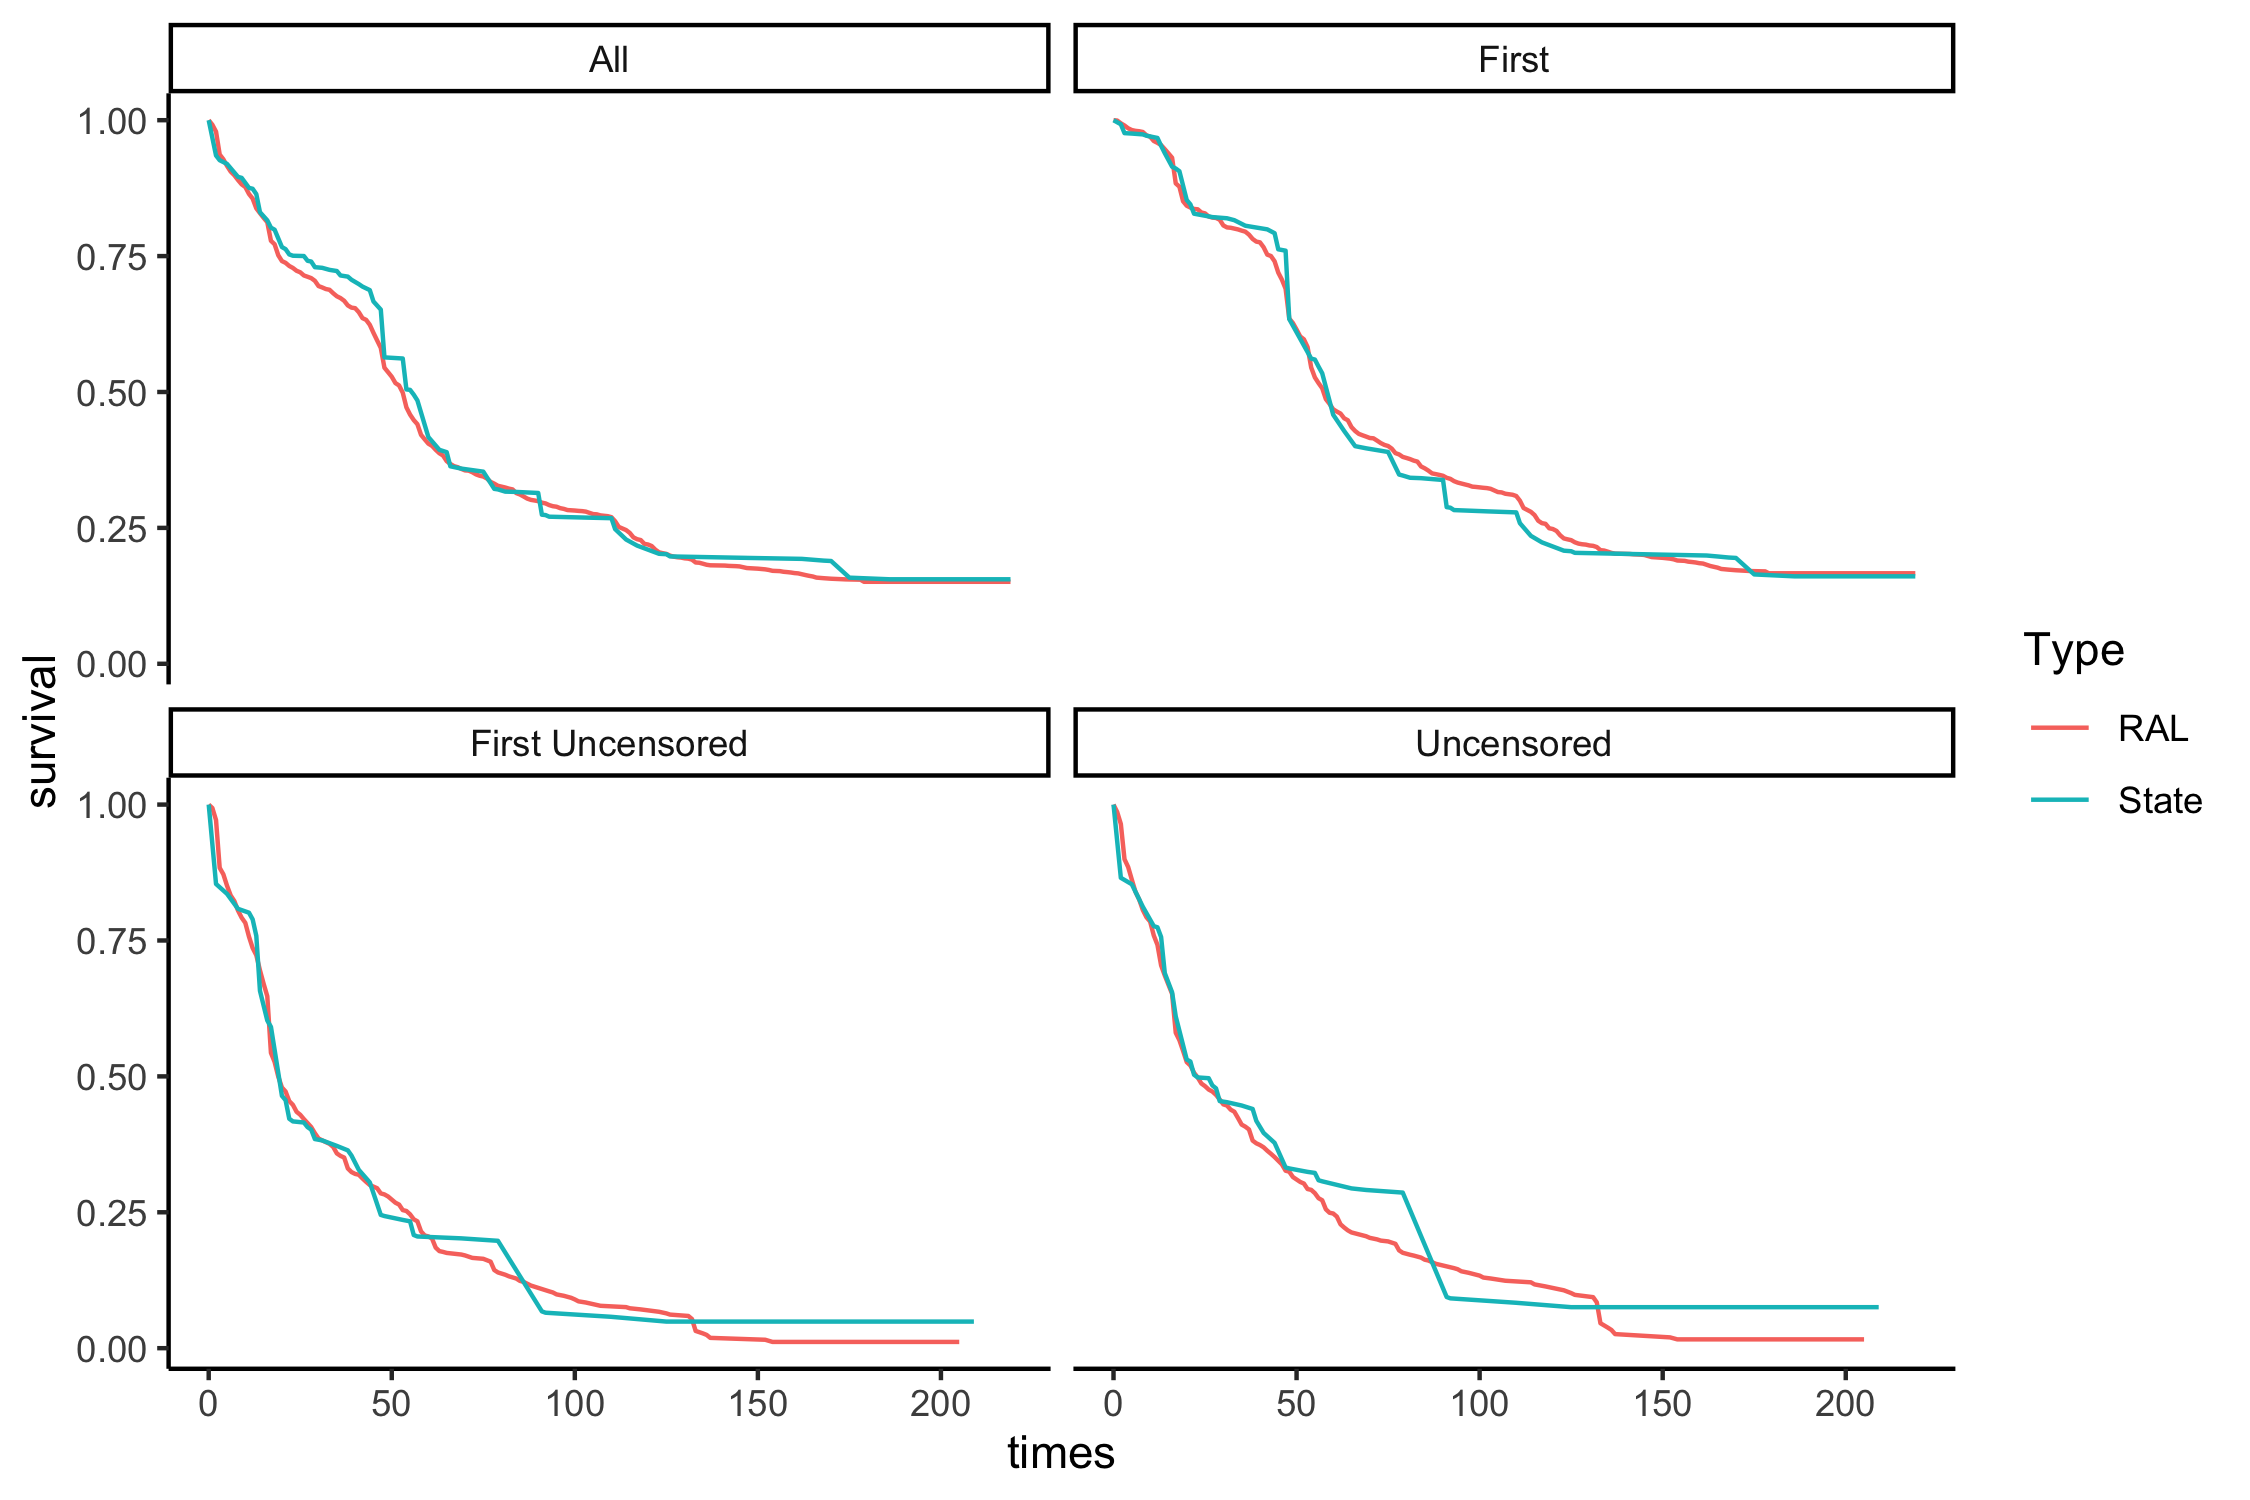
\includegraphics[width=1\textwidth]{../output/figures/ipwkm10.png}
\end{figure}

\begin{figure}[H]
	\centering
	\caption{Covariate-Adjusted Kaplan-Meier Survival Curves: Grid 20 Specifications}\label{fig:km20}
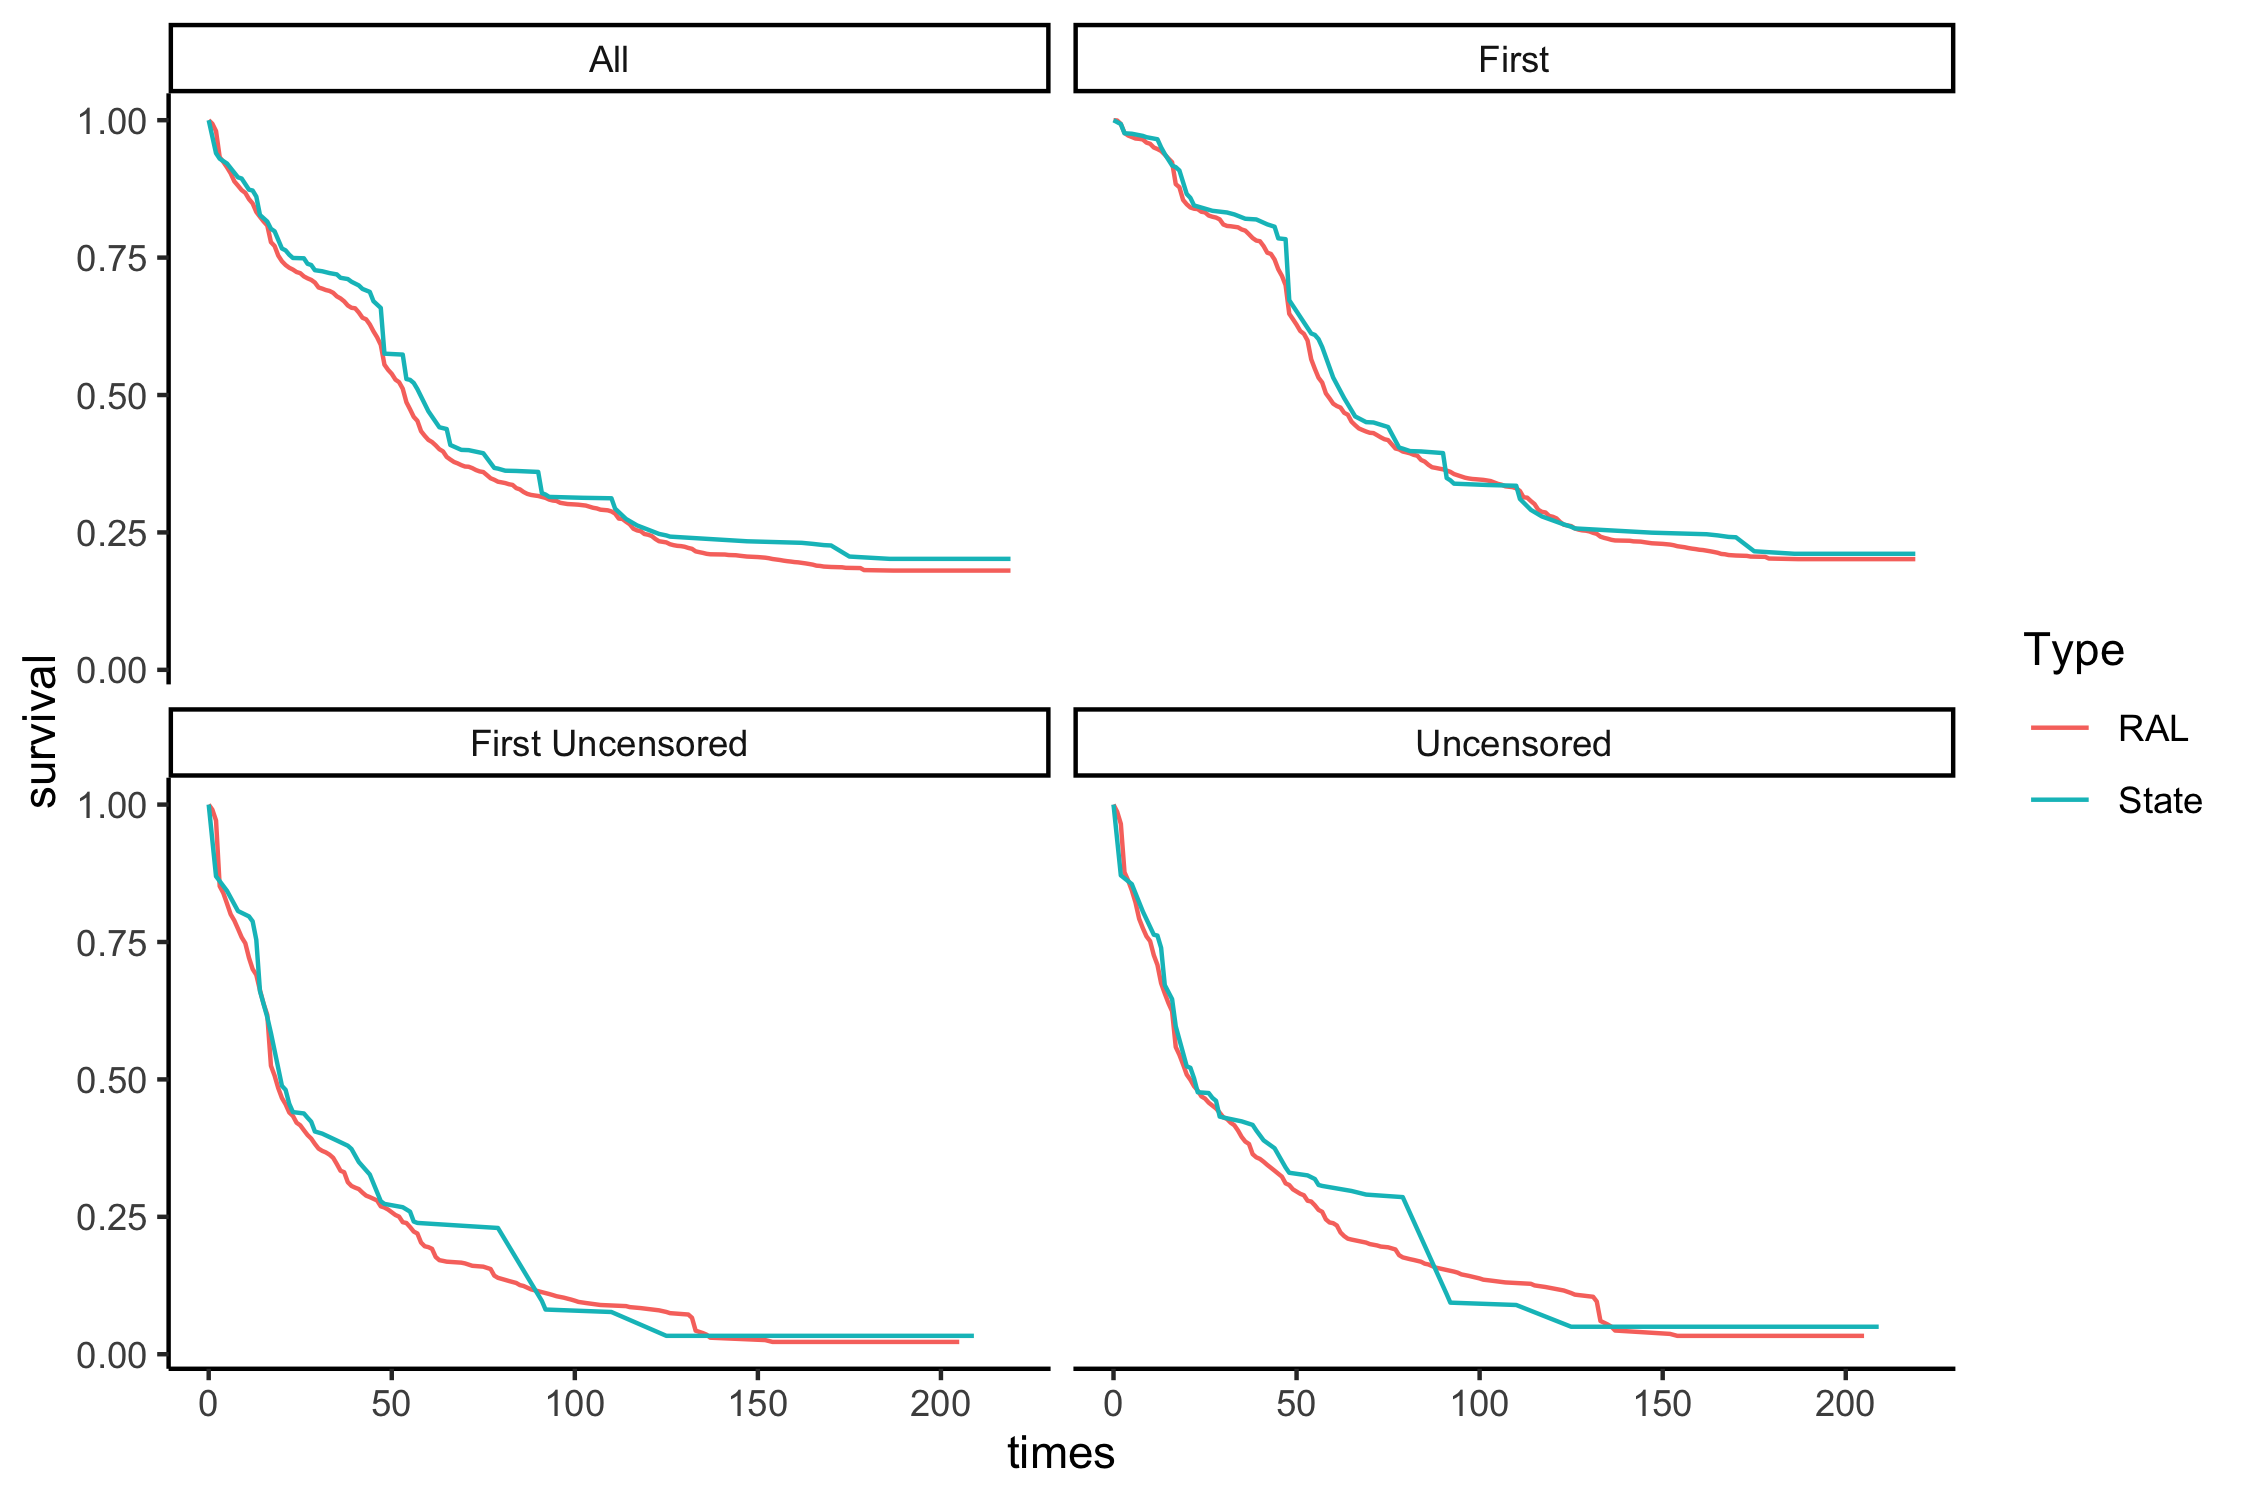
\includegraphics[width=1\textwidth]{../output/figures/ipwkm20.png}
\end{figure}

To formalize the test we have so far conducted visually, we compute adjusted log-rank tests of the hypothesis that two samples have the same hazard function, again informed by the ideas in \cite{xie2005adjusted}.  As in the adjusted survival curve estimates, the adjusted log-rank test weighs each observation by a propensity score.  \cite{xie2005adjusted} shows that as long as the propensity scores are consistently estimated, the adjusted log-rank test is distributed as standard normal, allowing us to use traditional asymptotic inference techniques.  Because we estimate our propensity scores using fixed effects in a high dimension non-linear model, we also compute p-values for these tests using the randomization inference technique recommended in \cite{xie2005adjusted}, as well as a standard non-parametric bootstrap.  Table \ref{tab:logrank} reports the test statistic values and p-values for the null hypothesis that the two survival curves are identical under each of these sample definitions, grid sizes, and inferential techniques.  There is no specification in which we can reject the null hypothesis under conventional significance thresholds that State and RAL unleased spells have the same survival function.  

\begin{table}[htbp]
	\begin{center}
		\begin{threeparttable}
			\caption{Log-Rank Tests of the Hypothesis That RAL and State Parcels Have Equally Long Unleased Spells}\label{tab:logrank}
			\small
			
\begin{tabular}{l>{\raggedleft\arraybackslash}p{8em}>{\raggedleft\arraybackslash}p{8em}>{\raggedleft\arraybackslash}p{8em}>{\raggedleft\arraybackslash}p{8em}}
\toprule
  & All & Uncensored & First & First Uncensored\\
\midrule
\addlinespace[0.3em]
\multicolumn{5}{l}{\textbf{Grid 10}}\\
\hspace{1em}statistic & -0.82 & -0.72 & -0.16 & -0.54\\
\hspace{1em}p.value & 0.41 & 0.47 & 0.87 & 0.59\\
\hspace{1em}ripval & 0.36 & 0.50 & 0.86 & 0.57\\
\hspace{1em}bspval & 0.42 & 0.47 & 0.88 & 0.60\\
\hspace{1em}N & 2,892 & 1,408 & 1,788 & 900\\
\addlinespace[0.3em]
\multicolumn{5}{l}{\textbf{Grid 20}}\\
\hspace{1em}statistic & 1.561 & 0.874 & 1.118 & 1.234\\
\hspace{1em}p.value & 0.119 & 0.382 & 0.263 & 0.217\\
\hspace{1em}ripval & 0.096 & 0.384 & 0.242 & 0.215\\
\hspace{1em}bspval & 0.152 & 0.389 & 0.263 & 0.213\\
\hspace{1em}N & 3,297. & 1,579. & 2,086. & 1,030.\\
\bottomrule
\end{tabular}

			\footnotesize
			\begin{tablenotes}
				\item ``Statistic'' is the log-rank statistic for the hypothesis that RAL and State parcels have equally long unleased spells.  Under the null hypothesis, this statistic is normally distributed with mean 0, and variance 1.  The first p-value compares this statistic to the quantiles of the standard normal distribution.  The second p-value (``ripval'') comes from a randomization inference procedure: randomly assign treatment according to the propensity scores, recompute the test statistic, and repeat 1000 times.  This p-value compres the original statistic to the distribution of the simulated statistics.  Finally, the third p-value, ``bspval'', comes from non-parametrically bootstrapping the entire testing process 1000 times and comparing the original statistic to its standardized bootstrap distribution.
				\item ``All'' refers to all unleased spells on on-shale PSF parcels since January 1, 2001.  ``Uncensored'' spells are the subset of those parcels which were already leased on January 1, 2001.  The date at which these spells begin is thus uncensored.  ``First'' spells are the subset of all spells which are the first unleased spell for a given parcel, and ``First Uncensored'' spells are the subset of uncensored spells which are the first unleased, uncensored spell for a given parcel.  Sample sizes differ in the top and bottom panels because the propensity score procedure will drop spells that lie in grids and/or time periods with either all RAL or all State leases, and grids of different sizes will result in a different number of dropped observations.
			\end{tablenotes}
		\end{threeparttable}
	\end{center}
\end{table}
	
\addtolength{\tabcolsep}{-6pt}

\subsection{RAL Lessor Heterogeneity}\label{app:lessor_hetero}
To document the extent to which different kinds of RAL lessors experience different leasing outcomes, we use lessor names to specify two notions of lessor sophistication.  First, we simply count how many leases a lessor has signed in recent history, going back to the year 2000.  Among all lessors who have signed an RAL lease overlying a shale formation since 2000, only 31\% signed more than one lease, 5\% signed five or more, and only 1\% signed 10 or more.  However, those highly experienced lessors signed many of the leases in our sample: 28\% of RAL leases are signed by lessors who have signed 5 or more since 2000, and 13\% are signed by lessors who have signed 10 or more.  It seems reasonable to expect that more experienced lessors employ more sophisticated negotiation tactics.  Second, we infer a lessor's sophistication from its name.  Lessors who are firms\footnote{We flag a lessor as a firm if its name contains one or more of the following strings: ``inc'', ``ltd'', ``llc', ``lp'', ``corp'', ``asset'', ``assoc'', ``company'', ``holdings'', ``partner'', or ``manag''.} and perhaps especially lessors that are firms explicitly working in the oil and gas business\footnote{We flag a lessor as working in the oil and gas business if its name contains one or more of the following strings: ``oil'', ``gas'', ``production'', ``explor'', ``mineral''.} may also employ more sophisticated negotiation tactics, so we generate flags for these two characteristics.  

We include dummy variables for each of these categories in our standard log bonus regressions, shown in Table \ref{tab:LessorHet}.  Across specifications, more experienced and/or more sophisticated lessors do seem to negotiate moderately higher bonus payments, but the differences are often imprecise, especially in the specifications that have 10-mile grid fixed effects. Moreover, while these lessors do better than novice negotiators, they still perform substantially worse than auctions. For example, consider specification 6, which uses 20-mile grid fixed effects and includes a dummy for lessors with 10 or more leases.  These lessors negotiate bonuses that are 10 log points higher than other RAL lessors, but since the average RAL lease has a bonus that is 54 log points lower than auctioned leases, this is still 44 log points lower than than the State's auction.

\addtolength{\tabcolsep}{5pt}
\begin{table}[H]
\begin{center}
\begin{threeparttable}
	\caption{RAL Lessor Heterogeneity and Bonus Payments}
	\label{tab:LessorHet}
 	\small
   	
\begin{tabular}{lcccccccc}
\toprule
 & ( 1 ) & ( 2 ) & ( 3 ) & ( 4 ) & ( 5 ) & ( 6 ) & ( 7 ) & ( 8 )\\
\midrule
 & 0.54 & 0.54 & 0.54 & 0.53 & 0.54 & 0.54 & 0.54 & 0.53\\

\multirow{-2}{*}{\raggedright\arraybackslash Auction} & (0.06) & (0.06) & (0.06) & (0.06) & (0.07) & (0.07) & (0.07) & (0.07)\\

 & 0.03 & \phantom{X} & \phantom{X} & \phantom{X} & 0.07 & \phantom{X} & \phantom{X} & \phantom{X}\\

\multirow{-2}{*}{\raggedright\arraybackslash LessorExperience5} & (0.04) & \phantom{X} & \phantom{X} & \phantom{X} & (0.03) & \phantom{X} & \phantom{X} & \phantom{X}\\

 & \phantom{X} & 0.07 & \phantom{X} & \phantom{X} & \phantom{X} & 0.10 & \phantom{X} & \phantom{X}\\

\multirow{-2}{*}{\raggedright\arraybackslash LessorExperience10} & \phantom{X} & (0.07) & \phantom{X} & \phantom{X} & \phantom{X} & (0.05) & \phantom{X} & \phantom{X}\\

 & \phantom{X} & \phantom{X} & 0.04 & \phantom{X} & \phantom{X} & \phantom{X} & 0.11 & \phantom{X}\\

\multirow{-2}{*}{\raggedright\arraybackslash LessorIsFirm} & \phantom{X} & \phantom{X} & (0.04) & \phantom{X} & \phantom{X} & \phantom{X} & (0.03) & \phantom{X}\\

 & \phantom{X} & \phantom{X} & \phantom{X} & 0.00 & \phantom{X} & \phantom{X} & \phantom{X} & 0.13\\

\multirow{-2}{*}{\raggedright\arraybackslash LessorIsEP} & \phantom{X} & \phantom{X} & \phantom{X} & (0.07) & \phantom{X} & \phantom{X} & \phantom{X} & (0.08)\\

\midrule
Grid & 10 & 10 & 10 & 10 & 20 & 20 & 20 & 20\\

Time & GY,Q & GY,Q & GY,Q & GY,Q & GY,Q & GY,Q & GY,Q & GY,Q\\

N & 1,515 & 1,515 & 1,515 & 1,515 & 1,515 & 1,515 & 1,515 & 1,515\\

$R^2$ & 0.961 & 0.961 & 0.961 & 0.961 & 0.945 & 0.945 & 0.945 & 0.945\\
\bottomrule
\end{tabular}
            
    \footnotesize
    \begin{tablenotes}
    	\item Regressions of the log of the bonus payment onto an auction indicator, as well as indicators for various measures of lessor sophistication.  LessorExperience5 refers to lessors who lease at least 5 times during 2000-2016, and LessorExperience10 requires 10 or more leases.  LessorIsFirm refers to lessors whose names suggest they are corporations, not natural people.  LessorIsEP refers to lessors whose names suggest they are experienced in the oil and gas industry.  All specifications include a spline in lease acres. 
    \end{tablenotes}
\end{threeparttable}
\end{center}
\end{table}

We also measure the extent to which the gap between auctioned and negotiated bonuses depends on the size of the lease. Our motivation for this analysis is that many of the actions involved with negotiating improved lease terms involve fixed costs which are invariant to the size of the lease. If the underlying value of a lease was exactly proportional to its size, then we might expect the owners of bigger leases to take more action to improve lease terms than the owners of smaller lessors do. Table \ref{tab:LeaseSizeHet} revisits the log bonus regressions from Table \ref{tab:table_main_bonus}. In column 1, we eschew our acres controls, project log bonus \textit{per acre} onto just a dummy for auction and grid-time fixed effects. Next we include an additional dummy for whether a negotiated lease is larger than the sample median size. Columns 2 and 5 show that under this constant returns to scale assumption (ie no spline in acres), big negotiated leases do pay a modest amount more than small negotiated leases. However, there are a variety of reasons to suspect that the underlying value of a lease is not proportional to size, since modern shale drilling requires large blocks of contiguous acreage to drill long horizontal wells and to efficiently co-locate surface equipment for many neighboring wells. Columns 3 and 6 re-introduce a spline in acres, as in the main specifications in the text. The results now show that negotiated leases above the median perform no better than those below the median, relative to the bonuses achieved at auction for each size group. 

\addtolength{\tabcolsep}{5pt}
\begin{table}[H]
\begin{center}
\begin{threeparttable}
	\caption{Lease Size Heterogeneity and Bonus Payments}
	\label{tab:LeaseSizeHet}
 	\small
   	
\begin{tabular}{lcccccc}
\toprule
 & ( 1 ) & ( 2 ) & ( 3 ) & ( 4 ) & ( 5 ) & ( 6 )\\
\midrule
 & 0.53 & 0.57 & 0.52 & 0.52 & 0.55 & 0.50\\

\multirow{-2}{*}{\raggedright\arraybackslash Auction} & (0.06) & (0.07) & (0.06) & (0.07) & (0.09) & (0.08)\\

 & \phantom{X} & 0.07 & -0.02 & \phantom{X} & 0.06 & -0.04\\

\multirow{-2}{*}{\raggedright\arraybackslash BigNegotiation} & \phantom{X} & (0.03) & (0.04) & \phantom{X} & (0.04) & (0.04)\\

\midrule
CRS & Yes & Yes & No & Yes & Yes & No\\

Estimate & G10Y & G10Y & G10Y & G20Y & G20Y & G20Y\\
\midrule

N & 1,515 & 1,515 & 1,515 & 1,515 & 1,515 & 1,515\\
\bottomrule
\end{tabular}
            
    \footnotesize
    \begin{tablenotes}
    	\item The variable ``BigNegotiation'' is equal to 1 if the lease is negotiated and if it is larger than the median negotiated lease, approximately \inputy{../output/estimates/negotiation_med_size.tex} acres; otherwise it is 0.  The dependent variable in the CRS specifications is the natural logarithm of bonus \textit{per acre}, while it is the natural logarithm of the bonus in the non-CRS specifications.  The non-CRS specifications in columns 3 and 6 include a spline in lease acres. All regressions include Grid10-Year or Grid20-Year fixed effects, and all include Year-Quarter fixed effects.
    \end{tablenotes}
\end{threeparttable}
\end{center}
\end{table}

This analysis provides a test of the hypothesis that the negotiations in this paper perform particularly badly because of the fact that RAL lessors only receive half of the proceeds they negotiate. In this sample, the average lease above the median is nearly five times larger than the average lease below the median. This implies that the differential incentive for effort across the two groups is much larger than the differential between RAL lessors and fully private lessors. Nevertheless, even in the CRS case, the maximum amount of the auction-negotiation gap that could be explained by shirking is small. Once we flexibly control for lease size, we find no evidence that large negotiated leases perform better than smaller negotiated leases. 

\pagebreak

\subsection{Lease-Parcel Comparison}\label{app:lease-parcel-decomp}
In this appendix, we present comparisons of lease level and parcel level regressions run on samples which are more immediately comparable than those presented in the main text. Table \ref{tab:lease_parcel_linear} presents linear results and \ref{tab:lease_parcel_Poisson} presents Poisson results. 

Columns 1-3 present lease level regressions, using 10 mile or 20 mile grid fixed effects, or DML spatial controls. Compared to the lease regressions presented in Section \ref{sec:ResultsLease}, we make two changes. First, we use the entire population of leases signed between 2004 and 2013. As described in Section \ref{sec:sampleSelection}, the main lease sample excludes RAL leases with features that do not overlap with auction leases, such as being too big or too small, or having multiple ownership interests. However, these lease level features are not defined at the parcel level. We thus include all leases when computing parcel level outcomes. Second, we discount all outcomes to 2004 (as opposed to the date the lease was signed). All models in Section \ref{sec:ResultsLease} include quarter of sample fixed effects, to account for large changes in fracking technology and oil prices over time. However, the parcel regressions are inherently cross-sectional. To facilitate comparison with the parcel regressions, we eschew all time controls here. 

Columns 4-6 present the corresponding parcel-level regressions. Compared to the results presented in Table \ref{tab:ParcelOutcomes}, there is only one change. Here we restrict the sample to parcels which sign at least one lease between 2004 and 2013, since these are the parcels underlying the lease sample in the first part of the table. 

Comparing across corresponding lease and parcel results reveals differences which are much smaller than the comparison discussed in Section \ref{sec:ParcelOutcomes}. In levels, the bonus results are slightly higher at the parcel level, while the output results are slightly lower. In logs, the bonus results are comparable, while the lease output and revenue results are twice as large. These small differences stem from two remaining factors which are fundamentally different across the two regressions: parcel vs. lease weighting and acreage controls. All models include a spline in acres. However leases may be much smaller or much bigger than their underlying parcel(s). When they are larger, a single transaction will receive more weight in the parcel regression than other transactions on single parcels. Conversely, re-leases of a parcel after expiration will receive \textit{less} weight in the parcel regression than in the lease regression, as will multiple concurrent smaller leases on a parcel. 

\addtolength{\tabcolsep}{-6pt}

\begin{table}[H]
\begin{center}
\begin{threeparttable}
	\caption{Lease Parcel Comparison: Linear Models}
	\label{tab:lease_parcel_linear}
 	\small
   	
\begin{tabular}{lcccccc}
\toprule
  & ( 1 ) & ( 2 ) & ( 3 ) & ( 4 ) & ( 5 ) & ( 6 )\\
\midrule
 & 0.354 & 0.394 & 0.352 & 0.515 & 0.558 & 0.491\\

\multirow{-2}{*}{\raggedright\arraybackslash Auction - Bonus} & (0.073) & (0.107) & (0.063) & (0.116) & (0.155) & (0.067)\\

\midrule
 & 0.425 & 0.457 & 0.469 & 0.243 & 0.384 & 0.299\\

\multirow{-2}{*}{\raggedright\arraybackslash Auction - Output} & (0.159) & (0.166) & (0.186) & (0.278) & (0.257) & (0.182)\\

\midrule
 & 1.699 & 1.784 & 1.916 & 0.794 & 1.329 & 1.396\\

\multirow{-2}{*}{\raggedright\arraybackslash Auction - Lease Revenue} & (0.597) & (0.683) & (0.712) & (1.084) & (1.048) & (0.677)\\

\midrule
 & 0.832 & 0.909 & 0.877 & 0.772 & 0.960 & 0.849\\

\multirow{-2}{*}{\raggedright\arraybackslash Auction - Seller Revenue} & (0.178) & (0.232) & (0.199) & (0.321) & (0.339) & (0.183)\\

\midrule
Estimate & G10 & G20 & DML & G10 & G20 & DML\\

Sample & All Leases & All Leases & All Leases & Leased Parcels & Leased Parcels & Leased Parcels\\

N & 2,389 & 2,389 & 2,389 & 1,784 & 1,784 & 1,784\\
\bottomrule
\end{tabular}
            
    \footnotesize
    \begin{tablenotes}
    	\item Outcomes are per acre and all models include a cubic spline in acres with 1 knot at the median lease or parcel size.  
    \end{tablenotes}
\end{threeparttable}
\end{center}
\end{table}

\begin{table}[H]
\begin{center}
\begin{threeparttable}
	\caption{Lease Parcel Comparison: Poisson Models}
	\label{tab:lease_parcel_Poisson}
 	\small
   	
\begin{tabular}{lcccccc}
\toprule
  & ( 1 ) & ( 2 ) & ( 3 ) & ( 4 ) & ( 5 ) & ( 6 )\\
\midrule
 & 0.716 & 0.777 & 0.717 & 0.690 & 0.729 & 0.644\\

\multirow{-2}{*}{\raggedright\arraybackslash Auction - Bonus} & (0.109) & (0.128) & (0.075) & (0.088) & (0.110) & (0.053)\\

\midrule
 & 0.520 & 0.691 & 0.425 & 0.218 & 0.350 & 0.198\\

\multirow{-2}{*}{\raggedright\arraybackslash Auction - Output} & (0.152) & (0.153) & (0.171) & (0.154) & (0.112) & (0.114)\\

\midrule
 & 0.509 & 0.653 & 0.430 & 0.189 & 0.332 & 0.200\\

\multirow{-2}{*}{\raggedright\arraybackslash Auction - Lease Revenue} & (0.148) & (0.168) & (0.166) & (0.140) & (0.129) & (0.112)\\

\midrule
 & 0.608 & 0.696 & 0.526 & 0.370 & 0.470 & 0.350\\

\multirow{-2}{*}{\raggedright\arraybackslash Auction - Seller Revenue} & (0.101) & (0.116) & (0.105) & (0.087) & (0.090) & (0.063)\\

\midrule
Estimate & G10 & G20 & DML & G10 & G20 & DML\\

Sample & All Leases & All Leases & All Leases & Leased Parcels & Leased Parcels & Leased Parcels\\

N & 2,389 & 2,389 & 2,389 & 1,784 & 1,784 & 1,784\\
\bottomrule
\end{tabular}
            
    \footnotesize
    \begin{tablenotes}
    	\item Outcomes are in levels and all models include a cubic spline in acres with 1 knot at the median lease or parcel size.  
    \end{tablenotes}
\end{threeparttable}
\end{center}
\end{table}

\section{Data Cleaning \label{sec:DataCleaning}}

\subsection{Sample construction \label{sec:AppendixSampleConstruction}}

Table \ref{tab:waterfall} presents the number of negotiated and auctioned leases existing in original data provided to us by GLO, as well as the subset that survives each of our sample restrictions. We begin with the universe of GLO leases signed between 2004 and 2016 that can be matched to original PSF parcels and have non-missing lease characteristics.  We first drop leases on PSF land types other than Relinquishment Act land or belonging entirely to the GLO.  Next, we use the EIA's definition of shale formations in Texas, shown shaded in yellow in Figure \ref{fig:RAL_map}, to drop leases on land that does not overlie a shale formation.  To ensure a comparable distribution of lease covariates, we drop especially small leases, especially large leases, and leases with especially short primary terms.  We drop leases on ``undivided'' mineral interests, which occur when two or more parties share ownership of the surface and or mineral estate.\footnote{For example, if parents John and Mary bequeath their 640 acre parcel to their two children, Bob and Jane, then Bob and Jane each have an undivided interest in the parcel.  In principal, it is possible for Bob and Jane to separately lease their respective undivided interests to different oil and gas companies.} We drop a small number of leases on non-RAL land that are allocated via bilateral negotiation specifically because only one party can economically use the land.   Similarly, we drop RAL leases that are allocated by auction when the State is unable to determine who the rightful surface owner is.  Finally, we drop non-standard negotiated agreements between the State of Texas and E\&P companies that do not have the traditional mineral lease contract structure.

\begin{table}[H]
	\begin{center}
	\begin{threeparttable}
		\caption{Sample Construction}
		\label{tab:waterfall}
		\small
		
\begin{tabular}{llrr}
\toprule
 & Drop Reason & Negotiation & Auction\\
\midrule
Initial Sample &  & 4,828 & 827\\
 & Not RAL or State lease & 4,368 & 786\\
 & Not on Shale & 2,517 & 553\\
 & Less Than 10 or Greater Than 1,000 Acres & 1,985 & 499\\
 & Gross and Net Acreage Differ & 1,658 & 497\\
 & Undivided Interest & 1,092 & 493\\
 & Term Less Than 1 Year & 1,073 & 493\\
 & Negotiated State Lease & 1,066 & 493\\
 & Auctioned RAL Lease & 1,066 & 454\\
 & Nonstandard Lease Category & 1,061 & 454\\
Final Sample &  & 1,061 & 454\\
\bottomrule
\end{tabular}
            
		\footnotesize
		\begin{tablenotes}
			\item Additional discussion provided in Section \ref{sec:sampleSelection}.
		\end{tablenotes}
	\end{threeparttable}
	\end{center}
\end{table}

\subsection{Firm Names \label{sec:FirmNameCleaning}}
Though we observe the name of the firm on the lease, E\&P companies sometimes use intermediaries, or ``landmen,'' to acquire land, and, in these cases, we might not observe the relevant firm. One reason why a firm would do this would be to prevent its competitors from discovering its interest in a particular play before it had had acquired enough land to develop it. This ``secrecy'' motivation is probably relevant, because the presence of non-E\&P company lessees is much more common in the auction data than in the negotiated data. This is perhaps not surprising, since the auction records are publicly released shortly after the auction, and easily observable.  To partially overcome this challenge, we use data on \textit{lease assignments}, legal transactions which formally change ownership of a lease from one firm to another, to better infer who the ultimate E\&P company is on leases initially awarded to non-E\&P company lessees. We observe assignments on 18\% of RAL leases and 33\% of auction leases. For each non-E\&P company in our data who ever assigns a lease to an E\&P company, we identify a variety of ``most common'' assignees, using auction status, location and time.  For non-E\&P company leases in which we do not observe an assignment, we characterize the ``real'' lessee as this (conditional) most common assignee.  Though this process is not perfect, it does greatly reduce the number of leases that we believe are allocated to lessees that are not E\&P companies.

\pagebreak

\section{Double/Debiased Machine Learning Estimation Details}\label{sec:dml}

To non-parametrically control for the effects of location and time on lease terms and lease outcomes, we adopt the double/debiased machine learning framework of \cite{chernozhukov2018double}, which we refer to as ``DML'' models.  In our partially linear DML models, we use the partially linear model derived in equation 4.4 of that paper.  In our pseudo-Poisson models, we derive a Neyman-orthogonal score for pseudo-Poisson regression, documented below.  

In all DML models, we implement the nuisance parameter estimation with random forests, using the \texttt{regression\_forest} function from the \texttt{grf} package for the R language, as described in \cite{athey2019generalized}, with 1000 trees per forest.  Following the suggestions in \cite{chernozhukov2018double}, we construct a single point estimate and covariance matrix of the relevant parametric terms using 5-fold cross-fitting, and report the ``median'' values of these across 101 randomized cross-fitted partitions, as in definition 3.3 of that paper. 

To derive the Neyman-orthogonal moment for pseudo-Poisson regression, we closely follow the discussion following Lemma 2.5 of \cite{chernozhukov2018double}.  Let $Y$ be a non-negative outcome, $D$ a \textit{binary} covariate, and $X$ a vector of controls that we wish to model non-parametrically, like location, time and lease or parcel size.  Our goal is to pick the values of $\theta$ and $\beta(X)$ that minimize a pseudo-Poisson quasi-log-likelihood criteria:
\begin{equation*}
	(\theta_0, \beta(X)_0) = \arg \max_{\theta, \beta(X)} \mathbb{E}\left[Y(D\theta + \beta(X))-\exp(D\theta + \beta(X))\right]
\end{equation*}

Let $\beta_{\theta}(x)$ be the best fitting value of $\beta(x)$ for a given value of $\theta$.  For the above criterion, we can find this implicitly by setting the gradient of the \textit{conditional} expectation of the criterion with respect to $\beta(x)$ equal to 0, and re-arranging terms:
\begin{equation*}
	\exp(\beta_{\theta}(x)) = \frac{\gamma(x)}{\exp(\theta)\delta(x) + 1 - \delta(x)}
\end{equation*}	
where $\gamma(x) = \mathbb{E}\left[Y\mid X = x\right]$ and $\delta(x) = \mathbb{E}\left[D\mid X = x\right]$.  The Neyman-orthogonal moment for pseudo-Poisson regression is the total derivative of the quasi-log-likelihood criterion with respect to $\theta$, after we plug in the solution for $\exp(\beta_{\theta}(x))$:
\begin{equation*}
	\psi(Y, D, X; \theta, \gamma(x), \delta(x)) = \left(Y-\frac{\exp(D\theta)\gamma(X)}{\exp(\theta)\delta(X) + 1 - \delta(X)}\right)\left(D - \frac{\exp(\theta)\delta(X)}{\exp(\theta)\delta(X) + 1 - \delta(X)}\right).
\end{equation*}
This is the objective whose empirical average we set to 0 in our pseudo-Poisson regressions.

\section{Empirical Auction Analysis Details}\label{sec:AppendixAuction}

We estimate the distribution of bidder values, conditional on observable and unobservable auction-level heterogeneity, in the independent private values framework\footnote{Though \textit{offshore} mineral leasing has long been studied in the common values framework (e.g., \cite{hendricks_empirical_1988}, most recent analysis of \textit{onshore} mineral lease auctions takes place in the private values framework.  \cite{kong2016sequential} and \cite{kong_selective_2017} both provide informative discussions about why private values make sense in studying the recent shale boom.}, by following the model in \cite{roberts2013unobserved}.  The first step is to regress the natural logarithm of an auction's reserve price $R$, in nominal dollars per acre, on a cubic spline in its size in acres $f(A)$, and fixed effects for the tract's county $\delta_{c}$ and the date the auction took place $\gamma_{t}$.
\begin{equation*}
	\log R_i = f(A_i) + \delta_{c(i)} + \gamma_{t(i)} + \epsilon_i
\end{equation*}
We define the observed heterogeneity index as the predicted value from this regression, $H_i = \widehat{f}(A_i) + \widehat{\delta}_{c(i)} + \widehat{\gamma}_{t(i)}$, and the unobserved heterogeneity index as $U_i = \log R_i - H_i$, the residual.  We estimate this model on the entire population of GLO auctions for tracts in counties that overlap shale formations, during 2004-2016, including auctions that do not receive any bids at or above the reserve price.

Next, we use $(H_i,U_i)$ as the heterogeneity covariates in the procedure specified in section 4 of \cite{guerre2000optimal}.  After recovering the bidder values that are consistent with equilibrium bidding, we find that the bid-value relationship is occasionally non-monotonic.  When this occurs, we follow the advice in \cite{chernozhukov2009improving} and re-order estimated values within an auction to guarantee monotonicity.

Table \ref{tab:AuctionNBidsRobust} shows how our key auction statistics are sensitive to different kernel bandwidth choices, dropping bids near the boundary of the support of the distribution of bids and/or heterogeneity covariates, and dropping auctions where value re-arrangement is necessarily to maintain monotonicity of the bid-value relationship.
\addtolength{\tabcolsep}{4pt}
\begin{table}[H]
\begin{center}
\begin{threeparttable}
	\caption{Auction Robustness}
	\label{tab:AuctionNBidsRobust}
 	\small
   	
\begin{tabular}{lcc>{\centering\arraybackslash}p{7em}>{\centering\arraybackslash}p{7em}}
\toprule
Sample & Bandwidth Scaling & Auctions & Average 1-to-2 Markup & Average 1-to-2 Allocative Gain\\
\midrule
All & 0.5 & 202 & 0.34 & 0.41\\
All & 1.0 & 202 & 0.34 & 0.47\\
All & 2.0 & 202 & 0.34 & 0.58\\
Drop Trimmed & 1.0 & 154 & 0.32 & 0.40\\
Drop Rearranged & 1.0 & 162 & 0.36 & 0.49\\
Drop Trimmed and Rearranged & 1.0 & 117 & 0.34 & 0.41\\
\bottomrule
\end{tabular}
            
    \footnotesize
    \begin{tablenotes}
    	\item This table summarizes bids from GLO auctions with 2 or more bidders across various assumptions made in the GPV analysis.  The sample includes all auctions in the first three rows.  In the fourth row we drop auctions where one or more bids would be trimmed under the GPV trimming rules.  In the fifth row we drop auctions where the estimated pseudovalues are not monotonic in the bids.  In the sixth row, we drop auctions where bids would be either trimmed or pseudovalues would need to be rearranged to impose monotonicity. ``Bandwidth Scaling'' refers to whether we use the Silverman rule for bandwidth selection (1.0) or half (0.5) or twice (2.0) the Silverman rule. The ``1-to-2 Markup'' is the natural logarithm of the ratio of the winning bid to the second highest bid.  The ``1-to-2 Allocative Gain'' is the natural logarithm of the ratio of the GPV pseudovalues of the winning and second highest bids.
    \end{tablenotes}
\end{threeparttable}
\end{center}
\end{table}

\pagebreak

\section{RAL Lease Addenda}\label{sec:Appendix_Addenda}
In addition to specifying bonus payments, royalty rates and primary terms, mineral leases also specify how the contracting parties will resolve disagreements about issues related to environmental impact, on-site water usage, and surface property disruptions, among other things.  These protective clauses are standardized in the GLO auction lease agreement, and there are ``default'' values for them in the GLO's required RAL lease agreement.  However, RAL surface owners and their contracting partners can optionally negotiate some deviations from the standard lease.  To the extent that RAL surface owners are willing to forego up-front bonus payments for stricter surface protections during subsequent exploration and production, we might be worried that the differences in bonus payments that we observe are not caused by the mechanism itself, but rather by a compensating differentials story.  

It is important to note that it is not possible to directly condition on the content of these protective clauses and maintain our causal interpretation of the differences between auctioned and negotiated leases, for the same reason that we do not condition on royalty rates and primary terms.  See the discussion at the end of Section \ref{sec:ResultsLease}.  However, having recognized the challenge in interpreting these results as causal, we explore the extent to which RAL lease addenda content affects our regression estimates.

To do this, we had a team of research assistants do a dual-entry review of the text of these lease addenda for all RAL leases signed between 2005 and 2016.  They characterized the extent to which each one improved or deteriorated the surface owner's rights along dimensions such as environmental impact, water usage, and surface property disruptions, guided by the procedure in \cite{vissing_one--many_2017}.  About 73\% of RAL leases have one or more additional clauses in their lease addenda.  In Table \ref{tab:table_bonus_addenda}, we include measures of these protective clauses in bonus and output regressions like those shown in Table \ref{tab:table_main_bonus} and \ref{tab:output_stacked}.  The first two columns mirror the result shown in the main text: auctioned pleases pay 50 or more log points in up-front bonus payments than negotiated leases do, and output is similarly higher.  In the next two columns, we include covariates which measure the number of pages in an RAL lease's addendum, as well as the number of specific legal clauses documented.  Finally, in the last two columns we include covariates for each specific kind of clause that occur in these addenda, coded as $-1$ if a lease's addenda deteriorates the surface owner's rights, relative to the standard RAL lease, $0$ if it is absent or does not affect the surface owner's rights, and $+1$ if it improves upon the surface owner's rights.  Across all specifications, we find no evidence that variation between auctioned and negotiated leases in protective clauses can ``explain away'' the observed differences in both bonus payments and output. 

\begin{table}[H]
\begin{center}
\begin{threeparttable}
	\caption{Bonus Payments, Lease Output, and Mechanism Type: Robustness to RAL Lease Addenda}
	\label{tab:table_bonus_addenda}
 	\small
   	
\begin{tabular}{lcccccc}
\toprule
  & ( 1 ) & ( 2 ) & ( 3 ) & ( 4 ) & ( 5 ) & ( 6 )\\
\midrule
 & 0.57 & 0.65 & 0.61 & 0.80 & 0.61 & 0.70\\

\multirow{-2}{*}{\raggedright\arraybackslash Auction - log(Bonus)} & (0.06) & (0.05) & (0.06) & (0.07) & (0.06) & (0.06)\\

N & 1,409 & 1,409 & 1,409 & 1,409 & 1,409 & 1,409\\

\midrule
 & 1.10 & 1.39 & 1.23 & 1.66 & 1.16 & 1.32\\

\multirow{-2}{*}{\raggedright\arraybackslash Auction - Output} & (0.34) & (0.44) & (0.42) & (0.52) & (0.43) & (0.44)\\

N & 1,153 & 1,153 & 1,153 & 1,153 & 1,153 & 1,153\\

\midrule
Addenda Controls & None & None & Pages + Clauses & Pages + Clauses & Individual & Individual\\

Grid & 10 & DML & 10 & DML & 10 & DML\\

Time & GY,Q & DML & GY,Q & DML & GY,Q & DML\\
\bottomrule
\end{tabular}
            
    \footnotesize
    \begin{tablenotes}
    	\item Columns 1 and 2 report baseline specifications with no controls RAL lease addenda content.  We measure lease addenda content in columns 3 and 4 using the number of pages and number of individual clauses in the addenda.  In Columns 5 and 6, we include a set of individual dummy variables indicating whether the addenda improves (+1), deteriorates (-1) or is similar to the standard auction lease (0) along each of these margins: Surface Protection, Payment Terms, Location Requirements, Pugh Clause, Cleanup Terms, Livestock Protection, On-site Water Use, Waste Management, Definitional Changes, Pollution Protection, Infrastructure Constraints, Caliche Use, Additional Fees, Time Constraints, Miscellaneous. Columns 1, 3, and 5 control for space and time using 10-mile grid by year of sample fixed effects, as well as fixed effects for quarter of sample.  Columns 2, 4, and 6 use a double/debiased machine learning routine, as recommended in \cite{chernozhukov2018double}, with non-parametric controls for lease latitude, longitude, effective date, size and addenda measures.  Sample includes leases signed between 2005-2016.
    \end{tablenotes}
\end{threeparttable}
\end{center}
\end{table}

\end{appendices}

\end{document}



